\documentclass[12pt,letterpaper]{book}
\usepackage{amsmath}
\usepackage{amssymb}
\usepackage{amsthm}
\usepackage[colorlinks=true]{hyperref}
\usepackage{graphicx}
\usepackage{cancel}
\usepackage{xcolor}
\usepackage[english]{babel}
\usepackage{bm}
\usepackage{simplewick}
\usepackage[toc,page]{appendix}
%\usepackage{bbold}
\setlength{\textwidth}{180mm}
\setlength{\oddsidemargin}{-1cm}
\setlength{\evensidemargin}{-1cm}
%\setlength{\topmargin}{-40pt}
\def\lt{<} % compatibility with instiki
\def\gt{>} % compatibility with instiki
\newtheoremstyle{example}{\topsep}{\topsep}%
     {}%         Body font
     {}%         Indent amount (empty = no indent, \parindent = para indent)
     {\bfseries}% Thm head font
     {}%        Punctuation after thm head
     {\newline}%     Space after thm head (\newline = linebreak)
     {\thmname{#1}\thmnumber{ #2}\thmnote{ #3}}%         Thm head spec

   \theoremstyle{example}
   \newtheorem{example}{Example}[subsection]
%%comment the aproppiate line
\newcommand{\tofc}[1]{#1} % if full
%\renewcommand{\tofc}[1]{} %if  \includeonly{chapter1}
%\includeonly{introduction}
\begin{document}
\tofc{
\renewcommand{\thepage}{\roman{page}}
\tableofcontents{}

\newpage{}
}

\renewcommand{\thepage}{\arabic{page}}
\setcounter{page}{1}

%$x^2$
%instiki:category: QuantumFieldTheory
%instiki:
%instiki:***
%instiki:
%instiki:[[Beyond|Contents]]
%instiki:
%instiki:***

\chapter*{Introduction}
\label{cha:introduction} %noinstiki

\addcontentsline{toc}{chapter}{Introduction} %noinstiki

We have organized the topics in order of complexity, and, in the same
spirit than in  previous book \cite{lsm}, we have tried to write the
calculations as detailed as possible. In
Chapter 
\ref{cha:second-quantization} %noinstiki [[Chapter II]]
we included the building blocks
of quantum field theory, in Chapter 
\ref{cha:s-matrix} %noinstiki [[Chapter III]]
we introduce
the $S$--matrix in the Scr\"odinger Picture separating the kinematical
and normalization factors from the matrix element. Then the expressions
for the decay rates and cross sections are obtained. The explicit
calculation of the matrix element from the expansion of the
$S$--matrix to obtain the Feynman rules, is postponed to Chapter
\ref{chap:fr}. %noinstiki [[Chapter V]].
In Chapter 
\ref{cha:two-body-decays} %noinstiki [[Chapter IV]]
we use the Feynman
rules necessary to calculates the matrix element, and develop the
techniques associated to the squaring of the matrix element. In
Chapter 
\ref{chap:fr} %noinstiki [[Chapter V]]
we obtain the Feynman rules used in two body
decays directly from the first order expansion of the $S$--matrix in
the interaction picture. The subsequent chapters have applications of
the techniques developed to the calculation of tree-level, 
Chapter 
\ref{cha:three-body-decays} %noinstiki [[Chapter V]]
and loop processes.


This notes are based in books \cite{Maggiore:2005qv}, \cite{Mandl:1985bg}, \cite{Lahiri:2005sm}.  In each Chapter or Section the main reference used is cited. Also, we have included material developed by students Juan Alberto Yepez, Jos\'e David Ruiz \'Alvarez. This notes are written in English, because at this level it is expected that any physics student be fluently in reading technical texts in this language.

Some parts are still in Spanish. 

This work have been partially supported by ``Dedicaci\'on Exclusiva 2008-2009''  project: RR 26663

%%% Local Variables: 
%%% mode: latex
%%% TeX-master: "beyond"
%%% End:
%instiki:category: QuantumFieldTheory
\chapter{Second quantization}
\label{cha:second-quantization} %noinstiki
%instiki:
%instiki:***
%instiki:
%instiki:[[Beyond|Contents]]
%instiki:
%instiki:***
%instiki:
%instiki:* [Fock space for real scalar fields](#fock-space-real)
%instiki:
%instiki:* [Quantization of Fermions](#quant-ferm)
%instiki:


Two key ingredients to formulate the Quantum Field Theory (QFT) are the quantization of systems in which the particles can be created and destroyed (quamtum theory of radiation) and the behavior of relativistic systems. When both ingredients are present the particles can be understood as the excited modes of certain field. When the particles in a system are not relativistic, the formalism of creation and annihilation operators is just an alternative method to describe the Hamiltonian of the Schr\"odinger equation. In relativistic systems however, the existence of negative energy states force the construction of new quantum states, the Fock states, in order to have proper defined probabilities for the states of the system. In section xx we start by building the Fock states associated to a massless not relativistic scalar field. Then we generalize the results to a massive scalar field satisfying the Klein-Gordon equation.

Some parts of the discussion were based in some topics of chapters 4-6 of \cite{Maggiore:2005qv}.


In general, the formalism of second quantization is usefull to describe the states of an undetermined number of particles and interactions which do not conserve particle number. In addition to high-energy physics where any number of particles may be created or annihilated during a collision process, in statistitical physics it becomes useful to describe a macroscopic body using the grand-canonical statistical ensemble, in which the number of particles is allowed to fluctuate. In condensed-matter states the interactions may modify also the number of various excitation quanta, such as phonons. A more general formalism to discuss this systems is developed in Appendix~\ref{cha:green-functions}.

\section{Quantization of the nonrelativistic string}
\label{sec:fock-space-real}

\subsection{The clasical string}
\label{sec:clasical-string}
\begin{frame}[fragile,allowframebreaks]
In conventional quantization the energy of one state is interpreted as the possible eigenstates of an Hamiltonian operator acting on the states of the system. 
\begin{align}
  \widehat{H}|\text{State}\rangle=E|\text{State}\rangle
\end{align}
One step further is to consider the wave function as the eigenstate  of the operator--field acting on certain \emph{Fock states}
\begin{align}
\label{eq:1}
  \widehat{\Phi}|\text{Fock State}\rangle=\Phi||\text{Fock State}\rangle\,,
\end{align}
Like that usual quantum mechanical observable, the wave function will have an uncertainty. 
The Fock states are the states under which the classical wave function can be obtained with a small uncertainty
\begin{align}
    \Phi\pm\Delta\Phi=\langle\text{Fock State}|\widehat{\Phi}|\text{Fock State}\rangle
\end{align}
This happens when the number of quanta of the Fock state is big enough. In fact, a state with a definite number of quanta has a infinity uncertainty \cite{Gross:1993}.

Eq.~\eqref{eq:1} is the basis for the calculation of cross section and decay widths in quantum field theory. Now we will study how to define a such Fock state for a scalar field.


We have already see in Chapter 1 of \cite{lsm} that a string have a collective wave motion that is described by a continuous field, which satisfies the familiar one-dimensional wave equation
\begin{align}
\label{eq:2}
  \frac{1}{v^2}\frac{\partial^2\phi}{\partial t^2}-\frac{\partial^2\phi}{\partial z^2}=0
\end{align}
This equation can be derived following two different paths. The first is to decomposing the string into individual oscillators for which the usual Lagrangian formalism can be used. The second is just by formulating certain Lagrangian density from which the equation of motion can be obtained  by using the Euler-Lagrange equation
\begin{align}
  \partial_\mu\left[\frac{\partial\mathcal{L}}{\partial(\partial_\mu\phi)}\right]-\frac{\partial\mathcal{L}}{\partial\phi}=0\,.
\end{align}
In the first approach the string is considered to be composed of $N$ oscillators coupled together  by springs with a spring constant $k$. At certain time $t$, the displacement of the oscillator $i$ at time $t$ is represented by $\phi_i(t)$. In Table~\ref{tab:1} it is displayed the corresponding macroscopic quantities. Note also that $1/v^2=\mu/T$.
\begin{table}[htp!]
  \centering
  \begin{tabular}{l|l}
    micro & macro \\\hline{}
    $l$ & $L=N l$\\
    $m$ & $\mu=m/l$ \\
    $k$ & $T=k l$\\
    $\phi_i(t)=\phi(z_i,t)$ &  $\phi(z,t)$\\
  \end{tabular}
  \caption{From micro to macro}
\label{tab:1}
\end{table}
It is worth to stress that at the Lagrangian level, which is the sum of each individual oscillator Lagrangian, it is the sum of the kinetic and potential oscillator energy. However, the Lagrangian density only have the kinetic term for the scalar field
\begin{align}
  \mathcal{L}&=\frac{1}{2}\left(\frac{1}{v^2}\partial^0\phi\partial_0\phi+\partial^3\phi\partial_3\phi\right)\nonumber\\
  &\underset{v\to c=1}{\longrightarrow}\;\tfrac{1}{2}\partial^\mu\phi\partial_\mu\phi\,.
\end{align}
Note that only in the case $v=c$ this Lagrangian can be written in a covariant form. Moreover, the scalar field $\phi(z,t)$ have nothing to do with the individual oscillators. An specific solution for $\phi(z,t)$ would represent one specific oscillation mode of the string. It turn out that  this specific frequency mode corresponds to an particle state, that does have not connection with the physical particles in the string. 

The most general discrete solution to the wave equation  \eqref{eq:2} is the Fourier decomposition
\begin{align}
  \label{eq:3}
  \phi(t,z)=\sum_{n}\frac{v}{\sqrt{2\omega_{n} L}}
  \left(a_{n} e^{-i (\omega_n t-k_nz) }+a_{n}^* e^{i (\omega_n t-k_n z) }\right)
\end{align}
where the dispersion relation is
\begin{align}
\label{eq:4}
  \omega_n^2=v^2 k_n^2
\end{align}
where $\omega_n$ is definite positive:
\begin{align}
  \omega_n=+|v|\sqrt{|k_n|}
\end{align}

To satisfy the boundary conditions we must have
\begin{align}
  \label{eq:5}
  k_n=\frac{2\pi n}{L}
\end{align}
Note that
\begin{align}
  k_{-n}=-k_n\,.
\end{align}
Therefore
\begin{align}
  \omega_{-n}=\omega_n\,.
\end{align}
In three dimensions and with $v=c=1$, the Lagrangian can be written as
\begin{align}
\mathcal{L}=  \tfrac{1}{2}\partial^\mu\phi\partial_\mu\phi
\end{align}
This Lagrangian is still covariant after the addition of a function of $\phi$. An interesting case is just the addition of the mass term
the most general solution to the Klein--Gordon equation is 
\begin{align}
\mathcal{L}=  \tfrac{1}{2}\partial^\mu\phi\partial_\mu\phi-\tfrac{1}{2}m^2\phi^2
\end{align}
which give to arise to Klein-Gordon 
\begin{align}
  \left(\partial_\mu\partial^\mu-m^2\right)\phi=0\,.
\end{align}
We now will check the origin of the normalization factor. For simplicity we work with one spatial dimension. By using eq.~\eqref{eq:3}
\begin{equation}
\label{eq:6}
   \phi(z,t)=\sum_{n=-\infty}^\infty 
    \frac{v}{\sqrt{2\omega_n}}
  \left[a_n\,\phi_n(z,t)+a_n^*\,\phi_n^*(z,t)\right],
\end{equation}
\begin{align}
  [E]=&\frac{1}{[E]^{1/2}[E]^{-1}}[a]\nonumber\\
  =&E^{1/2}[a]
\end{align}
\begin{align}
  [a]=[E]^{1/2}
\end{align}
we define
\begin{align}
  \phi_n(z,t)=\frac{1}{\sqrt{L}}e^{-i(\omega_n t-k_n z)}
\end{align}

y las funciones $\phi_n$ satisfacen las siguientes condiciones de normalizaci\'on
\begin{align}
  \int_0^Ldz\,\phi_n^*(z,t)\phi_m(z,t)=&\frac{1}{L}\int_0^Ldz\,e^{i(\omega_n t-k_n z)}e^{-i(\omega_m t-k_m z)}\nonumber\\
=&\frac{1}{L}\int_0^Ldz\,\exp\{i[(\omega_n-\omega_m) t-(k_n-k_m) z]\}\nonumber\\
=&\frac{e^{i(\omega_n-\omega_m)t}}{L}\int_0^Ldz\,e^{-i(k_n-k_m) z}\nonumber\\
\end{align}
When $n=m$
\begin{align}
    \int_0^Ldz\,\phi_n^*(z,t)\phi_m(z,t)=&\frac{1}{L}\int_0^Ldz\nonumber\\
    =&1
\end{align}
For $n\neq m$, $2(n-m)$ is an even integer and then
\begin{align}
   \int_0^Ldz\,\phi_n^*(z,t)\phi_m(z,t)  =&\frac{e^{i(\omega_n-\omega_m)t}}{L}\left.
\frac{e^{-i(k_n-k_m) z}}{-i(k_n-k_m)}\right|_0^L\nonumber\\
=&\frac{e^{i(\omega_n-\omega_m)t}}{L}\frac{1}{-i(k_n-k_m)}
\left(e^{-i2\pi(n-m) }-1\right)\nonumber\\
=&0
\end{align}
In this way
\begin{equation}
\label{eq:7}
  \int_0^Ldz\,\phi_n^*(z,t)\phi_m(z,t)=\delta_{nm}.
\end{equation}
Moreover
\begin{equation}
\label{eq:8}
  \int_0^Ldz\,\phi_n(z,t)\phi_m(z,t)=\delta_{n,-m}e^{-2i\omega_nt}.
\end{equation}

En tal caso de 
\begin{equation}
  \label{eq:9}
  H=\int_{0}^{L}\mathcal{H}\,dz\,.
\end{equation}
From the analysis of the Theorem of Noether in chapter~1 of \cite{lsm} we have, that in a similar way to the usual Lagrangian formulation, where the canonical conjugate  variable is used to define the Legendre transformation
\begin{align}
  \label{eq:10}
  H=p \dot q-L\,,
\end{align}
the Hamiltonian density can be obtained from the Lagragian density trough the Legendre transformation
\begin{align}
\mathcal{H}&=T^0_0=\frac{\partial\mathcal{L}}{\partial\dot{\phi}}\dot{\phi}
      -\mathcal{L}\\
      &=\Pi(x)\frac{\partial\phi(x)}{\partial t}-\mathcal{L}.
\end{align}
where
\begin{equation}
\label{eq:11}
  \Pi(x)=\frac{\partial\mathcal{L}}{\partial(\partial\phi(x)/\partial t)}
\end{equation}
is the canonical conjugate variable (conjugate momentum) of  the canonical variable $\phi(x)$.

We have then,
\begin{align}
\label{eq:12}
  H&=\frac{1}{2v^2}\int_0^Ldz\,\frac{\partial\phi}{\partial t}\frac{\partial\phi}{\partial t}+
  \frac{1}{2}\int_0^Ldz\,\frac{\partial\phi}{\partial z}\frac{\partial\phi}{\partial z}\nonumber\\
&=\sum_{n=-\infty}^\infty\omega_n\,a_n^*a_n
\end{align}
Demostration:
\begin{align}
  \frac{\partial\phi}{\partial t}=&\sum_{n=-\infty}^\infty \frac{v}{\sqrt{2\omega_n}}
  \left[-i\omega_n a_n\,\phi_n(z,t)+i\omega_n a_n^*\,\phi_n^*(z,t)\right],\nonumber\\
=&\sum_{n=-\infty}^\infty\frac{-i v\omega_n}{\sqrt{2\omega_n}}
  \left[a_n\,\phi_n(z,t)- a_n^*\,\phi_n^*(z,t)\right],
\end{align}
\begin{align}
\frac{1}{v^2}   \frac{\partial\phi}{\partial t} \frac{\partial\phi}{\partial t}=&
\sum_{n,m=-\infty}^\infty\frac{- \omega_n\omega_m}{2\sqrt{\omega_n\omega_m}}
  \left[a_n\,\phi_n(z,t)- a_n^*\,\phi_n^*(z,t)\right]
\left[a_m\,\phi_m(z,t)- a_m^*\,\phi_m^*(z,t)\right]\\
=  &
\sum_{n,m=-\infty}^\infty\frac{- \omega_n\omega_m}{2\sqrt{\omega_n\omega_m}}
  \left[a_n a_m \phi_n \phi_m- a_n^*a_m\phi_n^*\phi_m-a_n a_m^* \phi_n \phi_m^*+ a_n^*a_m^*\phi_n^*\phi_m^*\right]
\end{align}

\begin{align}
  \frac{\partial\phi}{\partial z}=&\sum_{n=-\infty}^\infty \frac{v}{2\sqrt{\omega_n}}
  \left[ik_n a_n\,\phi_n(z,t)-ik_n a_n^*\,\phi_n^*(z,t)\right],\nonumber\\
=&\sum_{n=-\infty}^\infty\frac{i vk_n}{2\sqrt{\omega_n}}
  \left[a_n\,\phi_n(z,t)- a_n^*\,\phi_n^*(z,t)\right],
\end{align}
\begin{align}
   \frac{\partial\phi}{\partial z} \frac{\partial\phi}{\partial z}=&
\sum_{n,m=-\infty}^\infty\frac{-v^2 k_nk_m}{2\sqrt{\omega_n\omega_m}}
  \left[a_n\,\phi_n(z,t)- a_n^*\,\phi_n^*(z,t)\right]
\left[a_m\,\phi_m(z,t)- a_m^*\,\phi_m^*(z,t)\right]\\
=  &
\sum_{n,m=-\infty}^\infty\frac{- v^2k_nk_m}{2\sqrt{\omega_n\omega_m}}
  \left[a_n a_m \phi_n \phi_m- a_n^*a_m\phi_n^*\phi_m-a_n a_m^* \phi_n \phi_m^*+ a_n^*a_m^*\phi_n^*\phi_m^*\right]
\end{align}
Using eqs.~\eqref{eq:7}, and \eqref{eq:8}
\begin{align}
  H=  &\frac12
\sum_{n,m=-\infty}^\infty\int_0^Ldz\frac{- \omega_n\omega_m}{2\sqrt{\omega_n\omega_m}} 
  \left[a_n a_m \phi_n \phi_m- a_n^*a_m\phi_n^*\phi_m-a_n a_m^* \phi_n \phi_m^*+ a_n^*a_m^*\phi_n^*\phi_m^*\right]\nonumber\\
&+\frac12\sum_{n,m=-\infty}^\infty\int_0^Ldz \frac{- v^2k_nk_m}{2\sqrt{\omega_n\omega_m}}
  \left[a_n a_m \phi_n \phi_m- a_n^*a_m\phi_n^*\phi_m-a_n a_m^* \phi_n \phi_m^*+ a_n^*a_m^*\phi_n^*\phi_m^*\right]\nonumber\\
  =  &\frac12
\sum_{n,m=-\infty}^\infty\frac{- \omega_n\omega_m}{2\sqrt{\omega_n\omega_m}} 
  \left[a_n a_m \delta_{n,-m}e^{-2i\omega_n t}- a_n^*a_m\delta_{n, m}-a_n a_m^* \delta_{n,m}+ a_n^*a_m^*\delta_{n,-m}e^{2i\omega_n t}\right] \nonumber\\
  &+\frac12
\sum_{n,m=-\infty}^\infty\frac{-v^2 k_nk_m}{2\sqrt{\omega_n\omega_m}} 
  \left[a_n a_m \delta_{n,-m}e^{-2i\omega_n t}- a_n^*a_m\delta_{n, m}-a_n a_m^* \delta_{n,m}+ a_n^*a_m^*\delta_{n,-m}e^{2i\omega_n t}\right]\nonumber\\
  =  &\frac12
\sum_{n=-\infty}^\infty 
  \left[\frac{- \omega_n\omega_{-n}}{2\sqrt{\omega_n\omega_{-n}}}a_n a_n e^{-2i\omega_n t}
+\frac{ \omega_n\omega_n}{2\sqrt{\omega_n\omega_n}}(a_n^*a_n+a_n a_n^*)- \frac{\omega_n\omega_{-n}}{2\sqrt{\omega_n\omega_{-n}}} a_n^*a_{-n}^*e^{2i\omega_n t}\right]\nonumber\\
&+\frac12
\sum_{n=-\infty}^\infty 
  \left[\frac{-v^2 k_nk_{-n}}{2\sqrt{\omega_n\omega_{-n}}}a_n a_n e^{-2i\omega_n t}
+\frac{ k_nk_n}{2\sqrt{\omega_n\omega_n}}(a_n^*a_n+a_n a_n^*)- \frac{k_nk_{-n}}{2\sqrt{\omega_n\omega_{-n}}} a_n^*a_{-n}^*e^{2i\omega_n t}\right]
\end{align}

\end{frame}
\begin{frame}[fragile,allowframebreaks]
Since $\omega_n=\omega_{-n}$ and $k_n=-k_{-n}$
\begin{align}
 H =  &\frac12
\sum_{n=-\infty}^\infty \frac{1}{2\omega_n}
  \left[(- \omega_n^2+v^2 k_n^2)a_n a_n e^{-2i\omega_n t}
+( \omega_n^2+v^2 k_n^2)(a_n^*a_n+a_n a_n^*)\right.\nonumber\\
&+\left.(- \omega_n^2+v^2 k_n^2)a_n^*a_{-n}^*e^{2i\omega_n t}\right]
\end{align}
Finally, using eq.~\eqref{eq:4}
\begin{align}
\label{eq:13}
  H=\frac{1}{2}\sum_{n=-\infty}^\infty\omega_n(a_n^*a_n+a_n a_n^*)
\end{align}
Since $a_n$ and $a_n^*$ are classical quantities that commutates, the Hamiltonian is
\begin{align}
  \label{eq:14}
  H=\sum_{n=-\infty}^\infty\omega_na_n^*a_n=\sum_{n=-\infty}^\infty\omega_n|a_n|^2
\end{align}

In this way, the factor $\sqrt{2\omega_{n}}$ in eq.~\eqref{eq:6}, is a convenient choice of normalization for the coefficients $a_n$ which guarantees the Hamiltonian.

To quantize the string, we need to promote $H$ to an operator. In canonical quantization we need to identify the proper conjugates variables. For this purpose it is convenient to write eq.~\eqref{eq:14} as the Hamiltonian of an harmonic oscillator.
\end{frame}
\subsection{Quantization of the string}
\label{sec:quantization-string}
\begin{frame}[fragile,allowframebreaks]

This Hamiltonian can be rewritten as a sum of independent  oscillators Hamiltonians. Consider an harmonic oscillator of frequency $\omega$. The equation of motion for $F=-k q$ is
\begin{align}
  \ddot{q}+\frac{k}{m}q=&0\nonumber\\
   \ddot{q}+\omega^2q=&0
\end{align}
with
\begin{align}
  \omega^2=\frac{k}{m}
\end{align}
This equation of motion can be obtained from the Lagrangian
\begin{align}
  L=T-V=\frac{1}{2}[m\dot{q}^2-k q^2]
\end{align}
And the Hamiltonian can be obtained from eq.~\eqref{eq:10}
\begin{align}
   H=&p \dot{q}-L\nonumber\\
   =&\frac{p^2}{m}-\frac{1}{2}\frac{p^2}{m}+k q^2\nonumber\\
   =&\frac{1}{2}\left(\frac{p^2}{m}+m \omega^2 q^2\right)\nonumber\\
   =&\frac{1}{2m}\left({p^2}+m^2 \omega^2 q^2\right)\nonumber\\
\end{align}
For a set of independent oscillators we have
\begin{align}
\label{eq:15}
  H=&\sum_n\frac{1}{2m}\left({p_n^2}+m^2 \omega_n^2 q_n^2\right)\nonumber\\
  H=&\sum_n{\omega_n}\left(\frac{1}{{2m}\omega_n}p_n^2+\frac{m\omega_n}{2} q_n^2\right)
\end{align}
Comparing eq.~\eqref{eq:15} with Eq.~\eqref{eq:14} we see that the complex number $a_n$ can be written as ($\hbar=1$)
\begin{align}
  a_n=& c_1q_n+i c_2p_n
\end{align}

\begin{align}
  a_n^*a_n=c_1^2 q_n^2+c_2^2 p_n^2
\end{align}
\begin{align}
c_1=&\frac{\sqrt{m\omega_n}}{\sqrt{2}}=\frac{m\omega_n}{\sqrt{2m\omega_n}}   & c_2=&\frac{1}{\sqrt{2m\omega_n}}
\end{align}
\begin{align}
  a_n=&\frac{m\omega_n q_n+i\,p_n}{\sqrt{2m\omega_n}}\nonumber\\
  a_n^*=&\frac{m\omega_n q_n-i\,p_n}{\sqrt{2m\omega_n}}\nonumber\\
\end{align}
\begin{align}
a_n+a_n^*=& 2\frac{m\omega_n}{\sqrt{2m\omega_n}}q_n=\sqrt{2m\omega_n}q_n \Rightarrow& q_n=&\frac{1}{\sqrt{2m\omega_n}}(a_n+a_n^*) \nonumber\\
a_n-a_n^*=&\frac{2i}{\sqrt{2m\omega_n}}p_n=\frac{i\sqrt{2m\omega_n}}{m\omega_n}p_n
\Rightarrow& p_n=&-\frac{im\omega_n}{\sqrt{2m\omega_n}}(a_n-a_n^*) 
\end{align}
In quantum mechanics the classical objects $q_n$ and $p_n$ are promoted to operators which satisfy the commutation relation

\begin{align}
\label{eq:16}
  [\widehat{q}_n,\widehat{p}_m]=&i\delta_{m n} &
  [\widehat{q}_n,\widehat{q\,}_m^\dagger]= [\widehat{p_n},\widehat{p\,}_m^\dagger]=&0\,. 
\end{align}
This implies that the objects $a_n$ and $a_n^*$, are also operators
\begin{align}
  [\widehat{q}_n,\widehat{p}_m]=&-\frac{i m\omega_m}{\sqrt{2m\omega_n 2m\omega_m}}\{ 
[\widehat{a}_{n},\widehat{a}_{m}]-[\widehat{a}_{n},\widehat{a}_{m}^\dagger]
+[\widehat{a}_{n}^\dagger,\widehat{a}_{m}]+[\widehat{a}_{n}^\dagger,\widehat{a}_{m}^\dagger]
\} \nonumber\\
  [\widehat{q}_n,\widehat{p}_m]=&-\frac{i m\omega_m}{2\sqrt{m\omega_n m\omega_m}}\{ 
[\widehat{a}_{n},\widehat{a}_{m}]-2[\widehat{a}_{n},\widehat{a}_{m}^\dagger]
+[\widehat{a}_{n}^\dagger,\widehat{a}_{m}^\dagger]
\} 
\end{align}
If the operators $\widehat{a}_{n}$ and $\widehat{a}_{n}^\dagger$ satisfy the commutation relations
\begin{align}
\label{eq:17}
  &\left[\widehat{a}_{n},\widehat{a}_{m}^\dagger\right]=
\delta_{{n},{m}}&
&\left[\widehat{a}_{n},\widehat{a}_{m}\right]=
\left[\widehat{a}_{n}^\dagger,\widehat{a}_{m}^\dagger\right]=0\,,
\end{align}
then we recover equations \eqref{eq:16}. The scalar field is now an operator
\begin{align}
\label{eq:18}
  \widehat{\phi}=&\sum_{n=-\infty}^\infty\frac{v}{\sqrt{2\omega_nL}}
  \left[\widehat{a}_n\,e^{-i(\omega_n t-k_n z)}+\widehat{a\,}_n^\dagger\,e^{i(\omega_n t-k_n z)}\right],
\end{align}


In terms of operators $\widehat{a}_{n}$ and $\widehat{a\,}_{n}^\dagger$ the Hamiltonian from eq.~(\ref{eq:13}) can be written as
\begin{align}
\label{eq:129}
\widehat{H}=&\frac{1}{2}\sum_{n=-\infty}^{\infty} \omega_n (\widehat{a\,}_{n}^\dagger\widehat{a}_{n} +\widehat{a}_{n} \widehat{a\,}_{n}^\dagger)
\nonumber\\
=&\frac{1}{2}\sum_{n=-\infty}^{\infty} \omega_n \left(2\widehat{a\,}_{n}^\dagger\widehat{a}_{n} 
+\left[\widehat{a}_{n}, \widehat{a\,}_{n}^\dagger\right]\right)
\nonumber\\
=&\sum_{n=-\infty}^{\infty} \omega_n \left(\widehat{a\,}_{n}^\dagger\widehat{a}_{n} +\frac{1}{2}\right)
\end{align}
Since
\begin{align}
  \sum_{n=-\infty}^{\infty}\omega_n \frac{1}{2}\to\infty\,,
\end{align}
it is convenient to renormalize the Hamiltonian as
\begin{align}
\label{eq:130}
  \colon\!\widehat{H}\colon=&\sum_{n=-\infty}^{\infty} \omega_n \left(\widehat{a\,}_{n}^\dagger\widehat{a}_{n} +\frac{1}{2}\right)-
  \sum_{n=-\infty}^{\infty} \frac{1}{2}\nonumber\\
=&\sum_{n=-\infty}^{\infty} \omega_n \widehat{a\,}_{n}^\dagger\widehat{a}_{n}
\end{align}
This procedure is consistent since the related physics quantities arise from energy differences, no from absolute energy determinations.

  
\begin{align}
  \left[\widehat{H},\widehat{a}_{m}\right]=&
  \sum_{n=-\infty}^{\infty} \omega_n
  \left[\left(\widehat{a\,}_{n}^\dagger\widehat{a}_{n} +\frac{1}{2}\right),\widehat{a}_{m}\right]\nonumber\\
  =&\sum_{n=-\infty}^{\infty} \omega_n\left[\widehat{a\,}_{n}^\dagger\widehat{a}_{n},\widehat{a}_{m}\right]
\end{align}
By using the identity
\begin{align}
  \left[A B,C\right]=\left[A,C\right]B+A\left[B,C\right]
\end{align}
we have
\begin{align}
\label{eq:19}
   \left[\widehat{H},\widehat{a}_{m}\right]=&
\sum_{n=-\infty}^{\infty} \omega_n\left(
\left[\widehat{a\,}_{n}^\dagger,\widehat{a}_{m}\right]\widehat{a}_{n}
+\widehat{a\,}_{n}^\dagger\left[\widehat{a}_{n},\widehat{a}_{m}\right]
\right)\nonumber\\
=&-\sum_{n=-\infty}^{\infty} \omega_n
\delta_{n m}\widehat{a}_{n}
\nonumber\\
=&- \omega_m\widehat{a}_{m}
\end{align}

\begin{align}
\label{eq:20}
   \left[\widehat{H},\widehat{a\,}_{m}^\dagger\right]=&
\sum_{n=-\infty}^{\infty} \omega_n\left(
\left[\widehat{a\,}_{n}^\dagger,\widehat{a\,}_{m}^\dagger\right]\widehat{a}_{n}
+\widehat{a\,}_{n}^\dagger\left[\widehat{a}_{n},\widehat{a\,}_{m}^\dagger\right]
\right)\nonumber\\
=&\sum_{n=-\infty}^{\infty} \omega_n
\widehat{a\,}_{n}^\dagger\delta_{n m}
\nonumber\\
=& \omega_m\widehat{a\,}_{n}^\dagger
\end{align}

If $|m_n\rangle$ is an eigenstate of $\widehat{H}$ with eigenvalue $E_n$
\begin{align}
  \widehat{H}|m_n\rangle=E_n|m_n\rangle
\end{align}
then
\begin{align}
  \widehat{H}\,\widehat{a}_{n}|m_n\rangle=&
\left(\widehat{a}_{n}\widehat{H}-\omega_n\widehat{a}_{n}\right)|m_n\rangle\nonumber\\
=&\left(E_n-\omega_n\right)\widehat{a}_{n}|m_n\rangle\nonumber\\
\end{align}
$\widehat{a}_{n}|m_n\rangle$ is also an eigenstate with eigenvalue $E_n-\omega_n$. Moreover,
\begin{align}
  \widehat{H}\,\widehat{a\,}_{n}^\dagger|m_n\rangle=&
\left(\widehat{a\,}_{n}^\dagger\widehat{H}+\omega_n\widehat{a\,}_{n}^\dagger\right)|m_n\rangle\nonumber\\
=&\left(E_n+\omega_n\right)\widehat{a\,}_{n}^\dagger|m_n\rangle\nonumber\\
\end{align}
$\widehat{a\,}_{n}^\dagger|m_n\rangle$ is also an eigenstate with eigenvalue $E_n+\omega_n$. 

As stablished in \cite{Lahiri:2005sm}
\begin{quote}
  In other words, the operator $\widehat{a}_{n}$ seems to annihilate a quantum of energy, of amount $\hbar\omega_n$, from the state. On the other hand, 
  $\widehat{a\,}_{n}^\dagger$ creates a quantum of energy $\hbar\omega_n$. In this sense, they are the are the annihilation and the creation operators, respectively. [...]

The ground state can be denoted by $|0\rangle=|0_n\rangle$. Since this is state of lowest energy, the annihilation operator $\widehat{a\,}_{n}^\dagger$,
acting on it, cannot produce a state of lower energy. Thus, this state must be totally annihilated by the operation of $\widehat{a}_{n}$:
\begin{align}
  \widehat{a}_{n}|0\rangle=&0\nonumber\\
\langle0|\widehat{a\,}_{n}^\dagger=&0\,,
\end{align}
\end{quote}
such that
\begin{align}
  \langle0|0\rangle=1
\end{align}
The energy if the ground state can be fixed to zero:
\begin{align}
  :\widehat{H}:|0\rangle=0\,.
\end{align}

We define the state whose energy is larger tha the energy of $|0\rangle$ by one quantum $\hbar\omega_n$ by
\begin{align}  
  |1_n\rangle\equiv&\widehat{a\,}_{n}^\dagger|0\rangle\nonumber\\ 
  \langle1_n|=&\langle0|\widehat{a}_{n}
\end{align}

$|1_n\rangle$ is an Hamiltonian eigenstate of energy $\omega_n$:
\begin{align}
  :\widehat{H}:|1_n\rangle =&\omega_n a_n^\dagger a_n |1_n\rangle \nonumber\\ 
&=\omega_n|1_n\rangle\nonumber\\
&=\omega_n\cdot 1|1_n\rangle\,,
\end{align}
where we have made explicit that we have a quantum of energy $\hbar\omega$. The normalized state is
\begin{align}
  \langle1_n|1_n\rangle=&\langle0|\widehat{a}_{n}\widehat{a\,}_{n}^\dagger|0\rangle\nonumber\\
  =&\langle0|\left[\widehat{a}_{n},\widehat{a\,}_{n}^\dagger\right]|0\rangle\nonumber\\
  =&\langle0|0\rangle\nonumber\\
  =&1\,.
\end{align}
Similarly, the state with energy $2\hbar\omega$ is
\begin{align}
\frac{1}{\sqrt{2}} \left(\widehat{a\,}_{n}^\dagger\right)^2 |0\rangle=&|2_n\rangle\nonumber\\
  \langle0|\frac{1}{\sqrt{2}}\left(\widehat{a}_{n}\right)^2=&\langle2_n|
\end{align}
with normalization
\begin{align}
  \langle2_n|2_n\rangle=&\frac{1}{2}\langle0|\widehat{a}_{n}\widehat{a}_{n}\widehat{a\,}_{n}^\dagger\widehat{a\,}_{n}^\dagger|0\rangle\nonumber\\
=&\frac{1}{2}\langle1_n|\widehat{a}_{n}\widehat{a\,}_{n}^\dagger|1_n\rangle\nonumber\\
=&\frac{1}{2}\left(\langle1_n|\left[\widehat{a}_{n},\widehat{a\,}_{n}^\dagger\right]+\widehat{a\,}_{n}^\dagger\widehat{a}_{n}|1_n\rangle\right)\nonumber\\
=&\frac{1}{2}\left(\langle1_n|1_n\rangle+\langle0|0\rangle\right)\nonumber\\
  =&1\,.
\end{align}
By induction we get
\begin{align}
\label{eq:sp}
\frac{1}{\sqrt{m!}} \left(\widehat{a\,}_{n}^\dagger\right)^m |0\rangle=&|m_n\rangle
\end{align}
From here we have 

\begin{align}
\frac{1}{\sqrt{m!}} \widehat{a\,}_{n}^\dagger\left(\widehat{a\,}_{n}^\dagger\right)^{m-1} |0\rangle=&|m_n\rangle\nonumber\\
\frac{\sqrt{(m-1)!}}{\sqrt{m!}}\frac{1}{\sqrt{(m-1)!}} \widehat{a\,}_{n}^\dagger\left(\widehat{a\,}_{n}^\dagger\right)^{m-1} |0\rangle=&|m_n\rangle\nonumber\\
\sqrt{\frac{(m-1)!}{m(m-1)!}} \widehat{a\,}_{n}^\dagger|(m-1)_n\rangle=&|m_n\rangle\nonumber\\
\sqrt{\frac{1}{m}} \widehat{a\,}_{n}^\dagger|(m-1)_n\rangle=&|m_n\rangle\nonumber\\
 \widehat{a\,}_{n}^\dagger|(m-1)_n\rangle=&\sqrt{m}|m_n\rangle\nonumber\\
 \widehat{a\,}_{n}^\dagger|m_n\rangle=&\sqrt{m+1}|(m+1)_n\rangle
\end{align}
or,
\begin{align}
  \langle m_n|\widehat{a\,}_{n}=&\sqrt{m+1}\langle(m+1)_n|
\end{align}
From this expressions we can check that number operator can be defined from:
\begin{align}
 \langle m_n|\widehat{a\,}_{n}  \widehat{a\,}_{n}^\dagger|m_n\rangle=&(m+1)\langle(m+1)_n|(m+1)_n\rangle\nonumber\\
 \langle m_n|1+\widehat{a\,}_{n}^\dagger\widehat{a\,}_{n} |m_n\rangle=&(m+1)\nonumber\\
 \langle m_n|1+\widehat{\mathcal{N}}_n |m_n\rangle=&(m+1)
\end{align}
In this way, the number operator as
\begin{align}
  \widehat{\mathcal{N}}_n=\widehat{a\,}_{n}^\dagger\widehat{a}_{n}
\end{align}


If $\widehat{\mathcal{N}}_n|m_n\rangle=c|m_n\rangle$, where $c$ must be real because $\widehat{\mathcal{N}}_n$ is Hermitian
\begin{align}
  1+c=m+1
\end{align}
and
\begin{align}
  \widehat{\mathcal{N}}_n|m_n\rangle=m_n|m_n\rangle
\end{align}
From here, we can calculate the eigenvalues of $\widehat{a}_n$. Since
\begin{align}
\widehat{\mathcal{N}}_n\widehat{a}_n=&  
\left[\widehat{\mathcal{N}}_n,\widehat{a}_n\right]+
\widehat{a}_n\widehat{\mathcal{N}}_n\nonumber\\
=&\left[\widehat{a\,}_n^\dagger,\widehat{a}_n\right]\widehat{a}_n
+\widehat{a}_n\widehat{\mathcal{N}}_n
+\widehat{a\,}_n^\dagger\left[\widehat{a}_n,\widehat{a}_n\right]\nonumber\\
=&-\widehat{a}_n+\widehat{a}_n\widehat{\mathcal{N}}_n\nonumber\\
=&\widehat{a}_n\left(\widehat{\mathcal{N}}_n-1\right)
\end{align}
\begin{align}
  \widehat{\mathcal{N}}_n\widehat{a}_n|m_n\rangle=&(m_n-1)\widehat{a}_n|m_n\rangle
\end{align}
Since the state
\begin{align}
   \widehat{\mathcal{N}}_n|m_n-1\rangle=&(m_n-1)|m_n-1\rangle
\end{align}
has the same eigenvalue, therefore
\begin{align}
  \widehat{a}_n|m\rangle=C_-|m_n-1\rangle
\end{align}
where $C_-$ is a number to be determined from the normalization condition
\begin{align}
\label{eq:131}
   \langle m_n|\widehat{a\,}_{n}^\dagger\widehat{a\,}_{n}  |m_n\rangle=&
\left|C_-\right|^2\langle m_n-1|m_n-1\rangle\nonumber\\
   \langle m_n|\widehat{\mathcal{N}}_n|m_n\rangle=&
\left|C_-\right|^2\nonumber\\
\left|C_-\right|^2=m_n
\end{align}
\begin{align}
  \widehat{a}_n|m_n\rangle=\sqrt{m_n}|m_n-1\rangle
\end{align}


%\left[\right]

such that
\begin{align}
    \langle m_n|m_n\rangle=1
\end{align}
Eq.~\eqref{eq:130} can be rewritten as
\begin{align}
  \colon\!\widehat{H}\colon=&\sum_{n=-\infty}^{\infty} \omega_n \widehat{\mathcal{N}}_n
\end{align}
Noting also that
\begin{align}
  \mathcal{N}_n|m_l\rangle=0\qquad n\ne l\,, 
\end{align}
we have that
\begin{align}
  \langle m_n|\colon\!\widehat{H}\colon|m_n\rangle=m_n \omega_n=m_n \hbar\omega_n\,.
\end{align}
Therefore, once we have proper normalized states and renormalized Hamiltonian, the energy of an state with $m$ quantum ( of frequency $\omega_n$) is just $m$ times the energy of the one quanta of energy $\hbar\omega_n$. Note that
\begin{align}
  \langle 0|\colon\!\widehat{H}\colon|0\rangle=0\,.
\end{align}
The general procedure to redefine the zero of energy such that the vacuum energy vanishes is called \emph{normal ordering}. We define a normal-ordered product  by moving all annihilation operators to the right of all creation operators. For an operator $\widehat{X}$, its normal-ordered product will be denoted as $\colon\widehat{X}\colon$. Using this algorithm on the expression of eq.~\eqref{eq:129}, we find that
\begin{align}
\label{eq:133}
  \colon\widehat{H}\colon=&\frac{1}{2}\sum_{n=-\infty}^{\infty} \omega_n \colon(\widehat{a\,}_{n}^\dagger\widehat{a}_{n} +\widehat{a}_{n} \widehat{a\,}_{n}^\dagger)\colon\nonumber\\
=&\frac{1}{2}\sum_{n=-\infty}^{\infty} \omega_n (\widehat{a\,}_{n}^\dagger\widehat{a}_{n} +\widehat{a\,}_{n}^\dagger\widehat{a}_{n} )\nonumber\\
=&\sum_{n=-\infty}^{\infty} \omega_n \widehat{a\,}_{n}^\dagger\widehat{a}_{n}
\end{align}



From \cite{McMahon:2009zz} (pag. 121):
\begin{quote}
  These idea carry over to quantum field theory, but with a different interpretation. In quantum mechanics we are talking about a single particle state $|m_n\rangle$ and energy levels $E_n=\omega(n+1/2)$. The creation and annihilation operators move the state of the particle up and down in energy from the ground.

In quantum field theory, we take the notion of ``number operator'' literally. The state $|n\rangle$ is not a state of a single particle, rather is an state of the field with $N$ particles present. The background state which is also the lowest energy state is a state of the field with 0 particles (but the field is still there). The creation operator $\widehat{a\,}_n^\dagger$ adds a single quantum (a particle) to the field, while the annihilation operator $\widehat{a}_n$ destroys a single quantum (removes a single particle) from the field. As we will see, in general there will be creation operators and annihilation operators for particles as well as for antiparticles.

These operators will be functions of momentum. The fields will become operators which will be written as sums over annihilation and creation operators.
\end{quote}

%DEBUG: further development


\end{frame}



\subsection{Generalization to three dimensions}
\label{sec:gener-three-dimens}
\begin{frame}[fragile,allowframebreaks]
Taking into account that $E_n=\hbar\omega_n=\omega_n$, when $\hbar=1$, the most general solution to the generalization to three dimensions  of the wave equation with velocity of propagation $c=1$
\begin{align}
  \partial^\mu\partial_\mu\phi=0\,,
\end{align}
obtained from the three dimension Lagrangian 

\begin{equation}
  \mathcal{L}=\tfrac{1}{2}\partial^\mu\phi\partial_\mu\phi\,,
\end{equation}
is
\begin{align}
  \label{eq:21}
  \phi(t,\mathbf{x})=&\sum_\mathbf{n}\frac{1}{\sqrt{2E_\mathbf{n} L^3}}
  \left(a_\mathbf{n} e^{-i p_\mathbf{n}\cdot x }+a_\mathbf{n}^* e^{i p_\mathbf{n}\cdot x }\right)\,,\nonumber\\
 =&\sum_{n_x,n_y,n_z}\frac{1}{\sqrt{2E_{(n_x,n_y,n_z)} L^3}}
  \left\{a_{(n_x,n_y,n_z)} \exp\{ -i [E_{(n_x,n_y,n_z)}t-p_{x}x-p_{y}y-p_{z}z] \} \right.\nonumber\\
&\hspace{2cm}\left.+a_{(n_x,n_y,n_z)}^* \exp\{ i[ E_{(n_x,n_y,n_z)}t-p_{x}x-p_{y}y-p_{z}z] \} \right\}\,,
\end{align}
where in natural units the wave number can be identified with the momentum, $\mathbf{p}=\mathbf{k}$. In eq.~\eqref{eq:21}
\begin{align}
  E_{\mathbf{n}}=&p^0_{\mathbf{n}} & p_i=&\frac{2\pi}{L}n_i
\end{align}
where $p^0=E_\mathbf{n}$, and the solution satisfies the dispersion relation 
\begin{align}
  \mathbf{p}_{\mathbf{n}}^2=p_{\mathbf{n}}^2=c^2E_{\mathbf{n}}=E_{\mathbf{n}}^2\,.
\end{align}

The Energy will always be chosen to be positive
\begin{align}
  E_{\mathbf{n}}=\frac{2\pi}{L}\sqrt{n_x^2+n_y^2+n_z^2}
\end{align}

Since the Action is dimensionless, 
\begin{align}
  S=\int d^4x\, m^2\phi^2\to& [1]=[E]^{-4}[E]^2[\phi]^2\nonumber\\
  [\phi]=&([S]/[E]^{2})^{1/2}=[E]\,,
\end{align}
this solution $\phi$  must have units of energy in natural units.
To obtain the dimensions of $a_{\mathbf{n}}$, we just check the dimensions in both sides of eq.~\eqref{eq:21}
\begin{align}
  [E]=&\frac{1}{\sqrt{[E][E]^{-3}}}[a_{\mathbf{n}}]\nonumber\\
  =&[E][a_{\mathbf{n}}]\,,
\end{align}
and therefore  $a_{\mathbf{n}}$ is dimensionless.

The canonical quantization in eqs.~\eqref{eq:17}  can be  generalized to 
\begin{align}
  &\left[\widehat{a}_\mathbf{n},\widehat{a}_\mathbf{m}^\dagger\right]=
\delta_{\mathbf{n},\mathbf{m}}&
&\left[\widehat{a}_\mathbf{n},\widehat{a}_\mathbf{m}\right]=
\left[\widehat{a}_\mathbf{n}^\dagger,\widehat{a}_\mathbf{m}^\dagger\right]=0\,,
\end{align}
\end{frame}
\section{Quantization of the Klein-Gordon field}
\label{sec:quant-klein-gord}
\begin{frame}[fragile,allowframebreaks]
It is convenient to put the system into a box of size $L$, so that the total volume is finite. According eq.~\eqref{eq:5}, in this case the frequency is discret. However particles like the photon or electron have frequencies in a continuum range. Therefore we need to establish relations that allows extrapolate the discrete results into the continuum, and also we will need to take the limit of  infinite volume. The Klein-Gordon equation for a real scalar field $\phi$ (Chapter~3.~\cite{lsm})
\begin{align}
  (\partial^\mu\partial_\mu+m^2)\phi=0\,,
\end{align}
can be obtained from the Lagrangian
\begin{align}
\label{eq:22}
  \mathcal{L}=\tfrac{1}{2}\partial^\mu\phi\partial_\mu\phi-\tfrac{1}{2}m^2\phi^2\,,
\end{align}
The solution is the same that for the case $m=0$ in eq.~\eqref{eq:21}, but 
the new dispersion relation is
\begin{align}
  E_{\mathbf{n}}^2=\mathbf{p}^2_{\mathbf{n}}+m^2\,.
\end{align}
and therefore $m$ can be interpreted as the mass of field $\phi$.

We assume that $\phi$ can have frequencies in the continuum. 
In this way the most general solution is obtained after replacing the summatory  by an integral
\begin{align}
  \int d p\to \sum_n \Delta p=\sum_n p_{n+1}-p_{n}=\frac{2\pi}{L}\sum_n n+1-n=\frac{2\pi}{L}\sum_n
\end{align}
\begin{align}
\label{eq:23}
 \sum_\mathbf{n} \to \left(\frac{L}{2\pi}\right)^3\int d^3p
\end{align}

From
\begin{align}
  \int d^3p \delta^{(3)}(\mathbf{p}-\mathbf{q})=&1
\end{align}
and taking into account that
\begin{align}
  \sum_{\mathbf{n}} \delta_{\mathbf{n}, \mathbf{m}}=\delta_{\mathbf{n}, \mathbf{m}}=&1\,,
\end{align}
where
\begin{align}
  p_i=&\frac{2\pi}{L}n_i & q_i=&\frac{2\pi}{L}m_i\,,
\end{align}
we have
\begin{align}
  \int d^3p \delta^{(3)}(\mathbf{p}-\mathbf{q})=&\sum_{\mathbf{n}} \delta_{\mathbf{n}\mathbf{m}}\nonumber\\
 \sum_{\mathbf{n}} \left(\frac{2\pi}{L}\right)^3\delta^{(3)}(\mathbf{p}-\mathbf{q})=&\sum_{\mathbf{n}} \delta_{\mathbf{n}, \mathbf{m}}\nonumber\\
  \left(\frac{2\pi}{L}\right)^3\delta^{(3)}(\mathbf{p}-\mathbf{q})=& \delta_{\mathbf{n}, \mathbf{m}}\,.
\end{align}
In this way
\begin{align}
  \delta^{(3)}(\mathbf{p}-\mathbf{q})=\left(\frac{L}{2\pi}\right)^3\delta_{\mathbf{n},\mathbf{m}}\,,
\end{align}
and we get that in the continuum limit
\begin{align}
  \label{eq:24}
\left(\frac{L}{2\pi}\right)^3\delta_{\mathbf{n},\mathbf{m}}\to  \delta^{(3)}(\mathbf{p}-\mathbf{q})
\end{align}
In particular, this implies that
\begin{align}
  \label{eq:25}
  (2\pi)^3\delta^{(3)}(\mathbf{p}=0)\to L^3=V
\end{align}
\begin{align}
\label{eq:26f}
  \delta^3(\mathbf{0})=\frac{V}{(2\pi)^3}\,.
\end{align}
This expression can be also obtained from the definition
\begin{align}
  \delta^3(\mathbf{p})=\lim_{V\to\infty}\left(\frac{1}{(2\pi)^3}\int_V d^3x\, e^{-i\mathbf{p}\cdot\mathbf{x} }\right)\,,
\end{align}
before taking the limit to infinity.



Therefore, in the continuum the solution in eq.~\eqref{eq:21} can be written as
\begin{align}
\label{eq:27}
  \phi(t,\mathbf{x})=&\left(\frac{L}{2\pi}\right)^3\int d^3p \frac{1}{\sqrt{2E_\mathbf{p} L^3}}
  \left(a_\mathbf{p} e^{-i p\cdot x }+a_\mathbf{p}^* e^{i p\cdot x }\right)\nonumber\\
=&\int d^3p \frac{\sqrt{L^3}}{(2\pi)^3\sqrt{2E_\mathbf{p} }}
  \left(a_\mathbf{p} e^{-i p\cdot x }+a_\mathbf{p}^* e^{i p\cdot x }\right)
\end{align}
Using eq.~\eqref{eq:24}, we can write the commutation relations~\eqref{eq:17} in the continuum as
\begin{align}
\label{eq:28}
  &\left[\widehat{a}_\mathbf{p},\widehat{a}_\mathbf{q}^\dagger\right]=
\left(\frac{2\pi}{L}\right)^3\delta^{(3)}(\mathbf{p}-\mathbf{q})
&\left[\widehat{a}_\mathbf{p},\widehat{a}_\mathbf{q}\right]=&
\left[\widehat{a}_\mathbf{p}^\dagger,\widehat{a}_\mathbf{q}^\dagger\right]=0\,.
\end{align}
Note that again $a_{\mathbf{p}}$ is dimensionless. It is customary to write the general solution \eqref{eq:27} with
\begin{align}
  a_{\mathbf{p}}'=\sqrt{L^3}a_{\mathbf{p}}\,.
\end{align}
Then
\begin{align}
  \phi(t,\mathbf{x})=&\int d^3p \frac{1}{(2\pi)^3\sqrt{2E_\mathbf{p} }}
  \left(a_\mathbf{p}' e^{-i p\cdot x }+{a_\mathbf{p}'}^* e^{i p\cdot x }\right)\,.
\end{align}
and the commutation relations in eq.~\eqref{eq:28} can be written as

\begin{align}
\label{eq:29}
  &\left[\widehat{a}_{\mathbf{p}}',{\widehat{a}_{\mathbf{q}}}^{\prime \dagger}\right]=
\left(2\pi\right)^3\delta^{(3)}(\mathbf{p}-\mathbf{q})
&\left[\widehat{a}_{\mathbf{p}}',\widehat{a}_{\mathbf{q}}'\right]=&
\left[\widehat{a}_\mathbf{p}^{\prime\dagger},\widehat{a}_\mathbf{q}^{\prime\dagger}\right]=0\,.
\end{align}
In what follows we will drop out the prime in $\widehat{a}_{\mathbf{p}}'$.


The basic principle of canonical quantization is to promote the field $\phi$ and its conjugate momentum to operators, and to impose the equal time commutation relation
\begin{align}
  \label{eq:30}
  &\left[\widehat{\phi}(t,\mathbf{x}),\widehat{\Pi}(t,\mathbf{y})\right]=
  i\delta^{(3)}(\mathbf{x}-\mathbf{y})\nonumber\\
  &\left[\widehat{\phi}(t,\mathbf{x}),\widehat{\phi}(t,\mathbf{y})\right]=
  \left[\widehat{\Pi}(t,\mathbf{x}),\widehat{\Pi}(t,\mathbf{y})\right]=
  0\,.
\end{align}
We will now check that the commutation relations in eq.~\eqref{eq:29} will just generate the equal time commutation relations in eq.~\eqref{eq:30}.

Promoting the real field
$\phi$ to a hermitian operator means to promote $a_\mathbf{p}$ to an operator; thus
\begin{align}
  \label{eq:31}
  \widehat{\phi}(t,\mathbf{x})=\int d^3p \frac{1}{(2\pi)^3\sqrt{2E_\mathbf{p} }}
  \left(\widehat{a}_\mathbf{p} e^{-i p\cdot x }+\widehat{a\,}_\mathbf{p}^\dagger e^{i p\cdot x }\right)
\end{align}
with
\begin{align}
\label{eq:32f}
  &\left[\widehat{a}_{\mathbf{p}},{\widehat{a\,}_{\mathbf{q}}}^{ \dagger}\right]=
\left(2\pi\right)^3\delta^{(3)}(\mathbf{p}-\mathbf{q})
&\left[\widehat{a}_{\mathbf{p}},\widehat{a}_{\mathbf{q}}\right]=&
\left[\widehat{a\,}_\mathbf{p}^{\dagger},\widehat{a\,}_\mathbf{q}^{\dagger}\right]=0\,.
\end{align}

The conjugate momentum can be obtained from the Klein-Gordon Lagrangian in eq.~\eqref{eq:22}, 
by using eq.~\eqref{eq:11}
\begin{align}
  \widehat{\Pi}(x)=&\frac{\partial}{\partial(\partial_0\widehat{\phi})}\left[\tfrac{1}{2}(\partial_0\widehat{\phi})^2\right]\nonumber\\
  =&\partial_0\widehat{\phi}\nonumber\\
  =&\int d^3p \frac{1}{(2\pi)^3\sqrt{2E_{\mathbf{p}} }}
  \left(-i E_{\mathbf{p}}\widehat{a}_{\mathbf{p}} e^{-i p\cdot x }+iE_{\mathbf{p}}\widehat{a}_{\mathbf{p}}^\dagger e^{i p\cdot x }\right)\nonumber\\
  =&\int d^3p\,\frac{i}{(2\pi)^3}\sqrt{\frac{E_\mathbf{p}}{2}}
  \left(-\widehat{a}_{\mathbf{p}} e^{-i p\cdot x }+\widehat{a}_{\mathbf{p}}^\dagger e^{i p\cdot x }\right)\nonumber\\
\end{align}
Using the expressions for $\widehat{\phi}$, and $\widehat{\Pi}$, in terms of $\widehat{a}_\mathbf{p}$, $\widehat{a}_\mathbf{p}^\dagger$, the commutation relation (\ref{eq:30}) reads 
\begin{align}
\left[\widehat{\phi}(t,\mathbf{x}),\widehat{\Pi}(t,\mathbf{y})\right]=&
\int d^3p\int d^3p'\,\frac{i}{2(2\pi)^6}\sqrt{\frac{E_{\mathbf{p}'}}{E_{\mathbf{p}}}}
\left[\widehat{a}_\mathbf{p} e^{-i p\cdot x }+\widehat{a}_\mathbf{p}^\dagger e^{i p\cdot x },
-\widehat{a}_{\mathbf{p}'} e^{-i p'\cdot y }+\widehat{a}_{\mathbf{p}'}^\dagger e^{i p'\cdot y }\right]\nonumber\\
=&
\int d^3p\int d^3p'\,\frac{i}{2(2\pi)^6}\sqrt{\frac{E_{\mathbf{p}'}}{E_{\mathbf{p}}}}\times\nonumber\\
&\left\{ \left[\widehat{a}_\mathbf{p} e^{-i p\cdot x }+\widehat{a}_\mathbf{p}^\dagger e^{i p\cdot x },-\widehat{a}_{\mathbf{p}'} e^{-i p'\cdot y }\right]
+\left[\widehat{a}_\mathbf{p} e^{-i p\cdot x }+\widehat{a}_\mathbf{p}^\dagger e^{i p\cdot x },\widehat{a}_{\mathbf{p}'}^\dagger e^{i p'\cdot y }\right]\right\}\nonumber\\
=&
\int d^3p\int d^3p'\,\frac{i}{2(2\pi)^6}\sqrt{\frac{E_{\mathbf{p}'}}{E_{\mathbf{p}}}}\times\left\{ 
\left[\widehat{a}_\mathbf{p} e^{-i p\cdot x },-\widehat{a}_{\mathbf{p}'} e^{-i p'\cdot y }\right]\right.\nonumber\\
&\left.
+\left[\widehat{a}_\mathbf{p}^\dagger e^{i p\cdot x },-\widehat{a}_{\mathbf{p}'} e^{-i p'\cdot y }\right]
+\left[\widehat{a}_\mathbf{p} e^{-i p\cdot x },\widehat{a}_{\mathbf{p}'}^\dagger e^{i p'\cdot y }\right]
+\left[\widehat{a}_\mathbf{p}^\dagger e^{i p\cdot x },\widehat{a}_{\mathbf{p}'}^\dagger e^{i p'\cdot y }\right]
\right\}\nonumber\\
=&
\int d^3p\int d^3p'\,\frac{i}{2(2\pi)^6}\sqrt{\frac{E_{\mathbf{p}'}}{E_{\mathbf{p}}}}\times\left\{ 
-e^{-i (p\cdot x+p'\cdot y) }\left[\widehat{a}_\mathbf{p} ,\widehat{a}_{\mathbf{p}'} \right]\right.\nonumber\\
&\left.
-e^{i (p\cdot x- p'\cdot y) }\left[\widehat{a}_\mathbf{p}^\dagger ,\widehat{a}_{\mathbf{p}'} \right]
+e^{-i (p\cdot x- p'\cdot y) }\left[\widehat{a}_\mathbf{p} ,\widehat{a}_{\mathbf{p}'}^\dagger \right]
+e^{i (p\cdot x+ p'\cdot y) }\left[\widehat{a}_\mathbf{p}^\dagger ,\widehat{a}_{\mathbf{p}'}^\dagger \right]
\right\}\,.
\end{align}
Taking into account the eqs.~\eqref{eq:32f}, then
\begin{align}
  \left[\widehat{\phi}(t,\mathbf{x}),\widehat{\Pi}(t,\mathbf{y})\right]=&
\int d^3p\int d^3p'\,\frac{i}{2(2\pi)^6}\sqrt{\frac{E_{\mathbf{p}'}}{E_{\mathbf{p}}}}\left\{ 
e^{-i (p\cdot x- p'\cdot y) }\left[\widehat{a}_\mathbf{p} ,\widehat{a}_{\mathbf{p}'}^\dagger \right]
-e^{i (p\cdot x- p'\cdot y) }\left[\widehat{a}_\mathbf{p}^\dagger ,\widehat{a}_{\mathbf{p}'} \right]
\right\}\nonumber\\
=&
\int d^3p\int d^3p'\,\frac{i}{2(2\pi)^3}\sqrt{\frac{E_{\mathbf{p}'}}{E_{\mathbf{p}}}}\times\left[
e^{-i (p\cdot x- p'\cdot y) }\delta^{(3)}(\mathbf{p}-\mathbf{p}')
+e^{i (p\cdot x- p'\cdot y) }\delta^{(3)}(\mathbf{p}'-\mathbf{p}) 
\right]\nonumber\\
=&
\int d^3p\int d^3p'\,\frac{i}{2(2\pi)^3}\sqrt{\frac{E_{\mathbf{p}'}}{E_{\mathbf{p}}}}\delta^{(3)}(\mathbf{p}-\mathbf{p}')\left[
e^{-i (p\cdot x- p'\cdot y) }
+e^{i (p\cdot x- p'\cdot y) }
\right]\,.
\end{align}
$\delta^{(3)}(\mathbf{p}-\mathbf{p}')$ forces $\mathbf{p}=\mathbf{p}'$, which also means $E_{\mathbf{p}}=E_{\mathbf{p}'}$, and since $x^0=y^0=t$, we have
\begin{align}
  \left[\widehat{\phi}(t,\mathbf{x}),\widehat{\Pi}(t,\mathbf{y})\right]=&
\int d^3p\int d^3p'\,\frac{i}{2(2\pi)^3}\sqrt{\frac{E_{\mathbf{p}'}}{E_{\mathbf{p}}}}\delta^{(3)}(\mathbf{p}-\mathbf{p}')
\times\nonumber\\
&\left[
e^{-i [t(E_{\mathbf{p}}-E_{\mathbf{p}'})-\mathbf{p}\cdot \mathbf{x}+ \mathbf{p}'\cdot \mathbf{y} ] }
+e^{i[ t(E_{\mathbf{p}}-E_{\mathbf{p}'})-\mathbf{p}\cdot \mathbf{x}+ \mathbf{p}'\cdot \mathbf{y}] }
\right]\nonumber\\
=&\int d^3p\,\frac{i}{2(2\pi)^3}
\left[
e^{-i (-\mathbf{p}\cdot \mathbf{x}+ \mathbf{p}\cdot \mathbf{y} ) }
+e^{i(-\mathbf{p}\cdot \mathbf{x}+ \mathbf{p}\cdot \mathbf{y}) }
\right]\nonumber\\
=&\int d^3p\,\frac{i}{2(2\pi)^3}
\left[
e^{i \mathbf{p}\cdot( \mathbf{x}- \mathbf{y} ) }
+e^{-i\mathbf{p}\cdot( \mathbf{x}-  \mathbf{y}) }
\right]\,.
\end{align}
Since
\begin{align}
 & \delta^{(3)}(\mathbf{x}-\mathbf{y})=\int\frac{d^3p}{(2\pi)^3}e^{-i\mathbf{p}\cdot(\mathbf{x}-\mathbf{y})}\nonumber\\
=&\delta^{(3)}(-\mathbf{x}+\mathbf{y})=\int\frac{d^3p}{(2\pi)^3}e^{-i\mathbf{p}\cdot(-\mathbf{x}+\mathbf{y})}=
\int\frac{d^3p}{(2\pi)^3}e^{i\mathbf{p}\cdot(\mathbf{x}-\mathbf{y})}\,,
\end{align}
then
\begin{align}
\label{eq:132}
    \left[\widehat{\phi}(t,\mathbf{x}),\widehat{\Pi}(t,\mathbf{y})\right]=i\delta^{(3)}(\mathbf{x}-\mathbf{y})\,.
\end{align}
The same expression is obtained for the original field operator in eq.~\eqref{eq:27} if the commutation relations \eqref{eq:28} are used. Moreover eq.~\eqref{eq:132} is covariant~\cite{Lahiri:2005sm}.

Note that the commutation relations for the real scalar field in (\ref{eq:32f}) are equivalent to that of a collection of independent harmonic oscillators, with one oscillator for each value of the momentum $\mathbf{p}$.

Previous equations for the Hamiltonian still holds. 
\begin{align}
  \widehat{H}=\frac{1}{2}\int d^3p\,E_{\mathbf{p}}\left(\widehat{a\,}_{\mathbf{p}}^\dagger\widehat{a}_{\mathbf{p}}
+\widehat{a}_{\mathbf{p}}\widehat{a\,}_{\mathbf{p}}^\dagger\right)
\end{align}
\begin{align}
  \left[\widehat{H},\widehat{a}_{\mathbf{p}}\right]&=-E_{\mathbf{p}}\widehat{a}_{\mathbf{p}}\nonumber\\
  \left[\widehat{H},\widehat{a\,}_{\mathbf{p}}^\dagger \right]&=+E_{\mathbf{p}}\widehat{a\,}_{\mathbf{p}}^\dagger
\end{align}
%\left[\right]
The analogy between the simple harmonic oscillator and the field is now complete. Therefore $\widehat{a\,}_{\mathbf{p}}^\dagger$ creates the quanta of momentum $p$ of the field $\widehat{\phi}$, while $\widehat{a}_{\mathbf{p}}$ is the annihilation operator for a field quantum with momentum $p$. From \cite{Lahiri:2005sm}:
\begin{quote}
  What was the positive energy component of the classical field now annihilates the quantum, and the negative energy component now creates the quantum. This quantum is what we call particle of positive energy.
\end{quote}
\end{frame}

\section{Fock space}

\begin{frame}[fragile,allowframebreaks]
Given the Hilbert space of single-particles $\mathcal{H}$, to construct the space of states of variable particle number, consider the collection of all possible spaces of $n$ identical particles for either bosons ($\nu=1$ or fermions $\nu=-1$, $\mathcal{H}^n_{\nu}$. In particular the one-dimensional $\mathcal{H}^0$ space is defined by
\begin{align}
  \mathcal{H}^0=\left\{ \lambda|0\rangle;\lambda\in \mathbb{C} \right\}
\end{align}
where   $|0\rangle$ is called the \emph{vacuum state}.
%details in Martin
A state in which the number of particles is not fixed, e.g $n\to\infty$, is given by the sequences ($|0\rangle=|\Phi(0)\rangle$)
\begin{align}
\label{eq:fffs}
  |\Phi\rangle=&\left\{ |\Phi(n)\rangle \right\}_n\,,&  |\Psi\rangle=&\left\{ |\Psi(n)\rangle \right\}_n\,,
\end{align}
with properties
\begin{align}
  |\Phi\rangle+|\Psi\rangle=&\left\{ |\Phi(n)\rangle+|\Psi(n)\rangle \right\}_n \nonumber\\
\lambda  |\Phi\rangle=& \left\{\lambda |\Phi(n)\rangle \right\}_n \nonumber\\
\langle\Phi|\Psi\rangle=&\sum_{n=0}^{\infty}\langle\Phi(n)|\Psi(n)\rangle\,.
\end{align}

The collection of all vector of the form \eqref{eq:fffs} which are of finite norm
\begin{align}
  \langle\Phi|\Phi\rangle=&\sum_{n=0}^{\infty}\langle\Phi(n)|\Phi(n)\rangle<\infty\,,
\end{align}
forms a Hilbert space $\mathcal{F}_{\nu}(\mathcal{H})$ called Fock space.

The operator  $\widehat{A}$ acting on Fock space is defined by
\begin{align}
\label{eq:Afi}
  \widehat{A}|\Phi\rangle=\sum_{n=0}^{\infty} \widehat{A}(n)|\Phi(n)\rangle\,.
\end{align}

%from https://physics.stackexchange.com/questions/296391/meaning-of-fock-space/296429
Suppose you have a system described by a Hilbert space $H$, for example a single particle. The Hilbert space of two non-interacting particles associated to the same field $\phi$ as that described by $H$ is simply the tensor (aka direct) product
\begin{align}
  H^2 = H \otimes H
\end{align}

More generally, for a system of $m$ particles as above, the Hilbert space for the $m$-excitations of the field $\psi$ is
\begin{align}
  H^m := \underbrace{H\otimes\cdots\otimes H}_{m\text{ times}}
\end{align}

In QFT there are operators that intertwine the different $H^m$, that is, create and annihilate particles. Typical examples are the creation and annihilation operators. Instead of defining them in terms of their action on each pair of $H^n$ and $H^m$, one is allowed to give a comprehensive definition on the larger Hilbert space
\begin{align}
  \Gamma(H):=C\oplus H\oplus H^2\oplus\cdots\oplus H^N\oplus\cdots
\end{align}
known as the Fock Hilbert space of $H$.

From a physical point of view, the general definition above of Fock space is immaterial. Identical particles are known to observe a definite (para)statistics that will reduce the actual Hilbert space (by symmetrisation/antisymmetrisation for the bosonic/fermionic case etc...).


In eq.~\eqref{eq:sp} we write out the $i^{\text{th}}$ bosonic state occupied by $m_{i}$ particles. Written as a Focj state we have
\begin{align}
\frac{1}{\sqrt{m!}} \left(\widehat{a\,}_{i}^\dagger\right)^m |\ldots,0_i,\ldots\rangle
=&|\ldots,m_i,\ldots\rangle\,.
\end{align}
The complete Fock space for a system
\begin{align}
  |m_1,\ldots,m_i,\ldots,m_k \rangle =\prod_{j=1}^k \frac{1}{\sqrt{m_j}!}\left( \hat{a}_j^{m_j} \right)
|0,\ldots,0_k \rangle
\end{align}


As an example,  

Further: %http://hitoshi.berkeley.edu/221b/QFT.pdf
%http://www.arthurjaffe.com/Assets/pdf/IntroQFT.pdf

\section{Fock space for the harmonic oscillator}
We can now construct the Fock space following the standard procedure
for the harmonic oscillator: we interpret $\widehat{a}_\mathbf{p}$ as destruction operators and $\widehat{a}_\mathbf{p}^\dagger$
as creation operators, and we define a vacuum state $|0\rangle$ as the state
annihilated by all destruction operators, so for all $\mathbf{p}$
\begin{align}
  \widehat{a}_\mathbf{p}|0\rangle=0\,.
\end{align}
We normalize the vacuum with $\langle0|0\rangle=1$. The vacuum is the state which contains no particles and no antiparticles either,

The normal ordered Hamiltonian is
\begin{align}
   \colon\!\widehat{H}\colon=\int d^3p\,E_{\mathbf{p}}\widehat{a\,}_{\mathbf{p}}^\dagger\widehat{a}_{\mathbf{p}}
\end{align}
such that, as in discrete case
\begin{align}
  \langle0|\colon\!\widehat{H}\colon|0\rangle=0\,.
\end{align}
A possible normalization factor for the Fock one-particle state is ($|\mathbf{p}\rangle\equiv|1_{\mathbf{p}}\rangle$)
\begin{align}
\label{eq:38f}
  |\mathbf{p}\rangle=&\frac{1}{\sqrt{V}}\, \widehat{a}^\dagger_{\mathbf{p}}|0\rangle\nonumber\\
  \langle \mathbf{p}|=&\langle0|\widehat{a}_{\mathbf{p}}\, \frac{1}{\sqrt{V}}
\end{align}
This state contains one quantum of the field $\widehat{\phi}$ with momenta $p^\mu=(E_{\mathbf{p}},\mathbf{p})$. Such states have positive norm, since
\begin{align}
    \langle \mathbf{p}|\mathbf{p}'\rangle=&\frac{1}{V} \langle0|\widehat{a}_{\mathbf{p}}\widehat{a}^\dagger_{\mathbf{p}'}|0\rangle\nonumber\\
=&\frac{1}{V} \langle0|\widehat{a}_{\mathbf{p}}\widehat{a}^\dagger_{\mathbf{p}'}-\widehat{a}^\dagger_{\mathbf{p}'}\widehat{a}_{\mathbf{p}}|0\rangle\nonumber\\
=&\frac{1}{V} \langle0|[\widehat{a}_{\mathbf{p}},\widehat{a}^\dagger_{\mathbf{p}'}]|0\rangle\nonumber\\
=&\frac{(2\pi)^3}{V} \delta^{(3)}(\mathbf{p}-\mathbf{p}')\nonumber\\=&\left(\frac{2\pi}{L}\right)^3 \delta^{(3)}(\mathbf{p}-\mathbf{p}')
\end{align}
With this normalization, the limit to discrete case is straightforward:
\begin{align}
  \langle1_{\mathbf{n}}|1_{\mathbf{m}}\rangle=\delta_{\mathbf{n},\mathbf{m}}
\end{align}


The results are summarized in Table \ref{tab:666}.
\renewcommand{\arraystretch}{1.4}
\begin{table}[htpb!]
  \centering
  \begin{tabular}{l|l|l}
%    $$&$$&$$\\
    Discret&Continuum& Continuum $\widehat{a\,}_{\textbf{p}}'$\\\hline
    $\sum_n$&$\left(\frac{L}{2\pi}\right)^3\int d^3p$&$\left(\frac{L}{2\pi}\right)^3\int d^3p$\\
    $\delta_{\textbf{n},\textbf{m}}$&$\left(\frac{2\pi}{L}\right)^3\delta^{(3)}(\mathbf{p}-\mathbf{q})$&
    $\left(\frac{2\pi}{L}\right)^3\delta^{(3)}(\mathbf{p}-\mathbf{q})$\\
    $\left[\widehat{\phi}(x),\widehat{\Pi}(y)\right]=i\delta^{(3)}(\mathbf{x}-\mathbf{y})$&
    $\left[\widehat{\phi}(x),\widehat{\Pi}(y)\right]=i\delta^{(3)}(\mathbf{x}-\mathbf{y})$&
    $\left[\widehat{\phi}(x),\widehat{\Pi}(y)\right]=i\delta^{(3)}(\mathbf{x}-\mathbf{y})$\\
    $[\widehat{a}_{\textbf{n}},\widehat{a\,}_{\textbf{m}}^\dagger]=\delta_{\textbf{n},\textbf{m}}$&
    $[\widehat{a}_{\textbf{p}},\widehat{a\,}_{\textbf{q}}^\dagger]=\left(\frac{2\pi}{L}\right)^3\delta^{(3)}(\mathbf{p}-\mathbf{q})$&
$[\widehat{a}_{\textbf{p}},\widehat{a\,}_{\textbf{q}}^\dagger]=(2\pi)^3\delta^{(3)}(\mathbf{p}-\mathbf{q})$\\
    $|1_{\textbf{n}}\rangle= \widehat{a\,}_{\textbf{n}}^\dagger |0\rangle$&$|\textbf{p}\rangle=\widehat{a}^\dagger_{\mathbf{p}}|0\rangle$&
$|\textbf{p}\rangle=\frac{1}{\sqrt{V}}\widehat{a}^\dagger_{\mathbf{p}}|0\rangle$\\
    $\langle1_{\textbf{n}}|1_{\textbf{m}}\rangle= \delta_{\textbf{n},\textbf{m}}$&$\langle\mathbf{p}|\mathbf{q}\rangle=\left(\frac{2\pi}{L}\right)^3 \delta^{(3)}(\mathbf{p}-\mathbf{q})$&
    $\langle\textbf{p}|\textbf{q}\rangle=\left(\frac{2\pi}{L}\right)^3 \delta^{(3)}(\mathbf{p}-\mathbf{q})$\\
  \end{tabular}
  \caption{From discret to continuos, where $p_i={2\pi}n_i/L$, and $q_i={2\pi}m_i/L\,,$}
  \label{tab:666}
\end{table}
\renewcommand{\arraystretch}{1}

Similarly we can define many particle states. If a state has $N$ particles with all different momenta $p_1,p_2,\ldots,p_N$, it is defined by
\begin{align}
  \label{eq:134}
  |\mathbf{p}_1,\ldots,\mathbf{p}_N\rangle=&\frac{1}{V^{N/2}}\widehat{a\,}_{\mathbf{p}_1}^\dagger\cdots
\widehat{a\,}_{\mathbf{p}_N}^\dagger|0_{\mathbf{p}_1},\ldots,0_{\mathbf{p}_N}\rangle\nonumber\\
\equiv&\frac{1}{V^{N/2}}\widehat{a\,}_{\mathbf{p}_1}^\dagger\cdots
\widehat{a\,}_{\mathbf{p}_N}^\dagger|0\rangle\nonumber\\
\end{align}
On the other hand, if we want to construct a state with $m$ particles of momentum $p$, we must have a Fock state similar to~\eqref{eq:128}
\begin{align}
\label{eq:135}
  |m_{\mathbf{p}}\rangle=\frac{1}{V^{m/2}}\frac{1}{\sqrt{m!}}\left(\widehat{a\,}_{\mathbf{p}}^\dagger\right)^{m}|0\rangle\,
\end{align}
From\cite{Lahiri:2005sm}
\begin{quote}
  The vacuum, together with single particles states \eqref{eq:38f} and all multi--particle states \eqref{eq:134}, \eqref{eq:135}, constitute a vector space which is calles the \emph{Fock space}. The creation and annihilation operators act on this space.
\end{quote}



It is convinient to define: 
\begin{align}
\label{eq:36}
  \widehat{\phi}(x)=\widehat{\phi}_+(x)+\widehat{\phi}_-(x)
\end{align}
where
\begin{align}
\label{eq:37f}
  \widehat{\phi}_+(x)=&\int d^3p \frac{1}{(2\pi)^3\sqrt{2E_\mathbf{p} }}
  \widehat{a}_\mathbf{p} e^{-i p\cdot x }\nonumber\\
  \widehat{\phi}_-(x)=&\int d^3p \frac{1}{(2\pi)^3\sqrt{2E_\mathbf{p} }}\widehat{a}_\mathbf{p}^\dagger e^{i p\cdot x }\,.
\end{align}

The effect of the operator field, $\widehat{\phi}_\pm(x)$, on the one particle state $|\mathbf{p}\rangle$
\begin{align}
  \phi_\pm(x)|\mathbf{p}\rangle
\end{align}
will be important for the evaluation of $S$--matrix elements in Chapter~\ref{chap:fr}. In fact,
as established in Sec.~\ref{sec:fock-space-real}, it is convenient to work in the discrete limit where \eqref{eq:26f}
\begin{align}
   \delta^3(\mathbf{0})=\frac{V}{(2\pi)^3}\,.
\end{align}

Now we can write down the action of various field operators on different one particles states. 
Using the Fourier decomposition  of the scalar field in eq.~\eqref{eq:37f}, and taking into account that 
$a_{\mathbf{p}}|0\rangle=0$, we have
\begin{align}
   \phi_+(x)|H(\mathbf{k})\rangle=&\int d^3p \frac{1}{(2\pi)^3\sqrt{2\omega_{p} }}
\widehat{a}_{p} e^{-i p\cdot x }
|H(\mathbf{k})\rangle\nonumber\\
=&\int d^3p \frac{1}{(2\pi)^3\sqrt{2\omega_{p}}}
\widehat{a}_\mathbf{p} e^{-i p\cdot x }
\frac{1}{\sqrt{V}}\, \widehat{a}^\dagger_{\mathbf{k}}|0\rangle\nonumber\\
  =&\int d^3p \frac{1}{(2\pi)^3\sqrt{2\omega_{p}V}} e^{-i p\cdot x }
\, [\widehat{a}_{\mathbf{p}},\widehat{a}^\dagger_{\mathbf{k}}]|0\rangle\,.
\end{align}
%check normalization!
By using the commutation relations in eq.~\eqref{eq:32f} we have

\begin{align}
\phi_+(x)|H(\mathbf{k})\rangle  
=&\int d^3p \frac{\delta^{(3)}(\mathbf{p}-\mathbf{k})}{\sqrt{2\omega_{p}V}}
 e^{-i p\cdot x }|0\rangle
\end{align}
\begin{align}
\phi_+(x)|H(\mathbf{k})\rangle  
=&\frac{1}{\sqrt{2\omega_{k}V}}e^{-i k\cdot x }|0\rangle
\end{align}
Similarly, we have  \emph{initial one-particles states} on left and \emph{initial one-particles states} on right
\begin{align}
  \label{eq:99f}
  \phi_+(x)|H(\mathbf{k})\rangle=&\frac{1}{\sqrt{2 \omega_k V}}e^{-i k\cdot x}|0\rangle,&
 \langle H(\mathbf{k})|\phi_-(x)=&\langle0|\frac{1}{\sqrt{2 \omega_k V}}e^{i k\cdot x} \,.
\end{align}




Another choice of normalization is the Lorentz invariant one, to be used later. In this case, the Fock state of $N$ particles with all different momenta $p_1,p_2,\ldots,p_N$, is obtained acting on the vacuum with the creation operators,
\begin{align}
  \left|\mathbf{p}_1,\ldots,\mathbf{p}_n\right\rangle\equiv
  \left(2E_\mathbf{p_1}\right)^{1/2}\ldots\left(2E_\mathbf{p_n}\right)^{1/2}
  \widehat{a}_{\mathbf{p}_1}^\dagger\ldots\widehat{a}_{\mathbf{p}_n}^\dagger|0\rangle\,.
\end{align}
The factors $\left(2E_\mathbf{p_1}\right)^{1/2}$ are a convenient choice of normalization. In particular,
the one-particle states are
\begin{align}
  \label{eq:33}
   \left|\mathbf{p}\right\rangle=
  \left(2E_\mathbf{p}\right)^{1/2}
  \widehat{a}_{\mathbf{p}}^\dagger|0\rangle\,.
\end{align}
From the commutations relations and eq.~(\ref{eq:32f}) we find that
\begin{align}
\label{eq:34}
\langle\mathbf{p} |\mathbf{q}\rangle=&
  \left(2E_{\mathbf{p}}\right)^{1/2}\left(2E_{\mathbf{q}}\right)^{1/2}
 \langle0|\widehat{a}_{\mathbf{p}} \widehat{a}_{\mathbf{q}}^\dagger|0\rangle\nonumber\\
=&\left(2E_{\mathbf{p}}\right)^{1/2}\left(2E_{\mathbf{q}}\right)^{1/2}
 \langle0|\left[\widehat{a}_{\mathbf{p}}, 
\widehat{a}_{\mathbf{q}}^\dagger\right]|0\rangle\nonumber\\
=&\left(2E_{\mathbf{p}}\right)^{1/2}\left(2E_{\mathbf{q}}\right)^{1/2}\left({2\pi}\right)^3\delta^{(3)}(\mathbf{p}-\mathbf{q})\nonumber\\
=&2E_{\mathbf{p}}\left({2\pi}\right)^3\delta^{(3)}(\mathbf{p}-\mathbf{q})\,.
\end{align}
The factors $\left(2E_\mathbf{p}\right)^{1/2}$ in eq.~(\ref{eq:33}) have been chosen so that in the above product the combination $E_{\mathbf{p}}\delta^{(3)}(\mathbf{p}-\mathbf{q})$ appears, which is Lorentz invariant. To see this perform a boost along $z$--axis. Since the transverse components of the momentum are no affected we must consider only $E_{\mathbf{p}}\delta(p_z-k_z)$. Use the form of the Lorentz transformation of $E_{\mathbf{p}},p_z$, together with the property of the Dirac delta $\delta(f(x))=\delta(x-x_0)/f'(x_0)$ \cite{Maggiore:2005qv}.

Using (\ref{eq:24}) we have in a finite box
\begin{align}
  \label{eq:35}
   \langle\mathbf{p} |\mathbf{q}\rangle=&2E_{\mathbf{n}}L^3 
   \delta_{{\mathbf{n}},{\mathbf{m}}}\nonumber\\
=&2E_{\mathbf{n}}V
   \delta_{{\mathbf{n}},{\mathbf{m}}}\,.
\end{align}
\end{frame}
\section{Propagator}
%copy from Alvaro Notes:
With conventions
\begin{align}
  \widehat{\phi}(x)=\widehat{\phi}_+(x)+\widehat{\phi}_-(x)
\end{align}
where
\begin{align}
  \widehat{\phi}_+(x)=&\int d^3p \frac{1}{\sqrt{(2\pi)^32E_\mathbf{p} }}
  \widehat{a}_\mathbf{p} e^{-i p\cdot x }\nonumber\\
  \widehat{\phi}_-(x)=&\int d^3p \frac{1}{\sqrt{(2\pi)^32E_\mathbf{p} }}\widehat{a}_\mathbf{p}^\dagger e^{i p\cdot x }\,.
\end{align}
\begin{align*}
  \left( \partial^{\mu}\partial_{\mu}+m^2 \right)\phi(x)=J(x)
\end{align*}
\section{Quantization of Fermions}
\label{sec:quant-ferm}
\begin{frame}[fragile,allowframebreaks]
We consider now the Dirac equation
\begin{align}
\label{eq:137}
  (i\gamma^\mu\partial_\mu-m)\psi(x)=0
\end{align}
that can be obtained from the Lagrangian
\begin{align}
  \mathcal{L}=i\overline{\psi}\gamma^\mu\partial_\mu\psi-m\overline{\psi}\psi
\end{align}
where
\begin{align}
  \overline{\psi}=\psi^\dagger\gamma^0
\end{align}
and the $\gamma$ matrices satisfy the Dirac algebra
\begin{align}
\label{eq:140}
\left\{\gamma^\mu,\gamma^\nu\right\} = 2g^{\mu\nu}\mathbf{1}
\end{align}
See \cite{lsm}.
If we assume a plane wave solution like the wave function of the Scr\"odinger equation $\psi\propto e^{-i E t}$, after sustition in eq.~\eqref{eq:137}, we have
\begin{align}
  \label{eq:139}
  i \gamma^0 (-i E)-m=&0\nonumber\\
   \gamma^0 E-m=&0
\end{align}
From the Dirac matrices properties we have
\begin{align}
  \label{eq:138}
\left(\gamma^0\right)^\dagger=&\gamma^0 & \left(\gamma^0\right)^2=&1 & \operatorname{Tr}\gamma^0=&0\,.
\end{align}
Moreover, we know that if $\gamma^\mu$ satisfy the Dirac algebra, the matrices obtained after the unitary transformation
\begin{align}
  \widetilde{\gamma}^\mu=&U^\dagger \gamma^\mu U & \text{s.t}\ U^\dagger=&U^{-1}
\end{align}
also satisfy the Dirac algebra. To check this note that
\begin{align}
  \left\{\widetilde{\gamma}^\mu,\widetilde{\gamma}^\nu\right\}=&
   \left\{U^\dagger{\gamma}^\mu U,U^\dagger{\gamma}^\nu U\right\}\nonumber\\
=&U^\dagger\left\{{\gamma}^\mu,{\gamma}^\nu\right\}U\nonumber\\
=&2g^{\mu\nu}U^\dagger U\nonumber\\
=&2g^{\mu\nu}
\end{align}
In this way we can always choose $U$ such that $\gamma^0$ be diagonal. Because the restrictions in eq.~\eqref{eq:138} this implies that in this representation we have
\begin{align}
  \gamma^0=&\begin{pmatrix}
    1 & 0 \\
    0 & -1\\
  \end{pmatrix}
\end{align}
where the $1$ and $0$ are the $2\times2$ identity and null matrix respectively. Replacing back in eq.~\eqref{eq:139} we have
\begin{align}
  \begin{pmatrix}
    E-m&0\\
    0  &-E-m
  \end{pmatrix}=&0\nonumber\\
  E=&\pm m\,.
\end{align}
so that from the four wave functions that compose the full Dirac spinor $\psi$, two of them are of positive energy and the other two of negative energy. 
The Dirac spinor has four components, in this way we expect four independent solutions. Let us represent solutions in the form
\begin{align}
\label{eq:136}
  \psi(x)\propto
  \begin{pmatrix}
    u_1(\mathbf{p})e^{-i p\cdot x}\\
    u_2(\mathbf{p})e^{-i p\cdot x}\\
    v_1(\mathbf{p})e^{i p\cdot x}\\
    v_2(\mathbf{p})e^{i p\cdot x}\\
  \end{pmatrix}
 =\psi_+(x)+\psi_-(x)\,,
\end{align}
where
\begin{align}
  \psi_+(x)\propto\,&u_s(\mathbf{p})e^{-i (E t-\mathbf{p}\cdot \mathbf{x})}&
  \psi_-(x)\propto\,&v_s(\mathbf{p})e^{i (E t-\mathbf{p}\cdot \mathbf{x})}
\end{align}
with
\begin{align}
  u_s(\mathbf{p})=&\begin{pmatrix}
    u_1(\mathbf{p})\\
    u_2(\mathbf{p})\\
    0\\
    0\\
  \end{pmatrix}&
  v_s(\mathbf{p})=& \begin{pmatrix}
    0\\
    0\\
    v_1(\mathbf{p})\\
    v_2(\mathbf{p})\\
  \end{pmatrix}
\end{align}
Checking this solutions to eq.~\eqref{eq:137} we have

\begin{align}
  \label{eq:144}
  (i\gamma^0\partial_0+i {\gamma}^i\cdot\partial_i-m)\psi_+(x)=&0\nonumber\\
  (i\gamma^0\partial_0+i \boldsymbol{\gamma}\cdot\boldsymbol{\nabla}-m)\psi_+(x)=&0\nonumber\\
  (\gamma^0E- \boldsymbol{\gamma}\cdot\mathbf{p}-m)\psi_+(x)=&0\nonumber\\
  (\gamma^\mu p_\mu-m)\psi_+(x)=&0\nonumber\\
  (\cancel{p}-m)\psi_+(x)=&0\nonumber\\
  (\cancel{p}-m)u_s(\mathbf{p})=&0
\end{align}
and
\begin{align}
  \label{eq:142}
   (\cancel{p}+m)v_s(\mathbf{p})=&0
\end{align}
This equations can also be written as
\begin{align}
   [(\cancel{p}-m)u_s(\mathbf{p})]^\dagger=&0\nonumber\\
   u_s^\dagger(\mathbf{p})(\gamma_\mu^\dagger p^\mu-m)=&0\nonumber\\
   u_s^\dagger(\mathbf{p})\gamma_\mu^\dagger\gamma^0p^\mu-m u_s^\dagger(\mathbf{p})\gamma^0=&0\nonumber\\
   u_s^\dagger(\mathbf{p})\gamma^0\gamma_\mu p^\mu-m u_s^\dagger(\mathbf{p})\gamma^0=&0\nonumber\\
   \bar{u}_s(\mathbf{p})(\cancel{p}-m)=&0
\end{align}
\begin{align}
\label{eq:143}
     \bar{v}_s(\mathbf{p})(\cancel{p}+m)=&0
\end{align}
At zero momentum, $E=m$ and
\begin{align*}
  \bar{u}_s(\mathbf{0})(\cancel{p}-m)=&0\nonumber\\
    {u}_s^\dagger(\mathbf{0}) \gamma^0(\gamma^\mathbf{0}p_0+\gamma^i{p_i}-m)=&0\nonumber\\
    {u}_s^\dagger(\mathbf{0}) \gamma^0(\gamma^0p_0-m)=&0\nonumber\\
    {u}_s^\dagger(\mathbf{0}) (E-\gamma^0 m)=&0\nonumber\\
    {u}_s^\dagger(\mathbf{0})m =&{u}_s^\dagger(0)\gamma^0 m\nonumber\\
    {u}_s^\dagger(\mathbf{0}) =&{u}_s^\dagger(0)\gamma^0\,,
\end{align*}
therefore

\begin{align}
\label{eq:141}
\gamma^0u_s(\mathbf{0})=&+u_s(\mathbf{0})&    \gamma^0v_s(\mathbf{0})=&-v_s(\mathbf{0})
\end{align}
From \cite{physics/0703214}
\begin{quote}
  Consider the matrix $\gamma_0$. It is a $4\times4$ matrix, so it has four eigenvalues and eigenvectors. It is hermitian, so the eigenvalues are real. In fact, from Eq.~\eqref{eq:140} we know that its square is the unit matrix, so that its eigenvalues can only be $\pm1$. Since $\gamma_0$ is traceless, as we have proved in \S3, there must be two eigenvectors with eigenvalue $+1$ and two with $-1$
\end{quote}
Eq.~\eqref{eq:141} shows that at zero momentum, the $u$--spinors and the $v$--spinors are simply eigenstates of $\gamma_0$ with eigenvalues $+1$ and $-1$.  Of course this guaranteses that
\begin{align}
  u_s(\mathbf{0})v_{s'}(\mathbf{0})=0
\end{align}
since the belong to differente eigenvalues. Note that the two $u_s(\mathbf{0})$ and the two $v_s(\mathbf{0})$ are degenerate. We define
\begin{align}
  \label{eq:145}
  u_s(\mathbf{0})\propto&\xi_s & v_s(\mathbf{0})\propto\eta_{-s}
\end{align}
where the munis sign in $\eta_{-s}$ is just a convention. We define the normalized eigenvectors $\xi$ and $\eta$ such that
\begin{align}
  \xi_s^\dagger\xi_{s'}=&\delta_{s s'}&&&\eta^\dagger_s\eta_{s'}=&\delta_{s s'}\nonumber\\
&&&\xi_s^\dagger\eta_{s'}=0&&
\end{align}
In this way we have
\begin{align}
  \xi_{1/2}=&\begin{pmatrix}
    1\\
    0\\
    0\\
    0\\
  \end{pmatrix}&
  \xi_{-1/2}=&\begin{pmatrix}
    0\\
    1\\
    0\\
    0\\
  \end{pmatrix} & 
\eta_{1/2}=&\begin{pmatrix}
    0\\
    0\\
    1\\
    0\\
  \end{pmatrix}&
  \eta_{-1/2}=&\begin{pmatrix}
    0\\
    0\\
    0\\
    1\\
  \end{pmatrix}
\end{align}

To obtain the spinors for any value of $\mathbf{p}$ we know that they must satisfy eqs.~\eqref{eq:144}, \eqref{eq:142}, and, reduce to eq.~\eqref{eq:145} when $\mathbf{p}\to 0$. 
The result is
\begin{align}
  u_s(\mathbf{p})=&N_{\mathbf{p}}\left(\cancel{p}+m\right)\xi_s\nonumber\\
  v_s(\mathbf{p})=&N_{\mathbf{p}}\left(-\cancel{p}+m\right)\eta_{-s}
\end{align}
Choosing
\begin{align}
  N_{\mathbf{p}}=\frac{1}{\sqrt{E+m}}
\end{align}
we obtain
\begin{align}
  u_s^\dagger(\mathbf{p})u_{s'}(\mathbf{p})=v_s^\dagger(\mathbf{p})v_{s'}(\mathbf{p})=2E \delta_{s s'}
\end{align}
\begin{align}
  u_s^\dagger(-\mathbf{p})v_{s'}(\mathbf{p})=v_s^\dagger(-\mathbf{p})u_{s'}(\mathbf{p})=0
\end{align}

In terms of the conjugate spinors
\begin{align}
  \bar{u}_s(\mathbf{p})u_{s'}(\mathbf{p})=&2m \delta_{s s'}\nonumber\\
  \bar{v}_s(\mathbf{p})v_{s'}(\mathbf{p})=&-2m \delta_{s s'}
\end{align}
\begin{align}
  \bar{u}_s(\mathbf{p})v_{s'}(\mathbf{p})=\bar{v}_s(\mathbf{p})u_{s'}(\mathbf{p})=0
\end{align}


The spinors also satisfy some completeness relations (For details see \cite{physics/0703214})
\begin{align}
  \sum_s u_s(\mathbf{p})\bar{u}_s(\mathbf{p})=\cancel{p}+m
\end{align}
\begin{align}
  \sum_s v_s(\mathbf{p})\bar{v}_s(\mathbf{p})=\cancel{p}-m
\end{align}

The solutions to the free Dirac equations are
\begin{align}
  \psi_{\text{particle}}(x)=&\frac{1}{\sqrt{2E_p V}}u_s(\mathbf{p})e^{-i p\cdot x}\nonumber\\
  \psi_{\text{antiparticle}}(x)=&\frac{1}{\sqrt{2E_p V}}v_s(\mathbf{p})e^{i p\cdot x}
\end{align}
\begin{inprogress}
  Check the normalization factor.
\end{inprogress}

We define the projection operators as
\begin{align*}
  \Lambda_{\pm}(p)=\frac{\pm \cancel{p}+m}{2m}\,,
\end{align*}
with properties
\begin{itemize}
\item 
\begin{align*}
  \left[ \Lambda_{\pm}(p) \right]^2=\Lambda_{\pm}(p)\,.
\end{align*}
\item
  \begin{align*}
    \Lambda_-\Lambda_+=\Lambda_+\Lambda_-=&0 \nonumber\\
    \Lambda_-+\Lambda_+=&1\,.
  \end{align*}
\item
  \begin{align*}
    \Lambda_+ u_s(p)=&u_s(p)\nonumber\\
    \Lambda_+ v_s(p)=&0\nonumber\\
  \end{align*}
\end{itemize}

We define
\begin{align*}
  \boldsymbol{\Sigma}=&
  \begin{pmatrix}
   \sigma^{23}&\sigma^{31}&\sigma^{12} 
  \end{pmatrix}\nonumber\\
  \Sigma_p=&\frac{\Sigma\cdot\mathbf{p}}{|\mathbf{p}|}\nonumber\\
\Pi_{\pm}(p)=&\frac{1\pm\Sigma_{p}}{2}\,,
\end{align*}
where
\begin{align*}
  \left[ \Pi_{\pm}(p) \right]^2=\Pi_{\pm}(p)\,.
\end{align*}
Moreover
\begin{align*}
  \left[ \Lambda_{\pm},\Pi_{\pm} \right]=&0\,,
\end{align*}
and
\begin{align*}
  \Sigma_p u_s(p)=&s u_s(p) \nonumber\\
   \Sigma_p v_s(p)=&-s v_s(p)\,.
\end{align*}

We define also the \emph{chiral operator}
\begin{align*}
  L_{\pm}=&\frac{1\pm {\gamma^{5}}^{2}}{2}\nonumber\\
  \left(L_{\pm}\right)^2=&L_{\pm}\nonumber\\
  L_{\pm}+L_{\mp}=&1 \nonumber\\
  L_{\pm}L_{\mp}=&0\,.
\end{align*}

To build the \emph{spin projector} is a generalization applicable to a
particle of $\mathbf{p}=0$
\begin{align*}
  n^0       =&\frac{\mathbf{p}\cdot\hat{s}}{m}\nonumber\\
  \mathbf{n}=&\hat{s}+\frac{n^0\mathbf{p}}{E+m}\,.
\end{align*}
With them we can define
\begin{align*}
  p_{\uparrow}=&\frac{1}{2} \left(1+\gamma^5\cancel{n}  \right)\nonumber\\
  p_{\downarrow}=&\frac{1}{2} \left(1+\gamma^5\cancel{n}  \right)\,.
\end{align*}



As with the scalar field, we write the Dirac field as an integral over momentum space of the plane wave solutions, with creation and annihilation operators as coefficients,
\begin{align}
  \psi(x)=\int d^3p\frac{1}{(2\pi)^3\sqrt{2 E_{\mathbf{p}}}}\sum_{s=1,2}\left[a_s(\mathbf{p})u_s(\mathbf{p})e^{-i p\cdot x}
+b_s^\dagger(\mathbf{p})v_s(\mathbf{p})e^{i p\cdot x}\right]
\end{align}
\begin{align}
  H=&\int d^3x \mathcal{H}\nonumber\\
=&\int d^3x\left(\frac{\partial \mathcal{L}}{\partial\dot\psi}\dot\psi -\mathcal{L}\right)\nonumber\\
  =&\int d^3x\left(i\overline{\psi}\gamma^0\partial_0\psi
-i\overline{\psi}\gamma^0\partial_0\psi-i\overline{\psi}\gamma^i\partial_i\psi+m\overline{\psi}\psi\right)\nonumber\\
 =&\int d^3x\left(-i\overline{\psi}\gamma^i\partial_i\psi+m\overline{\psi}\psi\right)\nonumber\\
 =&\int d^3x\overline{\psi}\left(-i\boldsymbol{\gamma}\cdot\boldsymbol{\nabla}+m\right)\psi\,.
\end{align}
Since that
\begin{align}
\label{eq:180}
  \left(-i\boldsymbol{\gamma}\cdot\boldsymbol{\nabla}+m\right)\psi=&
\int d^3p\frac{1}{(2\pi)^3\sqrt{2 E_{\mathbf{p}}}}\sum_{s=1,2}\left[a_s(\mathbf{p})\left(-i\boldsymbol{\gamma}\cdot\boldsymbol{\nabla}+m\right)u_s(\mathbf{p})e^{-i p\cdot x}\right.\nonumber\\
&\qquad\left.+b_s^\dagger(\mathbf{p})\left(-i\boldsymbol{\gamma}\cdot\boldsymbol{\nabla}+m\right)v_s(\mathbf{p})e^{i p\cdot x}\right]\nonumber\\
=c&\int d^3p\frac{1}{(2\pi)^3\sqrt{2 E_{\mathbf{p}}}}\sum_{s=1,2}\left[a_s(\mathbf{p})\left(\boldsymbol{\gamma}\cdot\mathbf{p}+m\right)u_s(\mathbf{p})e^{-i p\cdot x}\right.\nonumber\\
&\qquad\left.+b_s^\dagger(\mathbf{p})\left(-\boldsymbol{\gamma}\cdot\mathbf{p}+m\right)v_s(\mathbf{p})e^{i p\cdot x}\right].  
\end{align}
From eqs.~\eqref{eq:144}, and \eqref{eq:142} we have
\begin{align}
  \left(\gamma_0 p^0+\gamma_i p^i-m\right)u_s(\mathbf{p})=&0\nonumber\\
  \left(\gamma_0 p^0+\gamma_i p^i+m\right)v_s(\mathbf{p})=&0\,,
\end{align}
\begin{align}
  \left(\gamma_0 E_{\mathbf{p}}-\sum_i\gamma^i p^i-m\right)u_s(\mathbf{p})=&0\nonumber\\
  \left(\gamma_0 E_{\mathbf{p}}-\sum_i\gamma^i p^i+m\right)v_s(\mathbf{p})=&0\,,
\end{align}
\begin{align}
  \left(-\boldsymbol{\gamma}\cdot\boldsymbol{\nabla}-m\right)u_s(\mathbf{p})=&-\gamma_0 E_{\mathbf{p}}u_s(\mathbf{p})\nonumber\\
  \left(-\boldsymbol{\gamma}\cdot\boldsymbol{\nabla}+m\right)v_s(\mathbf{p})=&-\gamma_0 E_{\mathbf{p}}v_s(\mathbf{p})\,,
\end{align}
\begin{align}
  \left(\boldsymbol{\gamma}\cdot\boldsymbol{\nabla}+m\right)u_s(\mathbf{p})=&\gamma_0 E_{\mathbf{p}}u_s(\mathbf{p})\nonumber\\
  \left(\boldsymbol{\gamma}\cdot\boldsymbol{\nabla}-m\right)v_s(\mathbf{p})=&\gamma_0 E_{\mathbf{p}}v_s(\mathbf{p})\,.
\end{align}
Replacing back in eq.~\eqref{eq:180}, we have
\begin{align}
 \left(-i\boldsymbol{\gamma}\cdot\boldsymbol{\nabla}+m\right)\psi=&\int d^3p\frac{1}{(2\pi)^3\sqrt{2 E_{\mathbf{p}}}}\sum_{s=1,2}\left[a_s(\mathbf{p})\gamma_0 E_{\mathbf{p}}u_s(\mathbf{p})e^{-i p\cdot x}
-b_s^\dagger(\mathbf{p})\gamma_0 E_{\mathbf{p}}v_s(\mathbf{p})e^{i p\cdot x}\right]\,.
\end{align}
Therefore
\begin{align}
  H=&\int d^3x\overline{\psi}\left(-i\boldsymbol{\gamma}\cdot\boldsymbol{\nabla}+m\right)\psi\nonumber\\
=&\int d^3x\int d^3p'\frac{1}{(2\pi)^3\sqrt{2 E_{\mathbf{p}'}}}\sum_{s'=1,2}\left[a_{s'}^\dagger(\mathbf{p}')u^\dagger_{s'}(\mathbf{p}')e^{i p'\cdot x}
+b_{s'}(\mathbf{p}')v^\dagger_{s'}(\mathbf{p}')e^{-i p'\cdot x}\right]\gamma^0
\left(-i\boldsymbol{\gamma}\cdot\boldsymbol{\nabla}+m\right)\psi\nonumber\\
=&\int d^3x\int d^3p'\frac{1}{(2\pi)^3\sqrt{2 E_{\mathbf{p}'}}}\sum_{s'=1,2}\left[a_{s'}^\dagger(\mathbf{p}')u^\dagger_{s'}(\mathbf{p}')e^{i p'\cdot x}
+b_{s'}(\mathbf{p}')v^\dagger_{s'}(\mathbf{p}')e^{-i p'\cdot x}\right]\gamma^0\nonumber\\
&\times\int d^3p\frac{1}{(2\pi)^3\sqrt{2 E_{\mathbf{p}}}}\sum_{s=1,2}\left[a_s(\mathbf{p})\gamma_0 E_{\mathbf{p}}u_s(\mathbf{p})e^{-i p\cdot x}
-b_s^\dagger(\mathbf{p})\gamma_0 E_{\mathbf{p}}v_s(\mathbf{p})e^{i p\cdot x}\right]\nonumber\\
 =&\int \frac{d^3x}{2(2\pi)^6}\int d^3p'\int d^3p\sqrt{\frac{E_{\mathbf{p}}}{E_{\mathbf{p}'}}}\sum_{s,s'=1,2}\left[a_{s'}^\dagger(\mathbf{p}')u_{s'}^\dagger(\mathbf{p}')e^{i p'\cdot x}
+b_{s'}(\mathbf{p}')v_{s'}^\dagger(\mathbf{p}')e^{-i p'\cdot x}\right]\nonumber\\
&\times\left[a_s(\mathbf{p}) u_s(\mathbf{p})e^{-i p\cdot x}
-b_s^\dagger(\mathbf{p}) v_s(\mathbf{p})e^{i p\cdot x}\right]\nonumber\\
 =&\int \frac{d^3x}{2(2\pi)^6}\int d^3p'\int d^3p\sqrt{\frac{E_{\mathbf{p}}}{E_{\mathbf{p}'}}}\sum_{s,s'=1,2}\nonumber\\
&\times\left[a_{s'}^\dagger(\mathbf{p}')a_{s}(\mathbf{p})u_{s'}^\dagger(\mathbf{p}') u_s(\mathbf{p})e^{i(p'-p)\cdot x}
-b_{s'}(\mathbf{p}')b_{s}^\dagger(\mathbf{p})v_{s'}^\dagger(\mathbf{p}') v_{s}(\mathbf{p})e^{i (p-p')\cdot x}\right]\nonumber\\
 =&\int d^3p'\int \frac{d^3p}{2(2\pi)^3}\sqrt{\frac{E_{\mathbf{p}}}{E_{\mathbf{p}'}}}\sum_{s,s'=1,2}\nonumber\\
&\times\left[a_{s'}^\dagger(\mathbf{p}')a_{s}(\mathbf{p})u_{s'}^\dagger(\mathbf{p}') u_s(\mathbf{p})\int \frac{d^3x}{(2\pi)^3}e^{i(p'-p)\cdot x}
-b_{s'}(\mathbf{p}')b_{s}^\dagger(\mathbf{p})v_{s'}^\dagger(\mathbf{p}') v_{s}(\mathbf{p})\int \frac{d^3x}{(2\pi)^3}e^{i (p-p')\cdot x}\right]\nonumber\\
 =&\int d^3p'\int \frac{d^3p}{2(2\pi)^3}\sqrt{\frac{E_{\mathbf{p}}}{E_{\mathbf{p}'}}}\sum_{s,s'=1,2}\nonumber\\
&\times\left[a_{s'}^\dagger(\mathbf{p}')a_{s}(\mathbf{p})u_{s'}^\dagger(\mathbf{p}') u_s(\mathbf{p})e^{i(E_{\mathbf{p}'}-E_{\mathbf{p}})t}\delta^{(3)}(\mathbf{p}-\mathbf{p}')
-b_{s'}(\mathbf{p}')b_{s}^\dagger(\mathbf{p})v_{s'}^\dagger(\mathbf{p}') v_{s}(\mathbf{p})e^{i(E_{\mathbf{p}}-E_{\mathbf{p}'})t}\delta^{(3)}(\mathbf{p}-\mathbf{p}')\right]\nonumber\\
 =&\int \frac{d^3p}{2(2\pi)^3}\sum_{s,s'=1,2}\left[a_{s'}^\dagger(\mathbf{p})a_{s}(\mathbf{p})u_{s'}^\dagger(\mathbf{p}) u_s(\mathbf{p})
-b_{s'}(\mathbf{p})b_{s}^\dagger(\mathbf{p})v_{s'}^\dagger(\mathbf{p}) v_{s}(\mathbf{p})\right]\nonumber\\
 =&\int \frac{d^3p}E_{\mathbf{p}}{(2\pi)^3}\sum_{s=1,2}\left[a_{s'}^\dagger(\mathbf{p})a_{s}(\mathbf{p})
-b_{s'}(\mathbf{p})b_{s}^\dagger(\mathbf{p})\right]\,.
\end{align}


%\left(\right)
In order to obtain the quantization relations could see that if commutation relations are used we could get
\begin{align}
  \colon\!H\colon=\int\frac{d^3p}{(2\pi)^3}\sum_{s=1,2}E_{\mathbf{p}}\left[a^\dagger_s(\mathbf{p})a_s(\mathbf{p})-b^\dagger_s(\mathbf{p})b_s(\mathbf{p})\right]
\end{align}
The minus sign arise from the anticommutation relations, so that a real spinor field, where $b_s(\mathbf{p})=a_s(\mathbf{p})$ is automatically zero.
\begin{inprogress}
  Check the minus sign in previous equation.
\end{inprogress}
Even after normal ordering, this Hamiltonian could give to arise negative energy eigenvalues, which is a serious problem. If instead we assume that the creation and annihilation operators satisfy anticommutation relations
\begin{align}
  \left\{a_r(\mathbf{p}),a_s^\dagger(\mathbf{q})\right\}=\left\{b_r(\mathbf{p}),b_s^\dagger(\mathbf{q})\right\}=(2\pi)^3\delta_{r s}\delta^{(3)}(\mathbf{p}-\mathbf{q})
\end{align}
With this relations and taking into account
\begin{align}
  \Pi_\psi(x)=\frac{\partial\mathcal{L}}{\partial(\partial_0\psi)}=i\overline{\psi}\gamma^0=i \psi^\dagger 
\end{align}
we obtain
\begin{align}
  \left\{\psi(\mathbf{x},t),\Pi_\psi(\mathbf{y},t)\right\}=i \delta^{(3)}(\mathbf{x}-\mathbf{y}) 
\end{align}
With the anticommutators the normal--ordered Hamiltonian is
\begin{align}
    \colon\!H\colon=\int\frac{d^3p}{(2\pi)^3}\sum_{s=1,2}E_{\mathbf{p}}\left[a^\dagger_s(\mathbf{p})a_s(\mathbf{p})+b^\dagger_s(\mathbf{p})b_s(\mathbf{p})\right]
\end{align}
Moreover
\begin{align}
    \colon\!Q\colon=&q\int d^3x \colon\!\psi^\dagger\psi\colon\nonumber\\
    =&   q \int d^3p\sum_{s=1,2}\left[a^\dagger_s(\mathbf{p})a_s(\mathbf{p})-b^\dagger_s(\mathbf{p})b_s(\mathbf{p})\right]
\end{align}
With this definition $a^\dagger_s(\mathbf{p})$ creates particles of charge $q$, while $b^\dagger_s(\mathbf{p})$ creates antiparticles of charge $-q$.
In a similarly way to eq.~(\ref{eq:36}), the most general free particle solution to Dirac equation is
%dar mas detalles de esta expansion
\begin{align}
  \widehat{\psi}(x)=\widehat{\psi}_+(x)+\widehat{\psi}_-(x)
\end{align}
\begin{align}
\label{eq:83}
  \widehat{\psi}_+(x)=&\int d^3p \frac{1}{(2\pi)^3\sqrt{2E_\mathbf{p}}}\sum_{s=1,2}{a}_s(\mathbf{p})u_s(\mathbf{p})e^{-i p\cdot x} 
  \nonumber\\
  \widehat{\psi}_-(x)=&\int d^3p \frac{1}{(2\pi)^3\sqrt{2E_\mathbf{p}}}\sum_{s=1,2}{b}_s^\dagger(\mathbf{p})v_s(\mathbf{p})e^{i p\cdot x} 
\end{align}
The Fourier expansion for antiparticles is 
\begin{align}
\label{eq:78}
  \widehat{\overline{\psi}}_+(x)=&\int d^3p \frac{1}{(2\pi)^3\sqrt{2E_\mathbf{p}}}\sum_{s=1,2}{b}_s(\mathbf{p})\bar{v}_s(\mathbf{p})e^{-i p\cdot x} 
  \nonumber\\
  \widehat{\overline{\psi}}_-(x)=&\int d^3p \frac{1}{(2\pi)^3\sqrt{2E_\mathbf{p}}}\sum_{s=1,2}{a}_s^\dagger(\mathbf{p})\bar{u}_s(\mathbf{p})e^{i p\cdot x} 
\end{align}
In this way $a_s^\dagger$ and $a_s$ are the creation and annihilation operators for particles, while $b_s^\dagger$ and $b_s$ are the creation and annihilation operators for antiparticles.
  
It is clear then that the one particle state is
\begin{align}
\label{eq:79fa}
   | e^-(\mathbf{p},s)\rangle\equiv&\sqrt{\frac{1}{V}}a^\dagger_s(\mathbf{p})|0\rangle
\end{align}
while the one antiparticle state is
\begin{align}
\label{eq:79fb}
     | e^+(\mathbf{p},s)\rangle\equiv&\sqrt{\frac{1}{V}}{b}^\dagger_s(\mathbf{p})|0\rangle\,.
\end{align}

\end{frame}
%\left(\right)

%\left(\right)
%%% Local Variables: 
%%% mode: latex
%%% TeX-master: "beyond"
%%% End:
%instiki:category: QuantumFieldTheory
\chapter{$S$--matrix}
\label{cha:s-matrix} %noinstiki
%instiki:
%instiki:***
%instiki:
%instiki:[[Beyond|Contents]]
%instiki:
%instiki:***
%instiki:
%instiki:* [Relativistic and no relativistic normalizations](#relat-no-relat)
%instiki:
%instiki:* [Decay Rates](#decay-rates)
%instiki:
%instiki:* [Cross Section](#cross-section)
%instiki:
%instiki:* [Backup](#backup)
%instiki:


We will use the $S$--matrix formulation to obtain the decay rates and cross section formulas. 

\section{The $S$--matrix}
\label{sec:s-matrix}
The Scr\"odinger equation for the wave function of some state $a$
\begin{align}
  |a,t\rangle\equiv\psi_a(t)\,,
\end{align}
is
\begin{align}
i\frac{\partial}{\partial t}|a,t\rangle=H_S|a,t\rangle\,,
\end{align}
where $H_S$ is said to be in the Schr\"odinger picture where the time dependence is carried out by the states $|a,t\rangle$. In this way $H_S$ is independent of time. Therefore, the solution to this equation is
\begin{align}
  \label{eq:schpicw}
   |a,t\rangle=&e^{-i H_S(t-t_i)}|a,t_i\rangle\,,
\end{align}
since
\begin{align}
  i\frac{\partial}{\partial t}|a,t\rangle=&i(-i)H_S e^{H_S(t-t_i)}|a,t_i\rangle\nonumber\\
=&H_S |a,t\rangle\,.
\end{align}
Defining the time-evolution operator as
\begin{align}
 \label{eq:40f}
  U(t,t_i)=e^{-i H_S(t-t_i)}\,,
\end{align}
we have that in the Scr\"odinger picture defined by
eq.\eqref{eq:schpicw}, the state of a system evolves with time
\begin{align}
\label{eq:39fa}
  |a,t\rangle=&U(t,t_i)|a,t_i\rangle\\
  |a,t\rangle=&U(t,t_i)|a\rangle\nonumber\
\label{eq:39f}
  |a,t\rangle=&e^{-i H_S(t-t_i)}|a\rangle\,,
\end{align}
where $|a,t_i\rangle$, at an initial time $t_i$, is an eigenstate of a set of conmuting operators, and is denoted simply by $|a\rangle$. Similarly $|b\rangle=|b,t_f\rangle$ at an final time $t_f$.

We have then
\begin{align}
  \langle b,t_f|a,t_f\rangle=& \langle b|a,t_f\rangle\nonumber\\
=& \langle b|e^{-i H_S(t_f-t_i)}|a,t_i\rangle\nonumber\\
=& \langle b|e^{-i H_S(t_f-t_i)}|a\rangle\,,
\end{align}
is the amplitude for the process in which the initial state $|a\rangle$ evolves into the final state $|b\rangle$. In the limit $t_f-t_i\to\infty$, the operator  $e^{-i H_S(t_f-t_i)}$ is called the $S$--matrix. Therefore $S$ is an operator that maps an initial state to a final state
\begin{align}
  |a\rangle\to S|a\rangle\,,
\end{align}
an the scattering amplitudes are given by its matrix elements, $\langle b|S|a\rangle$. Observe that
\begin{align}
  \langle a|\to \langle a|S^\dagger\,,
\end{align}
\begin{align}
  \label{eq:40}
  \langle a|a\rangle=1\to \langle a|S^\dagger S|a\rangle=1\,,
\end{align}
so that $S S^\dagger=S^\dagger S =1$.

More rigorously, if $\langle a|a\rangle=1$, and $|n\rangle$ is a complete set of states, the probability that $|a\rangle$ evolves into $|n\rangle$, summed over all $|n\rangle$, must be 1,
\begin{align}
  \sum_n\left|\langle n|S|a\rangle\right|^2=1.
\end{align}
On the other hand we can write
\begin{align}
  \sum_n\left|\langle n|S|a\rangle\right|^2=&\sum_n\langle a|S^\dagger|n\rangle\langle n|S|a\rangle\nonumber\\
  =&\langle a|S^\dagger\left(\sum_n|n\rangle\langle n|\right)S|a\rangle\nonumber\\
  =&\langle a|S^\dagger S|a\rangle\nonumber\\
  =&1\,,
\end{align}
and we conclude that  $S S^\dagger=S^\dagger S =1$. The unitarity of the $S$--matrix express the conservation of probability. It is also convenient to define the $T$ matrix, separating the identity operator,
\begin{align}
  S=1+i T
\end{align}

Consider a generic $S$--matrix element
\begin{align}
\langle\mathbf{p}_1\ldots\mathbf{p}_n|S|\mathbf{k}_1\ldots\mathbf{k}_n\rangle
\end{align}
For notational simplicity the states are just labeled by their momenta, but all our considerations can be generalized to the case in which the spin is taken into account. We have also defined the operator $T$ from $S=1+i T$. We assume that none of the initial momenta $\mathbf{p}_j$ coincides a final momentum $\mathbf{k}_i$. This eliminates processes in which one of the particles behaves as a ``spectator'' and does not interact with the other particles. In the language of Feynman diagrams to be explained later, this means that we will consider only connected diagrams. Therefore, if we restrict to the situation in which no initial and final momenta coincide, the matrix element of the identity operator between these states vanishes, and we need  actually to compute the matrix element of $i T$
\begin{align}
\langle\mathbf{p}_1\ldots\mathbf{p}_n|i T|\mathbf{k}_1\ldots\mathbf{k}_n\rangle
\end{align}
In explicit calculations there will be an overall  Dirac delta factor imposing energy--momentum conservation. In order not to write explicitly the Dirac delta each time we compute a matrix element of $i T$, it is convenient to define a matrix element $M_{fi}$ from 
the matrix element,
\begin{align}
  \label{eq:41}
  \langle\mathbf{p}_1\ldots\mathbf{p}_n|i T|\mathbf{k}_1\ldots\mathbf{k}_n\rangle
=(2\pi)^4\delta^{(4)}\left(\sum_j p_j-\sum_j k_j\right)i {M}_{fi}\,.
\end{align}
The labels $i,f$ refer to the initial and final states. Explicitly
\begin{align}
  M_{fi}=M(\mathbf{p}_1,\ldots,\mathbf{p}_n;\mathbf{k}_1,\ldots,\mathbf{k}_n)\,.
\end{align}
More generally, the initial and final states are labeled also by the spin states of the initial and final particles.

So, instead of $S$ or $T$, the quantity to be calculated is $M_{fi}$, but this need first to be relativistically normalized, in which case it will be denoted as $\mathcal{M}_{fi}$.



%
\section{Relativistic and no relativistic normalizations}
\label{sec:relat-no-relat}
We first consider a system in a cubic box with spatial volume
$V=L^3$. At the end of the computation $V$ will be sent to infinity.
It is sometimes convenient to put the system into a box of size $L$,
so that the total volume $V = L^3$ is finite. This procedure
regularizes divergences coming from the infinite-volume limit or,
equivalently, from the small momentum region, and is an example of an
infrared cutoff. In a finite box of size $L$, imposing periodic
boundary conditions on the fields, the momenta take the discrete
values $\mathbf{p}=2\pi\mathbf{n}/L$ with $\mathbf{n}=(n_x,n_y,n_z)$ a
vector with integer components. In non-relativistic quantum mechanics
a one-particle state with momentum $\mathbf{p}$ in the coordinate
representation is given by a plane wave
\begin{align}
  \psi_\mathbf{p}(\mathbf{x})=C e^{i\mathbf{p}\cdot\mathbf{x}}\,,
\end{align}
and the normalization constant is fixed by the condition that there is
one particle in the volume $V$,
\begin{align}
1=\int_V d^3x\left|\psi_\mathbf{p}(\mathbf{x})\right|^2=&\int_V d^3x\,\psi_\mathbf{p}^*(\mathbf{x})
\psi_\mathbf{p}(\mathbf{x})\nonumber\\
=&|C|^2\int_Vd^3x\nonumber\\
=&|C|^2V\,,
\end{align}
and 
\begin{align}
  \psi_\mathbf{p}(\mathbf{x})=\frac{1}{\sqrt{V}} e^{i\mathbf{p}\cdot\mathbf{x}}\,.
\end{align}

Wave functions with different momenta are orthogonal, and therefore
\begin{align}
  \int_V d^3x\,\psi_{\mathbf{p}_1}^*(\mathbf{x})\psi_{\mathbf{p}_2}(\mathbf{x})
  =\delta_{\mathbf{p}_1,\mathbf{p}_2}
\end{align}
Writing $\psi_{\mathbf{p}}(\mathbf{x})=\langle\mathbf{x}|\mathbf{p}\rangle$ and using the completeness relation $\int_Vd^3x|\mathbf{x}\rangle\langle\mathbf{x}|=1$, we can write this as
\begin{align}
\label{eq:42}
  \langle\mathbf{p}_1|\mathbf{p}_2\rangle^{\text{NR}}=&
\langle\mathbf{p}_1|\int_Vd^3x|\mathbf{x}\rangle\langle\mathbf{x}|\mathbf{p}_2\rangle\nonumber\\
=&\int_Vd^3x\langle\mathbf{p}_1|\mathbf{x}\rangle\langle\mathbf{x}|\mathbf{p}_2\rangle\nonumber\\
=&\int_V d^3x\,\psi_{\mathbf{p}_1}^*(\mathbf{x})\psi_{\mathbf{p}_2}(\mathbf{x})\nonumber\\
  =&\delta_{\mathbf{p}_1,\mathbf{p}_2}\,.
\end{align}

The superscript NR reminds us that the states have been normalized
according to the conventions of non-relativistic quantum mechanics.

In relativistic QFT this normalization is not the most convenient, because
the spatial volume $V$ is not relativistically invariant, and therefore
the condition  ``one-particle per volume $V$'' is not invariant. A more convenient Lorentz invariant form was introduced in eq.~(\ref{eq:35})
\begin{align}
  \label{eq:43}
     \langle\mathbf{p}_1 |\mathbf{p}_2\rangle^{\text{R}}=
   2E_\mathbf{p_1}V\delta_{{\mathbf{p}_1},{\mathbf{p}_2}}
\end{align}
Therefore the difference between the relativistic and non-relativistic normalization
of the one-particle states is, comparing eqs.~(\ref{eq:42}) and (\ref{eq:43})
\begin{align}
|\mathbf{p}\rangle^{\text{R}}=
   \left(2E_\mathbf{p}V\right)^{1/2}|\mathbf{p}\rangle^{\text{NR}}
\end{align}
and of course for a multiparticle state
\begin{align}
  \left|\mathbf{p}_1,\ldots,\mathbf{p}_n\right\rangle^{\text{R}}=
\left[\prod_{i=1}^{n}\left(2E_\mathbf{p}V\right)^{1/2}\right]
  \left|\mathbf{p}_1,\ldots,\mathbf{p}_n\right\rangle^{\text{NR}}
\end{align}
We denote by $M_{fi}$, defined in eq.~(\ref{eq:41}), the scattering amplitude between the initial state with
momenta $\mathbf{p}_1,\ldots,\mathbf{p}_n$ and the final state with momenta $\mathbf{k}_1,\ldots,\mathbf{k}_n$, with non-relativistic normalization of the states, and by $\mathcal{M}_{fi}$ the same matrix element with relativistic normalization of the states. Then from  eq.~(\ref{eq:41})
\begin{align}
(2\pi)^4\delta^{(4)}\left(\sum_i p_i-\sum_i k_i\right)i \mathcal{M}_{fi}=&\langle\mathbf{k}_1\ldots\mathbf{k}_n|i T|\mathbf{p}_1\ldots\mathbf{p}_n\rangle^{\text{R}}\nonumber\\
=&\prod_{i=1}^{n}\left(2E_{\mathbf{p}_i}V\right)^{1/2}
\prod_{j=1}^{n}\left(2E_{\mathbf{k}_j}V\right)^{1/2}\langle\mathbf{k}_1\ldots\mathbf{k}_n|i T|\mathbf{p}_1\ldots\mathbf{p}_n\rangle^{\text{NR}}\nonumber\\
=&\prod_{i=1}^{n}\left(2E_{\mathbf{p}_i}V\right)^{1/2}
\prod_{j=1}^{n}\left(2E_{\mathbf{k}_j}V\right)^{1/2}(2\pi)^4\delta^{(4)}\left(\sum_i p_i-\sum_i k_i\right)i {M}_{fi}
\end{align}
Therefore
\begin{align}
\label{eq:44}
  M_{fi}=\prod_{i=1}^{n}\left(2E_{\mathbf{p}_i}V\right)^{-1/2}
\prod_{j=1}^{n}\left(2E_{\mathbf{k}_j}V\right)^{-1/2}\mathcal{M}_{fi}
\end{align}

the matrix element,
\begin{align}
  \label{eq:RMfi}
  \langle\mathbf{k}_1\ldots\mathbf{k}_n|i T|\mathbf{p}_1\ldots\mathbf{p}_n\rangle
=\prod_{i=1}^{n}\left(2E_{\mathbf{p}_i}V\right)^{-1/2}
\prod_{j=1}^{n}\left(2E_{\mathbf{k}_j}V\right)^{-1/2}(2\pi)^4\delta^{(4)}\left(\sum_j p_j-\sum_j k_j\right)i \mathcal{M}_{fi}\,.
\end{align}


\section{Process probability}
\label{sec:process-probability}
Consider the matrix element of $i T$ in (\ref{eq:41})
\begin{align}
  \label{eq:45}
  \langle\mathbf{k}_1\ldots\mathbf{k}_m|i T|\mathbf{p}_1\ldots\mathbf{p}_n\rangle^{\text{NR}}=(2\pi)^4\delta^{(4)}\left(\sum_i p_i-\sum_j k_j\right)i{M}_{fi}
\end{align}
Assume for the moment that all particles are indistinguishable. The rules of quantum mechanics  tell us that the probability of this process is obtained by taking the square module of the amplitude 
\begin{align}
   \left|  \langle\mathbf{k}_1\ldots\mathbf{k}_m|i T|\mathbf{p}_1\ldots\mathbf{p}_n\rangle^{\text{NR}}\right|^2=
\left|(2\pi)^4\delta^{(4)}\left(\sum_i p_i-\sum_j k_j\right)i {M}_{fi}\right|^2
\end{align}
and we are confronted with the square of the delta function. To compute it, we recall that we are working in a finite spatial volume and, from eq.~(\ref{eq:25})
\begin{align}
  (2\pi)^3\delta^{(3)}(0)=V
\end{align}
Similarly we regularize also the time interval, saying that the time runs from $-T/2$ to $T/2$ so that
\begin{align}
    (2\pi)^4\delta^{(4)}(0)=V T
\end{align}
Then
\begin{align}
\label{eq:47}
     \left|  \langle\mathbf{k}_1\ldots\mathbf{k}_m|i T|\mathbf{p}_1\ldots\mathbf{p}_n\rangle^{\text{NR}}\right|^2
     =&\left|(2\pi)^4\delta^{(4)}\left(p-\sum_j k_i\right)i {M}_{fi}\right|^2\nonumber\\
=&(2\pi)^4\delta^{(4)}\left(p-\sum_i k_j\right)V T  {M}_{fi}
\end{align}
Moreover we must sum over all final states. In the discrete limit, since we are
working in a finite volume $V$, the sum over all final states corresponds to  the sum over the possible discrete
values of the momenta of the final particles
\begin{align}
  \mathbf{k}_j=\frac{2\pi\mathbf{n}_j}{L},& &
  \begin{cases}
   n_j^x=& -\infty,\ldots,-1,0,1,\ldots\infty\\
   n_j^y=& -\infty,\ldots,-1,0,1,\ldots\infty\\
   n_j^z=& -\infty,\ldots,-1,0,1,\ldots\infty\\
  \end{cases}
\end{align}
\begin{align}
  \sum_{\mathbf{k}_j}=\sum_{n_j^x}\sum_{n_j^y}\sum_{n_j^z}
\end{align}
In the large-volume limit
for each particle we can write, using eq. (\ref{eq:23})
\begin{align}
  \sum_{\mathbf{k}_j}
\to \frac{V}{(2\pi)^3}  \int d^3k_j\,,
\end{align}
The decay probability in~(\ref{eq:47}) can be written as

\begin{align}
  \label{eq:48}
\omega=&\sum_{\mathbf{k}_1}\ldots\sum_{\mathbf{k}_m}\left|
           \langle\mathbf{k}_1\ldots\mathbf{k}_m|i T|\mathbf{p}_1\ldots\mathbf{p}_n\rangle^{\text{NR}}\right|^2\nonumber\\
  =&\sum_{\mathbf{k}_1}\ldots\sum_{\mathbf{k}_m}(2\pi)^4\delta^{(4)}\left(\sum_i p_i-\sum_i k_j\right)V T  
  \left|{M}_{fi}\right|^2\nonumber\\
  =&\int\ldots\int \frac{Vd^3k_1}{(2\pi)^3}\ldots\frac{Vd^3k_m}{(2\pi)^3} 
(2\pi)^4\delta^{(4)}\left(\sum_i p_i-\sum_i k_j\right)V T \left|{M}_{fi}\right|^2\nonumber\\
=&\int\ldots\int 
(2\pi)^4\delta^{(4)}\left(\sum_i p_i-\sum_i k_j\right)V T \left|{M}_{fi}\right|^2
 \prod_{j=1}^m\frac{Vd^3k_j}{(2\pi)^3}\,.
\end{align}


By using eq.~(\ref{eq:44}) we have
\begin{align}
  \omega=&\int\ldots\int 
(2\pi)^4\delta^{(4)}\left(\sum_i p_i-\sum_i k_j\right)V T 
\left|\mathcal{M}_{fi}\right|^2
\prod_{j=1}^m\frac{Vd^3k_j}{(2\pi)^3}
\left(\prod_{i=1}^{n}\left(2E_{\mathbf{p}_i}V\right)^{-1/2}
\prod_{j=1}^{m}\left(2E_{\mathbf{k}_j}V\right)^{-1/2}\right)^2\nonumber\\
=&\int\ldots\int 
(2\pi)^4\delta^{(4)}\left(\sum_i p_i-\sum_i k_j\right)V T 
\left|\mathcal{M}_{fi}\right|^2
\prod_{i=1}^{n}\frac{1}{2E_{\mathbf{p}_i}V}
\prod_{j=1}^m\frac{d^3k_j}{(2\pi)^32E_{\mathbf{k}_j}}
\end{align}
The probability for the process of an initial particle decaying into $n$ final particles is then
\begin{align}
\label{eq:146}
 \omega_1 =&\int\ldots\int 
(2\pi)^4\delta^{(4)}\left(p-\sum_i k_j\right)T 
\left|\mathcal{M}_{fi}\right|^2
\frac{1}{2E_{\mathbf{p}}}
\prod_{j=1}^n\frac{d^3k_j}{(2\pi)^32E_{\mathbf{k}_j}}
\end{align}
On the other hand the probability for a process with two initial particles colliding into $n$ final particles is
\begin{align}
\label{eq:w2}
 \omega_2 =&\int\ldots\int 
(2\pi)^4\delta^{(4)}\left(p_1+p_2-\sum_i k_j\right)VT 
\left|\mathcal{M}_{fi}\right|^2
\frac{1}{2E_{\mathbf{p}_1}V}\frac{1}{2E_{\mathbf{p}_2}V}
\prod_{j=1}^n\frac{d^3k_j}{(2\pi)^32E_{\mathbf{k}_j}}
\end{align}


\section{Cross Section}
\label{sec:cross-section}

Consider a large number point-like projectiles directed to an area $A$ that includes a solid target of area $\sigma$, as displayed in Fig. \label{fig:sigma}, such that alll the fill the area $A$ randomly
\begin{figure}
  \centering
  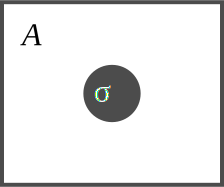
\includegraphics{sigma}
  \caption{Cross section probability}
  \label{fig:sigma}
\end{figure}
Assuming that an interaction will occur (with 100\% probability) if the projectile hits the solid, and not at all (0\% probability) if it misses, the total interaction probability for the single projectile will be
\begin{align}
  \label{eq:pssigma}
  P_S=\frac{\sigma}{A}\,.
\end{align}
Now suppose we have a parallel beam with density of particles $n$ and velocity $v$ towards the target. In time $t$, this beam fills a volume 
\begin{align}
  V=A v t\,.
\end{align}
Choosing $t$ such that the volume contains just one particle, we can write
\begin{align}
  n=1/V\,,
\end{align}
or
\begin{align}
  1=n v t A\,.
\end{align}
replacing back in \eqref{eq:pssigma} we have
\begin{align}
\sigma=\frac{P_s}{n v t}\,.  
\end{align}
$P_s$ is just the decay probability in eq.~\eqref{eq:w2}. Therefore
\begin{align}
  \sigma=\frac{\omega_2}{n v T}=&
\frac{1}{n v T}\int\ldots\int 
(2\pi)^4\delta^{(4)}\left(p_1+p_2-\sum_i k_j\right)VT 
\left|\mathcal{M}_{fi}\right|^2
\frac{1}{2E_{\mathbf{p}_1}V}\frac{1}{2E_{\mathbf{p}_2}V}
\prod_{j=1}^n\frac{d^3k_j}{(2\pi)^32E_{\mathbf{k}_j}}
\nonumber\\
=&\frac{1}{n v V}\int\ldots\int 
(2\pi)^4\delta^{(4)}\left(p_1+p_2-\sum_i k_j\right)
\left|\mathcal{M}_{fi}\right|^2
\frac{1}{2E_{\mathbf{p}_1}}\frac{1}{2E_{\mathbf{p}_2}}
\prod_{j=1}^n\frac{d^3k_j}{(2\pi)^32E_{\mathbf{k}_j}}\,.
\end{align}
The density of particles of the incident state is normalized to one particle  in the entire volume, so that $n=1/V$. Therefore
\begin{align}
   \sigma=&\frac{1}{v}\int\ldots\int 
(2\pi)^4\delta^{(4)}\left(p_1+p_2-\sum_i k_j\right)
\left|\mathcal{M}_{fi}\right|^2
\frac{1}{2E_{\mathbf{p}_1}}\frac{1}{2E_{\mathbf{p}_2}}
\prod_{j=1}^n\frac{d^3k_j}{(2\pi)^32E_{\mathbf{k}_j}}\,.
\end{align}
In general, as both particles may be moving we could use the relative velocity between them, $v_{\text{rel}}$,
\begin{align}
   \sigma=&\frac{1}{v_{\text{rel}}}\int\ldots\int 
(2\pi)^4\delta^{(4)}\left(p_1+p_2-\sum_i k_j\right)
\left|\mathcal{M}_{fi}\right|^2
\frac{1}{2E_{\mathbf{p}_1}}\frac{1}{2E_{\mathbf{p}_2}}
\prod_{j=1}^n\frac{d^3k_j}{(2\pi)^32E_{\mathbf{k}_j}}\,.
\end{align}
In a frame where $\mathbf{p}_1$ and $\mathbf{p}_2$ are along the same line, this reduces to
\begin{align}
  v_{\text{rel}}=\left|
    \frac{\mathbf{p}_1}{E_1}-\frac{\mathbf{p}_2}{E_2}
  \right|\,.
\end{align}
In fact, for not relativistic particles, where $E_i=m_i$, this coincides with the usual relative velocity
\begin{align}
   v_{\text{rel}}=&\left|
    \frac{m_1\mathbf{v}_1}{E_1}-\frac{m_2\mathbf{v}_2}{E_2}
  \right|\nonumber\\
=&\left|
    \mathbf{v}_1-\mathbf{v}_2
  \right|\,.
\end{align}
The most general formula for the relative velocity is 
\begin{align}
  v_{\text{rel}}=\frac{I}{E_1E_2}
\end{align}
where
\begin{align}
  I=&\sqrt{(p_1\cdot p_2)^2-m_1^2m_2^2}  
\end{align}

In general
\begin{align}
  I=&\sqrt{(E_1 E_2-\mathbf{p}_1\cdot\mathbf{p}_2)^2-m_1^2m_2^2}\nonumber\\
  =&\sqrt{E_1^2E_2^2+(\mathbf{p}_1\cdot\mathbf{p}_2)^2-2E_1 E_2\mathbf{p}_1.\mathbf{p}_2 -m_1^2m_2^2}
\end{align}

Since
\begin{align}
  m_1^2m_2^2=&(E_1^2-\mathbf{p}_1^2)(E_2^2-\mathbf{p}_2^2)\nonumber\\
=&(E_1^2E_2^2-\mathbf{p}_1^2E_2^2-E_1^2\mathbf{p}_2^2+\mathbf{p}_1^2\mathbf{p}_2^2)
\end{align}
\begin{align}
  I=\sqrt{\mathbf{p}_1^2E_2^2-2E_1 E_2\mathbf{p}_1\cdot\mathbf{p}_2+E_1^2\mathbf{p}_2^2
+(\mathbf{p}_1\cdot\mathbf{p}_2)^2-
\mathbf{p}_1^2\mathbf{p}_2^2}
\end{align}
If
\begin{align}
  (\mathbf{p}_1\cdot\mathbf{p}_2)^2-
\mathbf{p}_1^2\mathbf{p}_2^2=0
\end{align}
that implies that $\mathbf{p}_1$ and $\mathbf{p}_2$ are colineals,
\begin{align}
  I=&\sqrt{\mathbf{p}_1^2E_2^2-2E_1 E_2\mathbf{p}_1\cdot\mathbf{p}_2+E_1^2\mathbf{p}_2^2}
  \nonumber\\
  =&\sqrt{(\mathbf{p}_1E_2-\mathbf{p}_2E_1)^2}\nonumber\\
  =&|\mathbf{p}_1E_2-\mathbf{p}_2E_1|
\end{align}
\begin{align}
\label{eq:53}
v_{\text{rel}}=  \frac{I}{E_1E_2}=\left|
    \frac{\mathbf{p}_1}{E_1}-\frac{\mathbf{p}_2}{E_2}
  \right|
\end{align}


\begin{borrar}
Consider the collission of a cloud of particles of density $n_1^0$ moving to the right with velocity $v_1^0$ toward another cloud of particles in rest of density $n_2^0$. The differential of number of collisions is
\begin{align}
  d N\propto&|\mathbf{v}_1^0| n_1^0 n_2^0 \,d V\, dt\nonumber\\
  =&\sigma|\mathbf{v}_1^0| n_1^0 n_2^0 \,d V\, dt
\end{align}
Hence,  $\sigma$ have units of area, and corresponds to the cross section. 

The Lorentz invariant expression for velocities and particle densities is
\begin{align}
  |\mathbf{v}_1|^0 n_1^0 n_2^0\to n_1 n_2 \sqrt{(\mathbf{v}_1-\mathbf{v}_2)^2-(\mathbf{v}_1\times\mathbf{v}_2)^2}
\end{align}
Therefore
\begin{align}
  d N =&\sigma\sqrt{(\mathbf{v}_1-\mathbf{v}_2)^2-(\mathbf{v}_1\times\mathbf{v}_2)^2}n_1 n_2 \,d V\, dt  \nonumber\\
  =&\sigma\sqrt{(\mathbf{v}_1-\mathbf{v}_2)^2-(\mathbf{v}_1\times\mathbf{v}_2)^2}\frac{1}{V}(n_1V)(n_2 \,d V)\, dt\nonumber\\
 =&\sigma\sqrt{(\mathbf{v}_1-\mathbf{v}_2)^2-(\mathbf{v}_1\times\mathbf{v}_2)^2}\frac{1}{V}N_1(n_2 \,d V)\, dt\,.
\end{align}
Integrate it out
\begin{align}
  N=&\sigma\sqrt{(\mathbf{v}_1-\mathbf{v}_2)^2-(\mathbf{v}_1\times\mathbf{v}_2)^2}\frac{1}{V}N_1N_2 T
\end{align}
The probability for the collision to happens is
\begin{align}
  \label{eq:52}
  \frac{N}{N_1 N_2}=\frac{\sigma T}{V}\sqrt{(\mathbf{v}_1-\mathbf{v}_2)^2-(\mathbf{v}_1\times\mathbf{v}_2)^2}
\end{align}
The collision probability is according eq.~\eqref{eq:147}
\begin{align}
   \frac{N}{N_1 N_2}
=&\int\ldots\int 
(2\pi)^4\delta^{(4)}\left(p-\sum_i k_j\right)VT 
\left|\mathcal{M}_{fi}\right|^2
\frac{1}{2E_{\mathbf{p}_1}V}\frac{1}{2E_{\mathbf{p}_2}V}
\prod_{j=1}^n\frac{d^3k_j}{(2\pi)^32E_{\mathbf{k}_j}}
\end{align}
Replacing back in eq.~\eqref{eq:52}, we have that the  cross section is
\begin{align}
  \sigma=&\frac{V}{T\sqrt{(\mathbf{v}_1-\mathbf{v}_2)^2-(\mathbf{v}_1\times\mathbf{v}_2)^2}}\nonumber\\
&\times\int\ldots\int 
(2\pi)^4\delta^{(4)}\left(p_1+p_2-\sum_i k_j\right)VT 
\left|\mathcal{M}_{fi}\right|^2
\frac{1}{2E_{\mathbf{p}_1}V}\frac{1}{2E_{\mathbf{p}_2}V}
\prod_{j=1}^n\frac{d^3k_j}{(2\pi)^32E_{\mathbf{k}_j}}
\end{align}
Defining
\begin{align}
  I=E_{\mathbf{p}_1} E_{\mathbf{p}_2} \sqrt{(\mathbf{v}_1-\mathbf{v}_2)^2-(\mathbf{v}_1\times\mathbf{v}_2)^2}
\end{align}
we have the differential cross section as
\begin{align}
  d\sigma=&\frac{V E_{\mathbf{p}_1} E_{\mathbf{p}_2} }{T I}
(2\pi)^4\delta^{(4)}\left(p_1+p_2-\sum_i k_j\right)VT 
\left|\mathcal{M}_{fi}\right|^2
\frac{1}{2E_{\mathbf{p}_1}V}\frac{1}{2E_{\mathbf{p}_2}V}
\prod_{j=1}^n\frac{d^3k_j}{(2\pi)^32E_{\mathbf{k}_j}}
\end{align}
In this way, when the initial state in the $S$--matrix contains two particles
\begin{align}
  d\sigma=(2\pi)^4\delta^{(4)}\left(\sum_{i=1,2} p_i-\sum_{j}k_j\right)
\frac{1}{4I}\left|\mathcal{M}_{fi}\right|^2
\prod_{j}\frac{d^3k_j}{(2\pi)^32E_{\mathbf{k}_j}}
\end{align}
where
\begin{align}
  I=&\sqrt{(p_1\cdot p_2)^2-m_1^2m_2^2}\nonumber\\
=&E_{\mathbf{p}_1} E_{\mathbf{p}_2} \sqrt{(\mathbf{v}_1-\mathbf{v}_2)^2-(\mathbf{v}_1\times\mathbf{v}_2)^2}
\end{align}
Defining 
\begin{align}
  v_{\text{rel}}=\frac{I}{E_1E_2}
\end{align}
In general
\begin{align}
  I=&\sqrt{(E_1 E_2-\mathbf{p}_1\cdot\mathbf{p}_2)^2-m_1^2m_2^2}\nonumber\\
  =&\sqrt{E_1^2E_2^2+(\mathbf{p}_1\cdot\mathbf{p}_2)^2-2E_1 E_2\mathbf{p}_1.\mathbf{p}_2 -m_1^2m_2^2}
\end{align}

Since
\begin{align}
  m_1^2m_2^2=&(E_1^2-\mathbf{p}_1^2)(E_2^2-\mathbf{p}_2^2)\nonumber\\
=&(E_1^2E_2^2-\mathbf{p}_1^2E_2^2-E_1^2\mathbf{p}_2^2+\mathbf{p}_1^2\mathbf{p}_2^2)
\end{align}
\begin{align}
  I=\sqrt{\mathbf{p}_1^2E_2^2-2E_1 E_2\mathbf{p}_1\cdot\mathbf{p}_2+E_1^2\mathbf{p}_2^2
+(\mathbf{p}_1\cdot\mathbf{p}_2)^2-
\mathbf{p}_1^2\mathbf{p}_2^2}
\end{align}
If
\begin{align}
  (\mathbf{p}_1\cdot\mathbf{p}_2)^2-
\mathbf{p}_1^2\mathbf{p}_2^2=0
\end{align}
that implies that $\mathbf{p}_1$ and $\mathbf{p}_2$ are colineals,
\begin{align}
  I=&\sqrt{\mathbf{p}_1^2E_2^2-2E_1 E_2\mathbf{p}_1\cdot\mathbf{p}_2+E_1^2\mathbf{p}_2^2}
  \nonumber\\
  =&\sqrt{(\mathbf{p}_1E_2-\mathbf{p}_2E_1)^2}\nonumber\\
  =&|\mathbf{p}_1E_2-\mathbf{p}_2E_1|
\end{align}
\begin{align}
\label{eq:53}
v_{\text{rel}}=  \frac{I}{E_1E_2}=\left|
    \frac{\mathbf{p}_1}{E_1}-\frac{\mathbf{p}_2}{E_2}
  \right|
\end{align}
\end{borrar}
To simplify the notation we set $E_i=E_{\mathbf{p}_i}=$, and $E_f=E_{\mathbf{p}_f}$. Moreover, the differential cross section is
\begin{align}
    d\sigma=&(2\pi)^4\delta^{(4)}\left(\sum_{i=1}^2p_i-\sum_{f} p_f\right)
\frac{1}{4v_{\text{rel}}E_1E_2}\left|\mathcal{M}_{fi}\right|^2
\prod_{f}\frac{d^3k_f}{(2\pi)^32E_{f}}\nonumber\\
&=(2\pi)^4\frac{1}{4v_{\text{rel}}E_1E_2}\left|\mathcal{M}_{fi}\right|^2
d\Phi^{n}(p_1,p_2;k_1,\ldots,k_n)
\end{align}
where
\begin{align}
  \label{eq:50}
    d \Phi^{(n)} (p_1,p_2; k_1, k_2,\dots, k_n) = \delta^{(4)}\left(p-\sum_j k_j\right)  \prod_{j=1}^n \frac{d^3 k_j}{(2\pi)^3 2 E_{\mathbf{k}_j}} \,.
\end{align}
We keep the diferential notation both for $d\sigma$, and $d\Phi$ until the last integration have been made.

\subsection{2--to--2 cross section}
\label{sec:2-2-cross}

The the 2--to--2 cross section is
\begin{align}
 \label{eq:54}
  d\sigma=&\frac{(2\pi)^4}{4v_{\text{rel}}E_1E_2}\left|\mathcal{M}_{fi}\right|^2
d\Phi^{2}(p_1,p_2;p'_1,p'_2)\nonumber\\
=&\frac{2^4\pi^4}{2^{8}\pi^64v_{\text{rel}}E_1E_2}2^{8}\pi^6\left|\mathcal{M}_{fi}\right|^2
d\Phi^{n}(p_1,p_2;k_1,\ldots,k_n)\nonumber\\
=&\frac{1}{2^{6}\pi^2v_{\text{rel}}E_1E_2}\left|\mathcal{M}_{fi}\right|^2
\left[4(2\pi)^6d\Phi^{2}(p_1,p_2;p'_1,p'_2)\right]\nonumber\\
=&\frac{1}{64\pi^2v_{\text{rel}}E_1E_2}\left|\mathcal{M}_{fi}\right|^2
\left[4(2\pi)^6d\Phi^{2}(p_1,p_2;p'_1,p'_2)\right]
\end{align}
where, as in eq.~\eqref{eq:50}
\begin{align}
4(4\pi)^6d\Phi^{(2)}(p_1,p_2;p_1',p_2')&= \frac{4(4\pi)^6}{4(2\pi)^6} \delta^{(4)}\left(p_1+p_2-p_1'-p_2'\right)
\frac{d^3p_1'}{E_{1}'}\frac{d^3p_2'}{E_{2}'}\nonumber\\
&=  \delta^{(4)}\left(p_1+p_2-p_1'-p_2'\right)4(2\pi)^6
\frac{d^3p_1'}{E_{1}'}\frac{d^3p_2'}{E_{2}'}
\end{align}
We now will find an expression for cross section in the center of mass frame (CM) 


The center of mass (CM) frame is defined by the condition
\begin{align}
  \label{eq:cm}
  \mathbf{p}_1+\mathbf{p}_2=0
\end{align}


The $\delta$--function in Eq.~\eqref{eq:101}
\begin{align}
\label{eq:56}
  \delta^{(4)}(p+p_2-p_1'-p_2')=\delta^{(3)}(\mathbf{p}_1+\mathbf{p}_2-\mathbf{p}_1'-\mathbf{p}_2')
\delta(E_1+E_2-E_1'-E_2')
\end{align}
In the CM frame
\begin{align}
\label{eq:148}
  \delta^{(4)}(p+p_2-p_1'-p_2')=\delta^{(3)}(\mathbf{p}_1'+\mathbf{p}_2')
\delta(E_1+E_2-E_1'-E_2')
\end{align}
$\mathcal{M}_{fi}$ in integration does not depend on $|\mathbf{p}_1'|$ or $|\mathbf{p}_2'|$ as the final momentum is fixed by the initial momentum whenever the final states have only two particles. In this way the integration on $p_2'$ can be evaluated directly for $d\Phi^{(2)}$. Replacing back in Eq.~\eqref{eq:54}
\begin{align}
\label{eq:149}
  4(2\pi)^6d\Phi^{(2)}=&\delta^{(3)}(\mathbf{p}_1'+\mathbf{p}_2')\delta(E_1+E_2-E_1'-E_2')
\frac{d^3p_1'}{E_{1}'}\frac{d^3p_2'}{E_{2}'}\nonumber\\
 =&\delta(E_1+E_2-E_1'-E_2')
\frac{d^3p_1'}{E_{1}'}\int\delta^{(3)}(\mathbf{p}_1'+\mathbf{p}_2')\frac{d^3p_2'}{E_{2}'}\nonumber\\
=&\delta(E_1+E_2-E_1'-E_2')
\frac{d^3p_1'}{E_{1}'E_{2}'}
\end{align}

\begin{align}
  4(2\pi)^6d\Phi^{(2)}=\delta(E_1+E_2-E_1'-E_2')
  \frac{{\mathbf{p}_1'}^2d|\mathbf{p}_1'|d\Omega}{E_{1}'E_{2}'}
\end{align}

As
\begin{align}
  |\mathbf{p}_1'|=\sqrt{{E_1'}^2-{m_1}^2}
\end{align}

\begin{align}
  \frac{d|\mathbf{p}_1'|}{dE_1'}=&\frac{2E_1'}{2\sqrt{{E_1'}^2-{m_1}^2}}\nonumber\\
  =&\frac{E_1'}{|\mathbf{p}_1'|}
\end{align}
In this way, we can write, in general
\begin{align}
 |\mathbf{p}|\, d|\mathbf{p}|=E\,dE
\end{align}
and
\begin{align}
\label{eq:57}
 4(2\pi)^6 d\Phi^{(2)}&=\delta(E_1+E_2-E_1'-E_2')
\frac{|\mathbf{p}_1'|E_1'dE_1'}{E_{1}'E_{2}'}d\Omega\nonumber\\
  &=\delta(E_1+E_2-E_1'-E_2')
\frac{|\mathbf{p}_1'|dE_1'}{E_{2}'}d\Omega
\end{align}
From the $\delta$--function in Eq.~\eqref{eq:56} we have that in the CM frame
\begin{align}
  \mathbf{p}_1+\mathbf{p}_2-\mathbf{p}_1'-\mathbf{p}_2'=0 \overset{\text{CM}}{\Rightarrow}
  \begin{cases}
    \mathbf{p}_1=-\mathbf{p}_2\\
    \mathbf{p}_1'=-\mathbf{p}_2'\\
  \end{cases}
\end{align}

Squaring the first expression, and taking into account that
\begin{align}
  \label{eq:58}
  {\mathbf{p}'_1}= \sqrt{{E_1'}^2-{m_1'}^2}
\end{align}
we have
\begin{align}
  {\mathbf{p}'_1}^2=&{\mathbf{p}'_2}^2\nonumber\\
  {E_1'}^2-{m_1'}^2=&  {E_2'}^2-{m_2'}^2\,,
\end{align}
\begin{align}
\label{eq:59}
  E_2'=\sqrt{{E_1'}^2-{m_1'}^2+{m_2'}^2}
\end{align}
In this way we can express $E_2'$ in terms of $E_1'$ in Eq.~\eqref{eq:57}.
Moreover, we can define the center of mass energy as
\begin{align}
\label{eq:smv}
  s=&\left( p_1+p_2 \right)^2\,.
\end{align}

By using the center of mass condition \eqref{eq:cm}
\begin{align}
  \mathbf{p}=\mathbf{p}_1=-\mathbf{p}_2\,,
\end{align}
then
\begin{align}
   s=& p_1^2+p_2^2+2 p_1\cdot p_2 \nonumber\\
=&  p_1^2+p_2^2+2  \left( E_1 E_2-\mathbf{p}_1\cdot\mathbf{p}_2 \right)\nonumber\\
=& p_1^2+p_2^2+2\left( E_1 E_2+\mathbf{p}_1^2 \right) \nonumber\\
=& p_1^2+p_2^2+2\left( E_1 E_2+ E_1^2-p_1^2 \right) \nonumber\\
=& p_1^2+p_2^2+2\left( E_1 E_2+ E_1^2-p_1^2 \right) \nonumber\\
=& p_2^2-p_1^2+2\left( E_1 E_2+ E_1^2 \right) \nonumber\\
=& E_2^2-\mathbf{p}_1^2-E_2^2+\mathbf{p}_2^2+2\left( E_1 E_2+ E_1^2 \right) \nonumber\\
=& E_2^2-E_1^2+2\left( E_1 E_2+ E_1^2 \right) \nonumber\\
=& E_1^2 +2E_1 E_2+ E_2^2 \nonumber\\
=& \left( E_1+E_2 \right)^2\,.
\end{align}
So that
\begin{align}
  \label{eq:60}
  \sqrt{s}=E_1+E_2
\end{align}
Using The energy part of $\delta$--function in Eq.~\eqref{eq:56} can be written as
\begin{align}
  \delta\left(\sqrt{s}-E_1'-\sqrt{{E_1'}^2-{m_1'}^2+{m_2'}^2}\right)
\end{align}
As established before,  $\mathcal{M}_{fi}$ in this case in independent of $|\mathbf{p}'_1|$, and the integration on $E_1'$ can be done directly only for $d\Phi^{(2)}$.
The integral is easily performed using the identity
\begin{align}
  \delta\left(f(z)\right)=\sum_n\frac{\delta(z-z_n)}{|f'(z_n)|}
\end{align}
where $z_n$ are the zeroes of $f(z)$. In this case, this $\delta$--function is a function of the integration variable $E_1'$, with only one zero
\begin{align}
   \delta\left(f(x)\right)=\frac{\delta(x-x_0)}{|f'(x_0)|}
\end{align}
where
\begin{align}
  f(x)=\sqrt{s}-x-\sqrt{x^2-{m_1'}^2+{m_2'}^2}
\end{align}
Therefore
\begin{align}
  \label{eq:61}
   4(2\pi)^6d\Phi^{(2)}=&d\Omega\int\frac{\delta(x-x_0)}{|f'(x_0)|}\frac{
     |\mathbf{p}_1'(x)|}{E_2'(x)}dx\nonumber\\
   =&d\Omega\frac{1}{|f'(x_0)|}\frac{
     |\mathbf{p}_1'(x_0)|}{E_2'(x_0)}\nonumber\\
\end{align}
where from Eqs.~\eqref{eq:58}, \eqref{eq:59},
\begin{align}
  \label{eq:62}
  \mathbf{p}_1'(x_0)=&\sqrt{x_0^2-{m_1'}^2}&
  E_2'(x_0)=&\sqrt{x_0^2-{m_1'}^2+{m_2'}^2}
\end{align}
The zero is obtained from
\begin{align}
  &\sqrt{s}-x_0-\sqrt{x_0^2-{m_1'}^2+{m_2'}^2}=0\nonumber\\
  &s-2\sqrt{s}\,x_0+x_0^2=x_0^2-{m_1'}^2+{m_2'}^2\nonumber\\
  &s-2\sqrt{s}\,x_0=-{m_1'}^2+{m_2'}^2
\end{align}
with solution
\begin{align}
  \label{eq:63}
  x_0=\frac{s+{m_1'}^2-{m_2'}^2}{2\sqrt{s}}
\end{align}
As (See 
\texttt{deltaxn.nb} %noinstiki [deltax.nb](Appendix)
for additional details)
\begin{align}
  f'(x)=-\frac{x}{\sqrt{x^2-{m_1'}^2+{m_2'}^2}}-1
\end{align}
we have
\begin{align}
  \label{eq:64}
  f'(x_0)=&-\frac{{m_1'}^2-{m_2'}^2+s}{\sqrt{s}
   \sqrt{\frac{\left(-{m_1'}^2+{m_2'}^2+s\right)^2}{s}}}-1\nonumber\\
    =&\frac{-{m_1'}^2+{m_2'}^2-s}{-{m_1'}^2+{m_2'}^2+s}-1\nonumber\\
    =&\frac{-{m_1'}^2+{m_2'}^2-s+{m_1'}^2-{m_2'}^2-s}{-{m_1'}^2+{m_2'}^2+s}\nonumber\\
=&\frac{-2s}{s+{m_2'}^2-{m_1'}^2}\,,
\end{align}
and
\begin{align}
  \label{eq:65}
  \delta(f(E_1'))=\delta(E_1'-x_0)\left(\frac{s+{m_2'}^2-{m_1'}^2}{2s}\right)
\end{align}

Replacing the expression for $x_0$ in \eqref{eq:63} into Eq.~\eqref{eq:62} we have (See 
\texttt{deltaxn.nb}  %noinstiki [deltax.nb](Appendix)
for additional details)
\begin{align}
  \label{eq:66}
   |\mathbf{p}_1'(x_0)|=&\frac{\sqrt{[s-({m_1'}-{m_2'})^2][s-({m_1'}+{m_2'})^2]}}{2\sqrt{s}}\nonumber\\
E_2'(x_0)=&  \frac{s-{m_1'}^2+{m_2'}^2}{2\sqrt{s}}
\end{align}

Replacing Eqs.~\eqref{eq:64}, and \eqref{eq:66} in Eq.~\eqref{eq:61}
we have
\begin{align}
  \label{eq:67}
4(2\pi)^6d\Phi^{(2)}&=d\Omega\frac{1}{|f'(x_0)|}
\frac{\sqrt{x_0^2-{m_1'}^2}}{\sqrt{x_0^2-{m_1'}^2+{m_2'}^2}}\nonumber\\
  &=d\Omega\left(\frac{s-{m_1'}^2+{m_2'}^2}{2s}\right)
\frac{\sqrt{[s-({m_1'}-{m_2'})^2][s-({m_1'}+{m_2'})^2]}}{s-{m_1'}^2+{m_2'}^2}\nonumber\\
&=d\Omega\frac{\sqrt{[s-({m_1'}-{m_2'})^2][s-({m_1'}+{m_2'})^2]}}{2s}
\end{align}
Defining the kinematic two particle function
\begin{align}
  \label{eq:46}
  \lambda(a,b,c)\equiv(a-b+c)^2-4ac
\end{align}
and taking into account that
\begin{align}
  \left(s-{m_2'}^2+{m_1'}^2\right)^2-4s{m_1'}^2=[s-({m_1'}-{m_2'})^2][s-({m_1'}+{m_2'})^2]
\end{align}
we have
\begin{align}
\label{eq:150}
  4(2\pi)^6d\Phi^{(2)}=d\Omega\frac{\lambda^{1/2}(s,{m_2'}^2,{m_1'}^2)}{2s}
\end{align}
Moreover
\begin{align}
  \label{eq:151}
  \mathbf{p}_1'=&\frac{\lambda^{1/2}(s,{m_2'}^2,{m_1'}^2)}{2\sqrt{s}}
\end{align}
%\left(\right)

To further evaluate Eq.~(\ref{eq:54}), we need to express $v_{\text{rel}}$ and $E_1E_2$ in terms of $s$ and the masses. Concerning $v_{\text{rel}}$,
from Eq.~\eqref{eq:53}, evaluated in CM frame
\begin{align}
  \label{eq:68}
    E_1E_2 v_{\text{rel}}=&E_1E_2\left|\frac{\mathbf{p}_1}{E_1}-\frac{\mathbf{p}_2}{E_2}\right|\nonumber\\
  =&E_1E_2\left|\frac{\mathbf{p}_1}{E_1}+\frac{\mathbf{p}_1}{E_2}\right|\nonumber\\
  =&\left|\mathbf{p}_1\right|({E_1+E_2})\nonumber\\
  =&\left|\mathbf{p}_1\right|\sqrt{s}
\end{align}
Replacing back Eqs.~\eqref{eq:67}, and \eqref{eq:68} into Eq.~\eqref{eq:54}, we have
\begin{align}
  \label{eq:69}
      d\sigma=&\frac{1}{64\pi^2E_1E_2v_{\text{rel}}}\overline{\left|\mathcal{M}_{fi}\right|^2}
    \left[4(2\pi)^6d\Phi^{(2)}\right]
\end{align}
\begin{align}
  \frac{d\sigma}{d\Omega}=\frac{1}{64\pi^2E_1E_2v_{\text{rel}}}\overline{\left|\mathcal{M}_{fi}\right|^2}
\frac{\sqrt{[s-({m_1'}+{m_2'})^2][s-({m_1'}-{m_2'})^2]}}{2s}
\end{align}
By using Eq.~\eqref{eq:68}
\begin{align}
  \frac{d\sigma}{d\Omega}=\frac{1}{64\pi^2|\mathbf{p}_1|\sqrt{s}}\overline{\left|\mathcal{M}_{fi}\right|^2}
\frac{\sqrt{[s-({m_1'}+{m_2'})][s-({m_1'}^2-{m_2'}^2)]}}{2s}
\end{align}
In the CM frame
\begin{align}
\sqrt{s}=&E_1+E_2\nonumber\\
=&\sqrt{\mathbf{p}_1^2+m_1^2}+\sqrt{\mathbf{p}_2^2+m_2^2}\nonumber\\
=&\sqrt{\mathbf{p}_1^2+m_1^2}+\sqrt{\mathbf{p}_1^2+m_2^2}
\end{align}

\begin{align}
  \label{eq:70}
  s=&2\mathbf{p}_1^2+m_1^2+m_2^2+2\sqrt{\mathbf{p}_1^4+(m_1^2+m_2^2)\mathbf{p}_1^2+m_1^2m_2^2}\nonumber\\
s-(2\mathbf{p}_1^2+m_1^2+m_2^2)=&2\sqrt{\mathbf{p}_1^4+(m_1^2+m_2^2)\mathbf{p}_1^2+m_1^2m_2^2}
\end{align}
\begin{align}
  s^2-2s(2\mathbf{p}_1^2+m_1^2+m_2^2)+[2\mathbf{p}_1^2+(m_1^2+m_2^2)]^2=&4(\mathbf{p}_1^4+(m_1^2+m_2^2)\mathbf{p}_1^2+m_1^2m_2^2)\nonumber\\
  s^2-2s(2\mathbf{p}_1^2+m_1^2+m_2^2)+4\mathbf{p}_1^4+4\mathbf{p}_1^2(m_1^2+m_2^2)
+(m_1^2+m_2^2)^2=&4(\mathbf{p}_1^4+(m_1^2+m_2^2)\mathbf{p}_1^2+m_1^2m_2^2)\nonumber\\
-4s\mathbf{p}_1^2+s^2-2s(m_1^2+m_2^2)+(m_1^2+m_2^2)^2=&4m_1^2m_2^2\nonumber\\
-4s\mathbf{p}_1^2+s^2-2sm_1^2-2sm_2^2+m_1^4+m_2^4+2m_1^2m_2^2=&4m_1^2m_2^2\nonumber\\
-4s\mathbf{p}_1^2+s^2-2sm_1^2-2sm_2^2+m_1^4+m_2^4-2m_1^2m_2^2=&0
\end{align}
\begin{align}
  \mathbf{p}_1^2=\frac{\left(s-m_1^2-2 m_2 m_1-m_2^2\right)
   \left(s-m_1^2+2 m_2m_1-m_2^2\right)}
{4s}
\end{align}
\begin{align}
  \label{eq:71}
  |\mathbf{p}_1|=&\frac{\sqrt{[s-(m_1+m_2)^2][s-(m_1-m_2)^2]}}{2\sqrt{s}}\nonumber\\
=&\frac{\lambda^{1/2}(s,m_2^2,m_1^2)}{2\sqrt{s}}
\end{align}
Replacing Eq.~\eqref{eq:71} back in Eq.~\eqref{eq:68} we have
\begin{align}
  \label{eq:72}
  E_1E_2 v_{\text{rel}}=\frac{1}{2}\sqrt{[s-(m_1+m_2)^2][s-(m_1-m_2)^2]}
\end{align}
Replacing Eqs.~\eqref{eq:72}, and \eqref{eq:67} in Eq.~\eqref{eq:54}
\begin{align}
  \label{eq:73}
  d\sigma=&\frac{1}{64\pi^2}\overline{\left|\mathcal{M}_{fi}\right|^2}\frac{d\Omega}{2s}(2)
\sqrt{\frac{[s-(m_1'+m_2')^2][s-(m_1'-m_2')^2]}{[s-(m_1+m_2)^2][s-(m_1-m_2)^2]}}
\end{align}
and, finally
\begin{align}
  \frac{d\sigma}{d\Omega}=\frac{1}{64\pi^2s}\left\{
\frac{[s-(m_1'+m_2')^2][s-(m_1'-m_2')^2]}{[s-(m_1+m_2)^2][s-(m_1-m_2)^2]}\right\}^{1/2}
\overline{|\mathcal{M}|^2}
\end{align}
or, in terms of the kinematic function defined in eq.~\eqref{eq:46}
\begin{align}
  \label{eq:2bcs}
  \frac{d\sigma}{d\Omega}=\frac{1}{64\pi^2s}
\frac{\lambda^{1/2}(s,{m_2'}^2,{m_1'}^2)}{\lambda^{1/2}(s,m_2^2,m_1^2)}
\overline{|\mathcal{M}|^2}
\end{align}
%\left(\right)

\section{Decay Rates}
\label{sec:decay-rates}
Consider the matrix element of $i T$ in (\ref{eq:41})
\begin{align}
  \label{eq:45}
  \langle\mathbf{k}_1\ldots\mathbf{k}_n|i T|\mathbf{p}\rangle^{\text{NR}}=(2\pi)^4\delta^{(4)}\left(p-\sum_i k_i\right)i{M}_{fi}
\end{align}

where the initial state is a single particle of momentum $p$ and mass $M$, while the final state is given by $n$ particles of momenta $k_i$ and masses $m_i$, $i=1,\ldots,n$. 
We are therefore considering a decay process. 


By using eq.~\eqref{eq:146} we have
\begin{align}
\omega=&\int\ldots\int 
(2\pi)^4\delta^{(4)}\left(p-\sum_i k_j\right)\left(\int dt\right) 
\left|\mathcal{M}_{fi}\right|^2
\frac{1}{2E_{\mathbf{p}}}
\prod_{j=1}^n\frac{d^3k_j}{(2\pi)^32E_{\mathbf{k}_j}}
\end{align}
Therefore the differential probability is
\begin{align}
  d\omega=&
(2\pi)^4\delta^{(4)}\left(p-\sum_i k_j\right)
\frac{1}{2E_{\mathbf{p}}}\left|\mathcal{M}_{fi}\right|^2
dt\prod_{j=1}^n\frac{d^3k_j}{(2\pi)^32E_{\mathbf{k}_j}}
\end{align}
Finally we define the \textit{decay rate} $d\Gamma$ as the decay probability in which in the final state
the j--th particle has momentum between $k_j$ and $k_j+ dk_j$ per unit time
\begin{align}
\label{eq:49}
d\Gamma\equiv&\frac{d\omega}{dt}=
(2\pi)^4\delta^{(4)}\left(p-\sum_j k_j\right)
\frac{1}{2E_{\mathbf{p}}}\left|\mathcal{M}_{fi}\right|^2
\prod_{j=1}^n\frac{d^3k_j}{(2\pi)^32E_{\mathbf{k}_j}}\nonumber\\
=&\frac{(2\pi)^4}{2E_{\mathbf{p}}}\left|\mathcal{M}_{fi}\right|^2
d \Phi^{(n)} (p; k_1, k_2,\dots, k_n)
\end{align}
where
\begin{align}
  \label{eq:50}
    d \Phi^{(n)} (p; k_1, k_2,\dots, k_n) = \delta^{(4)}\left(p-\sum_j k_j\right)  \prod_{j=1}^n \frac{d^3 k_j}{(2\pi)^3 2 E_{\mathbf{k}_j}} \,.
\end{align}
and the differential decay width in the center of mass frame
\begin{align}
  \label{eq:51}
  d\Gamma=\frac{(2\pi)^4}{2E_{\mathbf{p}}}\left|\mathcal{M}_{fi}\right|^2
d \Phi^{(n)} (p; k_1, k_2,\dots, k_n)
\end{align}


\subsection{Two body decays}
We now consider the decay of particle of mass $M$ decaying into two particles of 4--momenta $p_1$, $p_2$ and masses $m_1$, $m_2$. In the CM frame the initial momentum satisfy
\begin{align}
  \mathbf{p}=&0\Rightarrow M=E_{\mathbf{p}}
\end{align}
Therefore 
\begin{align}
  \label{eq:51nn}
  d\Gamma=&\frac{(2\pi)^4}{2M[4(2\pi)^6]}\left|\mathcal{M}_{fi}\right|^2
4(2\pi)^6d \Phi^{(2)} (p; p_1, p_2)\nonumber\\
=&\frac{1}{2^3M(2\pi)^2}\left|\mathcal{M}_{fi}\right|^2
4(2\pi)^6d \Phi^{(2)} (p; p_1, p_2)\nonumber\\
=&\frac{1}{32 \pi^2M}\left|\mathcal{M}_{fi}\right|^2
\left[4(2\pi)^6d \Phi^{(2)} (p; p_1, p_2)\right]
\end{align}
where
\begin{align}
  4(2\pi)^6d \Phi^{(2)} (p; p_1, p_2)=\delta^{(4)}(p-p_1-p_2)\frac{d^3p_1}{E_{1}}\frac{d^3p_2}{E_{2}}
\end{align}
The Dirac delta in eq.~\eqref{eq:50} can be written in the CM frame as
\begin{align}
\label{eq:153}
  \delta^{(4)}(p-p_1-p_2)=&\delta^{(3)}(\mathbf{p}-\mathbf{p}_1-\mathbf{p}_2)\delta(E-E_1-E_2)\nonumber\\
=&\delta^{(3)}(\mathbf{p}_1+\mathbf{p}_2)\delta(M-E_1-E_2)
\end{align}
and,
\begin{align}
   4(2\pi)^6d \Phi^{(2)} (p; p_1, p_2)=&\delta(M-E_1-E_2)\delta^{(3)}(\mathbf{p}_1+\mathbf{p}_2)\frac{d^3p_1}{E_{1}}\frac{d^3p_2}{E_{2}}
\end{align}
We now proceed  with a calculation similat to the one leading to eq.~\eqref{eq:149} \footnote{ we see that the two quantities are the same after the replacing $\sqrt{s}\to M$, $p_1'\to p_1$ and $p_2'\to p_2$.} 
\begin{align}
\label{eq:149nn}
  4(2\pi)^6d\Phi^{(2)}=&\delta^{(3)}(\mathbf{p}_1+\mathbf{p}_2)\delta(M-E_1-E_2)
\frac{d^3p_1}{E_{1}}\frac{d^3p_2}{E_{2}}\nonumber\\
 =&\delta(M-E_1-E_2)
\frac{d^3p_1}{E_{1}}\int\delta^{(3)}(\mathbf{p}_1+\mathbf{p}_2)\frac{d^3p_2}{E_{2}}\nonumber\\
=&\delta(M-E_1-E_2)
\frac{d^3p_1}{E_{1}E_{2}}
\end{align}

\begin{align}
  4(2\pi)^6d\Phi^{(2)}=\delta(M-E_1-E_2)
  \frac{{\mathbf{p}_1}^2d|\mathbf{p}_1|d\Omega}{E_{1}E_{2}}
\end{align}

As
\begin{align}
  |\mathbf{p}_1|=\sqrt{{E_1}^2-{m_1}^2}
\end{align}

\begin{align}
  \frac{d|\mathbf{p}_1|}{dE_1}=&\frac{2E_1}{2\sqrt{{E_1}^2-{m_1}^2}}\nonumber\\
  =&\frac{E_1}{|\mathbf{p}_1|}
\end{align}
In this way, we can write, in general
\begin{align}
 |\mathbf{p}|\, d|\mathbf{p}|=E\,dE
\end{align}
and
\begin{align}
 4(2\pi)^6 d\Phi^{(2)}&=\delta(M-E_1-E_2)
\frac{|\mathbf{p}_1|E_1dE_1}{E_{1}E_{2}}d\Omega\nonumber\\
  &=\delta(M-E_1-E_2)
\frac{|\mathbf{p}_1|dE_1}{E_{2}}d\Omega
\end{align}
From the $\delta$--function in Eq.~\eqref{eq:56} we have that in the CM frame
\begin{align}
 \mathbf{p}_1-\mathbf{p}_2=0 \overset{\text{CM}}{\Rightarrow}
    \mathbf{p}_1=-\mathbf{p}_2
\end{align}

Squaring the first expression, and taking into account that
\begin{align}
  {\mathbf{p}_1}= \sqrt{{E_1}^2-{m_1}^2}
\end{align}
we have
\begin{align}
  {\mathbf{p}_1}^2=&{\mathbf{p}_2}^2\nonumber\\
  {E_1}^2-{m_1}^2=&  {E_2}^2-{m_2}^2\,,
\end{align}
\begin{align}
  E_2=\sqrt{{E_1}^2-{m_1}^2+{m_2}^2}
\end{align}
In this way we can express $E_2$ in terms of $E_1$ in Eq.~\eqref{eq:57}.

Using The energy part of $\delta$--function in Eq.~\eqref{eq:56} can be written as
\begin{align}
  \delta\left(M-E_1-\sqrt{{E_1}^2-{m_1}^2+{m_2}^2}\right)
\end{align}
As established before,  $\mathcal{M}_{fi}$ in this case in independent of $|\mathbf{p}_1|$, and the integration on $E_1$ can be done directly only for $d\Phi^{(2)}$.

The integral is easily performed using the identity
\begin{align}
   \delta\left(f(x)\right)=\frac{\delta(x-x_0)}{|f'(x_0)|}
\end{align}
where
\begin{align}
  f(x)=M-x-\sqrt{x^2-{m_1}^2+{m_2}^2}
\end{align}
and the root is given by~\eqref{eq:63}
\begin{align}
  x_0=\frac{M^2+{m_1}^2-{m_2}^2}{2M}
\end{align}

Therefore
\begin{align}
  \label{eq:61nn}
   4(2\pi)^6d\Phi^{(2)}=&d\Omega\int\frac{\delta(x-x_0)}{|f'(x_0)|}\frac{
     |\mathbf{p}_1(x)|}{E_2(x)}dx\nonumber\\
   =&d\Omega\frac{1}{|f'(x_0)|}\frac{
     |\mathbf{p}_1(x_0)|}{E_2(x_0)}\,,
\end{align}
where 
\begin{align}
  \label{eq:62nn}
  \mathbf{p}_1(x_0)=&\sqrt{x_0^2-{m_1}^2}&
  E_2(x_0)=&\sqrt{x_0^2-{m_1}^2+{m_2}^2}
\end{align}

As (See 
\texttt{deltaxn.nb} %noinstiki [deltax.nb](Appendix)
for additional details)
\begin{align}
  f'(x)=-\frac{x}{\sqrt{x^2-{m_1}^2+{m_2}^2}}-1
\end{align}
we have as in~\eqref{eq:64}
\begin{align}
  \label{eq:64nn}
  f'(x_0)=&\frac{-2M^2}{M^2+{m_2}^2-{m_1}^2}\,,
\end{align}
and
\begin{align}
  \label{eq:65nn}
  \delta(f(E_1))=\delta(E_1-x_0)\left(\frac{M^2+{m_2}^2-{m_1}^2}{2M^2}\right)
\end{align}

Replacing the expression for $x_0$ in into Eq.~\eqref{eq:62nn} we have (See 
\texttt{deltaxn.nb}  %noinstiki [deltax.nb](Appendix)
for additional details)
\begin{align}
  \label{eq:66nn}
  |\mathbf{p}_1(x_0)|=&\frac{\sqrt{[M^2-({m_1}-{m_2})^2][M^2-({m_1}+{m_2})^2]}}{2M}\nonumber\\
E_2(x_0)=&  \frac{M^2-{m_1}^2+{m_2}^2}{2M}
\end{align}

Replacing Eqs.~\eqref{eq:64nn}, and \eqref{eq:66nn} in Eq.~\eqref{eq:61nn}
we have
\begin{align}
  \label{eq:67nn}
4(2\pi)^6d\Phi^{(2)}&=d\Omega\frac{1}{|f'(x_0)|}
\frac{\sqrt{x_0^2-{m_1}^2}}{\sqrt{x_0^2-{m_1}^2+{m_2}^2}}\nonumber\\
  &=d\Omega\left(\frac{M^2-{m_1}^2+{m_2}^2}{2M^2}\right)
\frac{\sqrt{[M^2-({m_1}-{m_2})^2][M^2-({m_1}+{m_2})^2]}}{M^2-{m_1}^2+{m_2}^2}\nonumber\\
&=d\Omega\frac{\sqrt{[M^2-({m_1}-{m_2})^2][M^2-({m_1}+{m_2})^2]}}{2M^2}
\end{align}
Defining the kinematic two particle function
\begin{align}
  \label{eq:46}
  \lambda(a,b,c)\equiv(a-b+c)^2-4ac
\end{align}
and taking into account that
\begin{align}
  \left(M^2-{m_2}^2+{m_1}^2\right)^2-4M^2{m_1}^2=[M^2-({m_1}-{m_2})^2][M^2-({m_1}+{m_2})^2]
\end{align}
we have
\begin{align}
\label{eq:150nn}
4(2\pi)^6d\Phi^{(2)}=d\Omega\frac{\lambda^{1/2}(M^2,{m_2}^2,{m_1}^2)}{2M^2}
\end{align}


Finally  we get a similar result than in eq.~\eqref{eq:150}
\begin{align}
    4(2\pi)^6d\Phi^{(2)}=d\Omega\frac{\lambda^{1/2}(M^2,m_2^2,m_1^2)}{2M^2}
\end{align}
Replacing back in eq.~\eqref{eq:51nn}
\begin{align}
\label{eq:152}
\frac{d\Gamma}{d\Omega}=&\frac{1}{32 \pi^2M}\left|\mathcal{M}_{fi}\right|^2\frac{\lambda^{1/2}(M^2,m_2^2,m_1^2)}{2M^2}\nonumber\\
=&\frac{1}{64 \pi^2M^3}\left|\mathcal{M}_{fi}\right|^2\lambda^{1/2}(M^2,m_2^2,m_1^2) 
\end{align}
By using eq.~\eqref{eq:66nn} we can write this expression also as
\begin{align}
\frac{d\Gamma}{d\Omega}
=&\frac{1}{64 \pi^2M^3}\left|\mathcal{M}_{fi}\right|^22M|\mathbf{p}_1|\nonumber\\
=&\frac{|\mathbf{p}_1|}{32 \pi^2M^2}\left|\mathcal{M}_{fi}\right|^2
\end{align}
as usually written in several texts.

\subsection{Example}
Energy violation of the neutron decay in the rest frame. In absence of neutrino we can calculate the energy of the final estate electron. From \eqref{eq:66nn} we have

\begin{align}
 |\mathbf{p}_e(x_0)|= |\mathbf{p}_p(x_0)|=&\frac{\sqrt{[M^2-({m_p}-{m_e})^2][M^2-({m_p}+{m_e})^2]}}{2M}\nonumber\\
E_e(x_0)=&  \frac{M^2-{m_p}^2+{m_e}^2}{2M}
\end{align}
where ${p}_p$ ($p_e$) is the proton (electron) momentum. Moreover

\begin{align*}
p_e=&\gamma m_e v\\
p_e^2 =&\frac{ m_e^2 v^2}{1-v^2}\\
p_e^2(1-v^2) =&m_e^2 v^2\\
p_e^2 -p_e^2v^2 =& m_e^2 v^2
\end{align*}
Therefore
\begin{align*}
  (p_e^2+ m^2 )v^2=&p_e^2\\
  v=&\frac{p_e}{\sqrt{p_e^2+ m_e^2 }}
\end{align*}


\begin{verbatim}
import math as np

M=939.57 #MeV
mp=938.28 #MeV
me=0.511 #MeV

pe=np.sqrt( (M**2-  (mp-me)**2    )*(M**2  -   (mp+me)**2  )    )/(2.*M)
print('p_e=',pe)

Ee=(M**2-mp**2+me**2)/(2.*M)
print('E_e=',Ee)

print('m_e=',np.sqrt(Ee**2-pe**2))

ve=pe/(np.sqrt(pe**2+ me**2 ) )
print('v_e=',ve)
\end{verbatim}

\begin{verbatim}
p_e= 1.183660978265827
E_e= 1.2892533930415913
m_e= 0.5110000000000403
v_e=0.92 #c
\end{verbatim}

\begin{align}
 |\mathbf{p}_e(x_0)|=& 1.184\ \text{MeV} \nonumber\\
E_e(x_0)=& 1.289\ \text{MeV}
\end{align}
so that $m_e=0.511\ \text{MeV}$ as a crosschek. In this way, the speed of the electron is $v=0.92c$. 

What is measured is the knetic energy of the electron\footnote{The non-relativistic limit is $K\approx m(1+v^2/2)-m=mv^2/2.$}
\begin{align}
  K_e=\frac{m_e}{1-v_e^2}-m_e=0.78\ \text{MeV}\,.
\end{align}

What is observed however is that the kinetic energy of the electron from neutron decay is a distribution with a tail at $0.78\text{MeV}$ as in Fig.~\ref{fig:nd}, taken from \url{http://hyperphysics.phy-astr.gsu.edu/hbase/Particles/proton.html}. This imply that decay must involve an additional particle: the electronic-antineutrino.

\begin{figure}
  \centering
  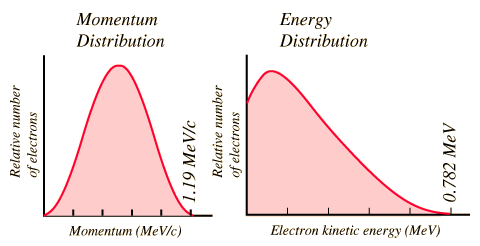
\includegraphics[scale=0.7]{nd}
  \caption{Electron properties in neutron decay in the rest frame. From \url{http://hyperphysics.phy-astr.gsu.edu/hbase/Particles/proton.html}}
  \label{fig:nd}
\end{figure}


\section{Backup}
\label{sec:backup}

Perturbation theory is developed more easily using the Hamiltonian formalism. We therefore consider a general field theory with a Hamiltonian
\begin{align}
  \label{eq:75}
  H=H_0+H_{\text{int}}\,
\end{align}
where $H_0$ is the free Hamiltonian and $H_{\text{int}}$ is the interaction term. The interaction term will be considered small. For instance in QED
\begin{align}
  H_{\text{int}}=\int d^3x\,\mathcal{H}_{\text{int}}=-\int d^3x\,\mathcal{L}_{\text{int}}
\end{align}
with
\begin{align}
  \mathcal{L}_{\text{int}}=-e A_\mu\overline{\psi}\gamma^\mu\psi
\end{align}
The smallnes of the interaction follows from the fact that the parameter which turns out to be relevatn for the perturbation expansion is $\alpha=e^2/4\pi\approx1/137$.


\begin{align}
  S S^\dagger=&(1+i T)(1-i T^\dagger)\nonumber\\
  &=1+i(T-T^\dagger)+T T^\dagger=1\,,\nonumber\\
\end{align}
\begin{align}
  T T^\dagger=-i(T-T^\dagger)\,.
\end{align}
Inserting a complete set of states we have
\begin{align}
  \langle b|T T^\dagger|a\rangle=&-i(\langle b|T|a\rangle-\langle b|T^\dagger|a\rangle)\nonumber\\
\langle b|T\left(\sum_n|n\rangle\langle n|\right)T^\dagger|a\rangle=&-i\left[\langle b|T|a\rangle-\left(\langle a|T|b\rangle\right)^\dagger\right]\nonumber\\
\sum_n\langle b|T|n\rangle\langle a|T|n\rangle^\dagger=&-i\left(\langle b|T|a\rangle-\langle a|T|b\rangle^*\right)\nonumber\\
\sum_n T_{bn}T_{an}^*=&-i\left(T_{ba}-T_{ab}^*\right)\,.\nonumber\\
\end{align}
if $a=b$
\begin{align}
  |T_{an}|^2=-i\operatorname{Im}T_{aa} \,.
\end{align}

%\left(\right)
%%% Local Variables: 
%%% mode: latex
%%% TeX-master: "beyond"
%%% End:
%instiki:category: QuantumFieldTheory
\chapter{Two body decays}
\label{cha:two-body-decays} %noinstiki
%instiki:
%instiki:***
%instiki:
%instiki:[[Beyond|Contents]]
%instiki:
%instiki:***
%instiki:
%instiki:* [Particle decays](#particle-decays)
%instiki:
%instiki:* [Width decay](#width-decay)
%instiki:
%instiki:* [Feynman Rules and trace theorems](#feynman-rules-trace)
%instiki:

In this chapter we use directly the Feynman rules for Fermions to carry out the calculation of the decay of the standard model Higgs into a pair of fermions. In chapter \ref{chap:fr} we will obtain the corresponding Feynman rules from the $S$--matrix expansion.




\section{Particle decays}
\label{sec:particle-decays}

Particle decay \cite{PD}  is the spontaneous process of one elementary particle transforming into other elementary particles. During this process, an elementary particle becomes a different particle with less mass and an intermediate particle such as $W$ boson in muon decay. 

For a particle of a mass $M$,  the differential decay width according Eq.~\eqref{eq:51}, is
\begin{equation}
  \label{eq:76}
 d\Gamma_n = \frac{(2\pi)^4}{2M}\left|\mathcal{M}\right|^2 d \Phi^{(n)} (P; p_1, p_2,\dots, p_n) \,
\end{equation}
The phase space can be determined from Eq.~\eqref{eq:50}
\begin{equation}
  d \Phi^{(n)} (P; p_1, p_2,\dots, p_n) = \delta^4 (P - \sum_{i=1}^n p_i) \left( \prod_{i=1}^n \frac{d^3 p_i}{(2\pi)^3 2 E_i} \right)\,.
\end{equation}
We will keep the $d\Gamma$ notation until all the integrals get evaluated. 

The two-body decays in eq.~\eqref{eq:152} is 
\begin{align}
\label{eq:154pd}
\frac{d\Gamma}{d\Omega}=
&\frac{1}{64 \pi^2M^3}\left|\mathcal{M}_{fi}\right|^2\lambda^{1/2}(M^2,m_2^2,m_1^2)
\end{align}



\section{Width decay}
\label{sec:width-decay}
%Poner las reglas de Feynman Aqui

Reglas de Feynman: Time direction from left to right.
\begin{itemize}
\item Initial particle: ${u}(p)$ 
\includegraphics{frip}
\item Initial antiparticle: $\bar{v}(p)$ 
\includegraphics{fria}
\item Final particle: $\bar{u}(p)$ 
\includegraphics{frfp}
\item Final antiparticle: ${v}(p)$ 
\includegraphics{frfa}

\end{itemize}

We consider now a general Yukawa interaction term
\begin{align}
  \mathcal{L}_{\text{int}}=hH\overline{f}_1 f_2
\end{align}
For the $H\to \overline{f}_1f_2$ decay.
The interaction between the Higgs boson with fermions\footnote{In this case we consider only electrons, by the formula is easy generalizable to other fermions} is given by the Yukawa interaction term \cite{lsm}
\begin{align}
\label{eq:155l}
\mathcal{L}_{\text{Higgs}}&=-G_{f}\frac{(v+H)}{\sqrt{2}}(\overline{f}_{R}f_{L}+\overline{f}_{L}f_{R})\nonumber\\
&=-\frac{G_{f}v}{\sqrt{2}}\overline{f}f-\frac{G_{f}H}{\sqrt{2}}\overline{f}f\nonumber\\
&=-m_f\overline{f}f-m_f\left(G_{F}\sqrt{2}\right)^{1/2}\overline{f}f
\end{align}
Such as the electro has acquired a mass $m_{e}=G_{f}\nu/\sqrt{2}$. On the other hand the coupling to be assigned to the process vertex is 
$G_{f}\sqrt{2}$ or $m_{f}/v=$. 

The decay process $H\to f\overline{f}$, is displayed in Fig. 
\ref{fig:a} %noinstiki

\begin{figure}[h!] %noinstiki
\begin{center} %noinstiki
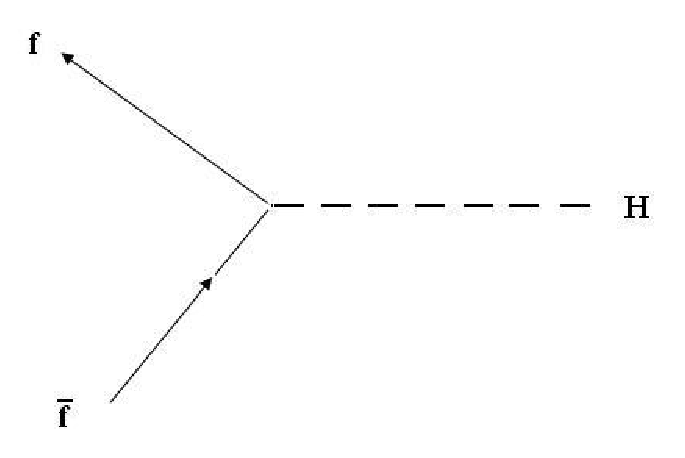
\includegraphics[scale=0.5]{decay}%noinstiki
\caption{Diagrama de proceso $H\to f\overline{f}$} %noinstiki
\label{fig:a} %noinstiki
\end{center} %noinstiki
\end{figure} %noinstiki

The Feynman rules, to be explained in Chapter~\ref{chap:fr} are indicated in Fig. 
\ref{fig:b}. %noinstiki

\begin{figure}[h] %noinstiki
\begin{center} %noinstiki
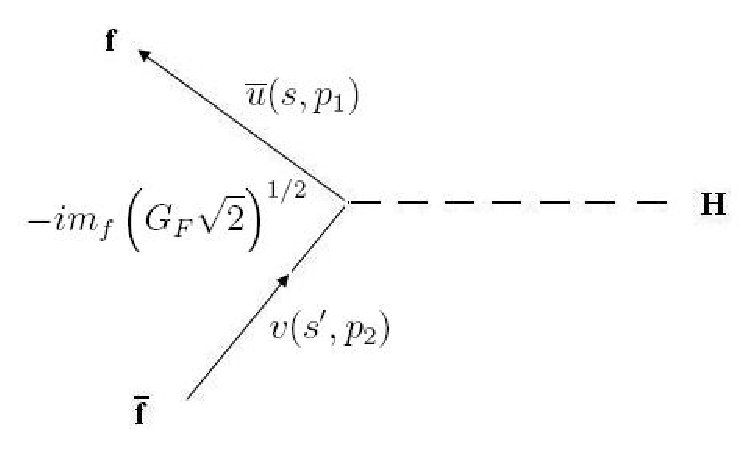
\includegraphics[scale=0.65]{feyn}%noinstiki
\caption{Reglas de Feynman del proceso $H\to f\overline{f}$}%noinstiki
\label{fig:b} %noinstiki
\end{center} %noinstiki
\end{figure} %noinstiki

In this way the scattering amplitude is 
\begin{equation}
i\mathcal{M}=-im_{f}\left(G_{F}\sqrt{2}\right)^{1/2}\overline{u}(s_1,
p_{1})v(s_2, p_{2}). 
\end{equation}
where $p_{1}$, $s$,  $p_{2}$ y $s_2$ are the momentum and spines of fermion and anti--fermion respectively.

For the general case
\begin{align}
i\mathcal{M}=-i h\overline{u}(s_1,p_{1})v(s_2, p_{2}). 
\end{align}
$h=m_{f}\left(G_{F}\sqrt{2}\right)^{1/2}$ in the standard models
Now, having into account that ${\gamma^{0}}^{\dag}=\gamma^{0}$
\begin{align*}
&(\overline{u}(s_1,p_{1})v(s_2, p_{2}))^{\dag}\\
&=v^{\dag}(s_2, p_{2})(\overline{u}(s_1,p_{1}))^{\dag}\\
&=v^{\dag}(s_2, p_{2})({u^{\dag}}(s_1,p_{1}){\gamma^{0}})^{\dag}\\
&=v^{\dag}(s_2, p_{2})({\gamma^{0}}^{\dag}u(s_1,p_{1}))\\
&=v^{\dag}(s_2, p_{2})(\gamma^{0}u(s_1,p_{1}))\\
&=\overline{v}(s_2,p_{2})u(s_1,p_{1}). 
\end{align*}
Squaring  $\mathcal{M}$,  and summing over possible polarization states of final particles, we have

\begin{equation}
\sum_{s_1,s_2}|\mathcal{M}|^{2}=h^2\sum_{s_1,s_2}(\overline{u}(s_1,p_{1})v(s_2,
p_{2}))(\overline{v}(s_2,p_{2})u(s_1,p_{1})). \label{eq:80}
\end{equation}
The several sums in Ec.~(\ref{eq:80}) can be calculated by expressing the products  $\overline{u}v$ y $\overline{v}u$ en in terms of their components, as follow
\begin{align}
\label{eq:81}
&\sum_{s_1,s_2}(\overline{u}(s_1,p_{1})v(s_2, p_{2}))(\overline{v}(s_2,p_{2})u(s_1,p_{1}))\nonumber\\
&=\sum_{s_1,s_2}(\overline{u}_{\alpha}(s_1,p_{1})v_{\alpha}(s_2, p_{2}))(\overline{v}_{\beta}(s_2,p_{2})u_{\beta}(s_1,p_{1}))\nonumber\\
&=\sum_{s_1,s_2}(u_{\beta}(s_1,p_{1})\overline{u}_{\alpha}(s_1,p_{1}))(v_{\alpha}(s_2, p_{2})\overline{v}_{\beta}(s_2,p_{2}))\nonumber\\
&=\sum_{s}u_{\beta}(s_1,p_{1})\overline{u}_{\alpha}(s_1,p_{1})\sum_{s_2}v_{\alpha}(s_2, p_{2})\overline{v}_{\beta}(s_2,p_{2})\nonumber\\
&=(\cancel{p}_{1}+m_{f})_{\beta\alpha}(\cancel{p}_{2}-m_{f})_{\alpha\beta}\nonumber\\
&=\operatorname{Tr}[(\cancel{p}_{1}+m_{f})(\cancel{p}_{2}-m_{f})]. 
\end{align}
Taking into account that  $\operatorname{Tr}[\gamma_{\nu}]=0$, and from the commutation relations for $\gamma_\mu$ matrices
\begin{align*}
\operatorname{Tr}[\gamma_{\mu}\gamma_{\nu}]&=\operatorname{Tr}[-\gamma_{\nu}\gamma_{\mu}+2g^{\mu\nu}]\\
&=\operatorname{Tr}[-\gamma_{\nu}\gamma_{\mu}]+2g^{\mu\nu}\operatorname{Tr}[\mathbf{1}]\\
&=\operatorname{Tr}[-\gamma_{\mu}\gamma_{\nu}]+2g^{\mu\nu}4 \qquad (\operatorname{Tr}[AB]=\operatorname{Tr}[BA])\\
\operatorname{Tr}[\gamma_{\mu}\gamma_{\nu}]&=4g^{\mu\nu}.
\end{align*}

In this way
\begin{align*}
&\operatorname{Tr}[(\cancel{p}_{1}+m_{1})(\cancel{p}_{2}-m_{2})]\\
&=\operatorname{Tr}[(\gamma_{\mu}p^{\mu}_{1}+m_{1})(\gamma_{\nu}p^{\nu}_{2}-m_{1})]\\
&=\operatorname{Tr}[\gamma_{\mu}\gamma_{\nu}p^{\mu}_{1}p^{\nu}_{2}-m_{2}\gamma_{\mu}p^{\mu}_{1}+m_{1}\gamma_{\nu}p^{\nu}_{2}-m_{1}m_2]\\
&=p^{\mu}_{1}p^{\nu}_{2}\operatorname{Tr}[\gamma_{\mu}\gamma_{\nu}]-4m_1 m_2\\
&=4g_{\mu\nu}p^{\mu}_{1}p^{\nu}_{2}-4m_1m_2\\
&=4(p_{1}\cdot p_{2}-m_1m_2). 
\end{align*}
where  $m_1$, $m_2$ are the final masses, and
\begin{equation*}
\sum_{s_1,s_2}|\mathcal{M}|^{2}=4h^2(p_{1}\cdot p_{2}-m_{1}m_2).
\end{equation*}
From eq.~\eqref{eq:153}
\begin{align}
  M=&E_1+E_2\nonumber\\
|\mathbf{p}_1|&=|\mathbf{p}_2|
\end{align}
Therefore
\begin{align}
  E_1E_2=\frac{M^2-E_1^2-E_2^2}{2}
\end{align}
\begin{align*}
p_{1}\cdot p_{2}-m^{2}_{f}&=E_{1}E_{2}-\mathbf{p}_{1}\cdot\mathbf{p}_{2}-m_1 m_2\\
&=E_{1}E_{2}+\mathbf{p}_{1}^2-m_1 m_2\\
&=\frac{M^2-E_1^2-E_2^2}{2}+\mathbf{p}_{1}^2-m_1 m_2\nonumber\\
&=\frac12\left(M^2-m_1^2-\mathbf{p}_1^2-m_2^2-\mathbf{p}_1^2\right)+\mathbf{p}_{1}^2-m_1 m_2\\
&=\frac12\left(M^2-m_1^2-m_2^2-2m_1m_2\right)\\
&=\frac12\left[M^2-(m_1-m_2)^2\right]
\end{align*}
%\left(\right)
Therefore, the scattering  amplitude is
\begin{equation}
\sum_{s_1,s_2}|\mathcal{M}|^{2}=2h^2\left[M^2-(m_1+m_2)^2\right]
\label{eq:82}
\end{equation}
Replacing back in eq.~\eqref{eq:154pd}
\begin{align}
\frac{d\Gamma}{d\Omega}=
&\frac{h^2}{32 \pi^2M^3}\lambda^{1/2}(M^2,m_2^2,m_1^2)\left[M^2-(m_1+m_2)^2\right]
\end{align}
After the integration $\int d\Omega_{\text{CM}}=4\pi$\footnote{$\int_0^{2\pi}d\phi\int_0^\pi\sin\theta d\theta=4\pi $} we have
\begin{align}
\Gamma=&\frac{h^2}{8 \pi M^3}\lambda^{1/2}(M^2,m_2^2,m_1^2)\left[M^2-(m_1+m_2)^2\right]
\end{align}
For $m_1=m_2=m_f$
\begin{align}
  \lambda^{1/2}(M^2,m_2^2,m_1^2)=&M^2\left(1-\frac{4m_f^2}{M^2}\right)^{1/2}\nonumber\\
\left[M^2-(m_1+m_2)^2\right]=&M^2\left(1-\frac{4m_f^2}{M^2}\right)
\end{align}
and therefore
\begin{align}
\Gamma(H\to f\overline{f})=&\frac{h^2}{8 \pi}M\left(1-\frac{4m_f^2}{M^2}\right)^{3/2}
\end{align}
In the case of the standard model Higgs with mass $M_H$ decaying to fermion pair, according to the Lagrangian in eq.~\eqref{eq:155l}

\begin{equation}
\Gamma(H\to f\overline{f})=\frac{M_{H}m_{f}^{2}G_{F}}{4\pi\sqrt{2}}
\left(1-4\frac{m^2_{f}}{M^2_{H}}\right)^{3/2}, 
\end{equation}

In the limit $m_{f}\ll M_{H}$ this expression reduces to 
\begin{equation}
\Gamma(H\to
f\overline{f})=\frac{M_{H}m_{f}^{2}G_{F}}{4\pi\sqrt{2}}. 
\end{equation}


\section{$e^+ e^- \to \mu^+\mu^-$}

\begin{align}
  \mathcal{L}=\frac{e^2}{s}
  \left[\bar v(k_2)\gamma^\lambda u(k_1)  \right]
  \left[\bar v(k_2)\gamma^\lambda u(k_1)  \right]
\end{align}

%%% Local Variables: 
%%% mode: latex
%%% TeX-master: "beyond"
%%% End:
%instiki:category: QuantumFieldTheory
\chapter{Feynman Rules}
\label{chap:fr} %noinstiki
%instiki:
%instiki:***
%instiki:
%instiki:[[Beyond|Contents]]
%instiki:
%instiki:***
%instiki:
%instiki:* [Interaction picture](#interaction-picture)
%instiki:
%instiki:* [Yukawa interaction](#feynman-diagrams)
%instiki:
%instiki:* [Scattering](#scattering)
%instiki:

When the case of interacting fields are considered, the particles can be created, destroyed and scattered. In essence this requires solving the coupled non-linear field equations for given conditions. This is an extremely difficult problem which has only been solved in perturbation theory.

In the Heisenberg picture, which we have so far been using, this program is still very complex, and it was decisive for the successful development of the theory to work instead in the interaction picture. In section \ref{sec:interaction-picture} we write the $S$--matrix expansion derived in Chapter~\ref{cha:s-matrix}, in the interaction picture. In section \ref{sec:feynman-diagrams} we show how to use the Wick expansion to calculate $S$--matrix elements involving scalars and spinors.

\section{Interaction picture}
\label{sec:interaction-picture}
This part is based in \cite{Mandl:1985bg}. 
In the Schr\"odinger Picture (SP) the time dependence is carried by the states according to the Scr\"odinger equation 
\begin{align}\
label{eq:84f}
  i\frac{\partial}{\partial t}|a,t\rangle_{\text{S}}=  i\frac{d}{dt}|a,t\rangle_{\text{S}}=  {H}|a,t\rangle_{\text{S}}
\end{align}
With the solution given in Eq.~\eqref{eq:39f}
\begin{align}
\label{eq:85f}
    |a,t\rangle_{\text{S}}=U(t,t_i)|a\rangle_{\text{S}}\,.
\end{align}
where $U$ is the unitary operator [see Eq.~\eqref{eq:40f}]
\begin{align}
 U\equiv U(t,t_i)= e^{-i H(t-t_i)}\,.
\end{align}
Given the state $|a,t\rangle_{\text{S}}$ in the SP, in the Heisenberg picture (HP) we defined the state
\begin{align}
\label{eq:86f}
  |a\rangle_H=U^\dagger|a,t\rangle_{\text{S}}=|a\rangle_{\text{S}}
\end{align}
Si $O^{\text{S}}$ in an operator in the SP, the corresponding Heisenberg operator is defined as
\begin{align}
\label{eq:87f}
  O^{\text{H}}(t)=U^\dagger O^{\text{S}}U
\end{align}
Hence, the transformation from HP to SP is unitary. At $t=t_i$, states and operators in the two pictures are the same. We see from Eq.~\eqref{eq:86f} that in the HP state vectors are constant in time, while from Eq.~\eqref{eq:87f} the Heisenberg operators evolve with time. Is convenient to keep the temporal label in the Heisenberg states
\begin{align}
  |a\rangle_H=|a,t_i\rangle_H
\end{align}
Eq.~\eqref{eq:87f} ensures the invariance of matrix elements and commutation relations:
\begin{align}
  {}_{\text{S}}\langle b,t|\,O^{\text{S}}\,|a,t\rangle_{\text{S}}=  {}_{\text{S}}\langle b,t|\,U O^{\text{H}}(t) U^\dagger\,|a,t\rangle_{\text{S}}=
{}_{\text{H}}\langle b,t_i|O^{\text{H}}(t)|a,t_i\rangle_{\text{H}}
\end{align}
\begin{align}
\left[O^{\text{S}},P^{\text{S}}\right]=c\Rightarrow\left[O^{\text{H}}(t),P^{\text{H}}(t)\right]=c
\end{align}
where $c$ is a constant.

Differentiation of Eq. \eqref{eq:87f} 
\begin{align}
  \frac{d}{dt}O^{\text{H}}(t)=&\left(\frac{d}{dt}U^\dagger\right)O^{\text{S}}U+
U^\dagger O^{\text{S}}\frac{d}{dt}U\nonumber\\
 =&i H\, U^\dagger O^{\text{S}}U+
U^\dagger O^{\text{S}}U(-i H)\nonumber\\
 =&-i ( O^{\text{H}}H-H O^{\text{H}})\,,
\end{align}
gives the Heisenberg equation of motion

\begin{align}
  i\frac{d}{dt}O^{\text{H}}(t)=\left[O^{\text{H}}(t),H\right]
\end{align}
The interaction picture (IP) arises if the Hamiltonian is split into two parts
\begin{align}
  H=H_0+H_{\text{I}}\,.
\end{align}
In quantum field theory $H_I$ will describe the interaction between two fields, themselves described by $H_0$

IP is related to the SP by the unitary transformation
\begin{align}
\label{eq:88f}
  U_i\equiv U_i(t,t_i)=e^{-i H_i(t-t_i)}\,,
\end{align}
in this way,
\begin{align}
\label{eq:89f}
  |a,t\rangle_{\text{I}}=U_0^\dagger|a,t\rangle_{\text{S}}\,,
\end{align}
and
\begin{align}
\label{eq:90f}
  O^{\text{I}}(t)=U^\dagger_0 O^{\text{S}}U_0\,.
\end{align}
Thus the relation between IP and SP is similar to that between HP and SP, but with the unitary transformation $U_0$ involving only the non--interacting Hamiltonian $H_0$. Note that both the vector states as the operators in the IP are time-dependent.

Differentiating Eq.~\eqref{eq:90f} gives the differential equation of motion operators in the IP:
\begin{align}
  i\frac{d}{dt}O^{\text{I}}(t)=\left[O^{\text{I}}(t),H_0\right]
\end{align}

Substituting Eq.~\eqref{eq:89f} into the Scr\"odinger Eq.~\eqref{eq:84f}, one obtains the equation of motion of state vectors in the IP, If the system is described by a time-dependent state vector $|\Phi(t)\rangle$
\begin{align}
  i\frac{d}{dt}|a,t\rangle_{\text{S}}=&  H^{\text{S}}|a,t\rangle_{\text{S}}\nonumber\\
  i\frac{d}{dt}\left(U_0|\Phi(t)\rangle\right)=&  H^{\text{S}}U_0|\Phi(t)\rangle\nonumber\\
  i\left(\frac{d}{dt}U_0\right)|\Phi(t)\rangle+iU_0\frac{d}{dt}|\Phi(t)\rangle=&  H^{\text{S}}U_0|\Phi(t)\rangle\nonumber\\
  U_0 H_0|\Phi(t)\rangle+iU_0\frac{d}{dt}|\Phi(t)\rangle=&  H^{\text{S}}U_0|\Phi(t)\rangle\nonumber\\
  U_0 H_0|\Phi(t)\rangle+iU_0\frac{d}{dt}|\Phi(t)\rangle=&  (H_0+H_I^{\text{S}})U_0|\Phi(t)\rangle\nonumber\\
  iU_0\frac{d}{dt}|\Phi(t)\rangle=&  H_I^{\text{S}}U_0|\Phi(t)\rangle\nonumber\\
  i\frac{d}{dt}|\Phi(t)\rangle=& U_0 H_I^{\text{S}}U_0|\Phi(t)\rangle
\end{align}
\begin{align}
\label{eq:91f}
  i\frac{d}{d t}|\Phi(t)\rangle_{\text{I}}=H^{\text{I}}_I\,|\Phi(t)\rangle_{\text{I}}\,,
\end{align}
where, as in Eq.~\eqref{eq:90f}
\begin{align}
  \label{eq:92f}
  H^{\text{I}}_I=e^{i H_0^{{\text{S}}}(t-t_i)}H^{\text{S}}_I e^{-i H_0^{{\text{S}}}(t-t_i)}
\end{align}
is the interaction Hamiltonian in the IP, with $H^{\text{S}}_I$ and $H^{\text{S}}_0$ being the interaction and free-field Hamiltonian in the SP. From now on we shall omit the labels I, used in the equations to distinguish the IP, as we shall be working exclusively in the IP in what follows.

Eq. \eqref{eq:91f} is a Scr\"odinger-like equation with the time dependent Hamiltonian $H_I(t)$. With the interaction switched off (i.e.  we put $H_I=0$), the state vector is constant in time. The interaction leads to the state $|\Phi(t)\rangle$ changing with time. Given that the system is in a state  $|i\rangle$ at an initial time $t=t_i$, i.e.
\begin{align}
\label{eq:93f}
  |\Phi(t_i)\rangle=|i\rangle\,,
\end{align}
the solution of Eq.~\eqref{eq:91f} with this initial condition gives the state $|\Phi(t)\rangle$ of the system at any other time $t$. It follows from the Hermicity of the operator $H_I(t)$ that the time development of the state $|\Phi(t)\rangle$ according to Eq.~\eqref{eq:91f} is a unitary transformation. Accordingly it preserves the normalization of states
\begin{align}
  \langle\Phi(t)|\Phi(t)\rangle=\text{const}.
\end{align}
and, more generally, the scalar product.

Clearly the formalism which we are here developing is not appropriate for the description of bound states but it is particularly suitable for scattering processes. In a collision processes the state vector $|i\rangle$ will define an initial state, long before the scattering occurs ($t_i=-\infty$), by specifying a definite number of particles, with definite properties and far apart from each other so that they do not interact. (For example $|i\rangle$ would specify a definite number of electrons, and positrons with given momenta and spins). In the scattering process, the particles will come close together, collide (i.e interact) and fly apart gain. Eq.~\eqref{eq:91f} determines the state $|\Phi(t)\rangle$ into which the initial state
\begin{align}
  |\Phi(-\infty)\rangle=|i\rangle\,,
\end{align}
evolves at $t=\infty$, long after the scattering is over and all particles are for apart again. The $S$--matrix relates $|\Phi(\infty)\rangle$ to $\Phi(-\infty)$ and is defined by
\begin{align}
  |\Phi(\infty)\rangle=S|\Phi(-\infty)\rangle=S|i\rangle\,,
\end{align}

A collision can lead to many different final states $|f\rangle$, and all these possibilities are constrained within $|\Phi(\infty)\rangle$.

The transition probability is given by
\begin{align}
  \left|\langle f|\Phi(\infty)\rangle\right|^2=  \left|\langle f|S|i\rangle\right|^2\equiv S_{f i}^2\,,
\end{align}
where $S_{f i}$ is the corresponding probability amplitude.

In order to calculate the $S$--matrix we must solve Eq.~\eqref{eq:91f} for the initial condition \eqref{eq:93f}. These equations can be combined into the integral equation
\begin{align}
 d |\Phi(t)\rangle=&-i d t\,H_I(t)|\Phi(t)\rangle\nonumber\\
\int_{|\Phi(-\infty)\rangle}^{|\Phi(t)\rangle} d |\Phi(t)\rangle=&-i \int_\infty^t d t_1\,H_I(t_1)|\Phi(t_1)\rangle\nonumber\\
|\Phi(t)\rangle-|\Phi(-\infty)\rangle=&-i \int_\infty^t d t_1\,H_I(t_1)|\Phi(t_1)\rangle\nonumber\\
\end{align}

\begin{align}
\label{eq:94f}
  |\Phi(t)\rangle=|i\rangle-i\int_{-\infty}^t d t_1\,H_I(t_1)|\Phi(t_1)\rangle\,.
\end{align}
In the limit $t\to\infty$
\begin{align}
  |\Phi(\infty)\rangle=S^{(0)}|i\rangle-i\int_{-\infty}^\infty d t_1\,H_I(t_1)|\Phi(t_1)\rangle\,.
\end{align}
where 
\begin{align}
  S^{(0)}=1\,.
\end{align}
From Eq.~\eqref{eq:94f} we can obtain $|\Phi(t_1)\rangle$ at next order:
\begin{align}
  |\Phi(t_1)\rangle=&|i\rangle-i\int_{-\infty}^{t_1} d t_2\,H_I(t_2)|\Phi(t_2)\rangle\,.
\end{align}


This equation then can  be solved iteratively. If $H_I$ is small we can solve this equation by iteration
\begin{align}
\label{eq:95f}
  |\Phi(t)\rangle=|i\rangle+(-i)\int_{-\infty}^t d t_1 H_I(t_1)|i\rangle+(-i)^2\int_{-\infty}^t d t_1\int_{-\infty}^{t_1} d t_2\,H_I(t_1)H_I(t_2)|\Phi(t_2)\rangle\,.
\end{align}
In the limit $t\to\infty$
\begin{align}
  |\Phi(t)\rangle=&\left[S^{(0)}+(-i)\int_{-\infty}^\infty d t_1 H_I(t_1)\right]|i\rangle+(-i)^2\int_{-\infty}^\infty d t_1\int_{-\infty}^{t_1} d t_2\,H_I(t_1)H_I(t_2)|\Phi(t_2)\rangle\nonumber\\
  =&\left(S^{(0)}+S^{(1)}\right)|i\rangle+(-i)^2\int_{-\infty}^\infty d t_1\int_{-\infty}^{t_1} d t_2\,H_I(t_1)H_I(t_2)|\Phi(t_2)\rangle\,,
\end{align}
where 
\begin{align}
  S^{(1)}=(-i)\int_{-\infty}^\infty d t_1 H_I(t_1)\,.
\end{align}
The next order of Eq.~\eqref{eq:95f} is
\begin{align}
  |\Phi(t)\rangle=&|i\rangle+(-i)\int_{-\infty}^t d t_1 H_I(t_1)|i\rangle+(-i)^2\int_{-\infty}^t d t_1\int_{-\infty}^{t_1} d t_2\,H_I(t_1)H_I(t_2)\nonumber\\
  &\times\left[|i\rangle+(-i)\int_{-\infty}^{t_2} d t_3 H_I(t_3)|i\rangle+(-i)^2\int_{-\infty}^{t_2} d t_3\int_{-\infty}^{t_3} d t_4\,H_I(t_3)H_I(t_4)|\Phi(t_4)\rangle\right]
\end{align}
\begin{align}
  |\Phi(t)\rangle=&|i\rangle+(-i)\int_{-\infty}^t d t_1 H_1(t_1)|i\rangle+(-i)^2\int_{-\infty}^t d t_1\int_{-\infty}^{t_1} d t_2\,H_I(t_1)H_I(t_2)|i\rangle\nonumber\\
  &+(-i)^3\int_{-\infty}^t d t_1\int_{-\infty}^{t_1} d t_2\int_{-\infty}^{t_2} d t_3\,H_I(t_1)H_I(t_2) H_1(t_3)|i\rangle\nonumber\\
  &+(-i)^4\int_{-\infty}^t d t_1\int_{-\infty}^{t_1}d t_2 \int_{-\infty}^{t_2} d t_3\int_{-\infty}^{t_3}d t_4 \,H_I(t_1)H_I(t_2)\,H_I(t_3)H_I(t_4)|\Phi(t_4)\rangle
\end{align}
In the limit $t\to\infty$
\begin{align}
  |\Phi(t)\rangle=&\left(S^{(0)}+S^{(1)}+S^{(2)}+S^{(3)}\right)|i\rangle\nonumber\\
  &+(-i)^4\int_{-\infty}^\infty d t_1\int_{-\infty}^{t_1}d t_2 \int_{-\infty}^{t_2} d t_3\int_{-\infty}^{t_3}d t_4 \,H_I(t_1)H_I(t_2)\,H_I(t_3)H_I(t_4)|\Phi(t_4)\rangle
\end{align}
where
\begin{align}
  S^{(2)}=&(-i)^2\int_{-\infty}^\infty d t_1\int_{-\infty}^{t_1} d t_2\,H_I(t_1)H_I(t_2)\nonumber\\
  S^{(3)}=&(-i)^3\int_{-\infty}^\infty d t_1\int_{-\infty}^{t_1} d t_2\int_{-\infty}^{t_2} d t_3\,H_I(t_1)H_I(t_2) H_1(t_3)
\end{align}

and so on we obtain the $S$--matrix
\begin{align}
  S=&\sum_{n=0}^\infty S^{(n)}\nonumber\\
  =&1+\sum_{n=1}^\infty\frac{(-i)^n}{n!}\int_{-\infty}^{\infty}d t_1\,\int_{-\infty}^{t_1} d t_2\ldots\int_{-\infty}^{t_{n-1}}d t_n\,{H}_I(t_1){H}_I(t_2)\ldots{H}_I(t_n)\,.
\end{align}


\section{Atomic decay}
\label{sec:atomic-decay}

Here we follow closelly \cite{Gross:1993} chapter 3.

For the atomic decay at first order in perturbation theory, we have
\begin{align}
  S_{\beta\alpha}^{(1)}=-i \int_{-\infty}^\infty dt\, \left\langle\beta\left|H_I(t)\right|\alpha\right\rangle.
\end{align}
where the Hamiltonian in the interaction picture is
\begin{align}
  H=&H_A+H_{EM}+H_I(t)=H_0+H_I(t)\,,
\end{align}
where, following the definition of the interaction picture
\begin{align}
  \psi_a(r,t)=&e^{-i H_A t}\psi_a(r)\nonumber\\
=&U_A(t)\psi_a(r)\,,
\end{align}

\begin{align}
  H_I(t)=U_A^{-1}H'_I(t)U_A\,.
\end{align}
The several terms of the Hamiltonia are

\begin{align}
  H_A=\frac{\mathbf{p}_e^2}{2m}-\frac{Z\alpha}{r_e}\,,
\end{align}
\begin{align}
  H_{EM}=\frac{1}{2}\int d^3r\left\{:\boldsymbol{\pi}^2(r,t):+:\mathbf{B}^2(r,t):\right\}\,,
\end{align}
\begin{align}
  H_I'(t)=\left\{\frac{e}{2m}\left(\mathbf{p}_e\cdot\mathbf{A}(r_e,t)+\mathbf{A}(r_e,t)\cdot \mathbf{p}_e
+\frac{e^2}{2m}\mathbf{A}^2(r_e,t)\right)\right\}\,,
\end{align}
and $\alpha=e^2/(4\pi)$.
The states as defined as
\begin{align}
  |a,n\rangle=\psi_a(r_e)|n\rangle\,.
\end{align}
The scalar product of the atomic states requires an integration over the coordinate $r_e$
\begin{align}
  \label{eq:163f}
   \langle a',n'|a,n\rangle=\int d^3r\,\psi_{a'}^*(r_e)\psi_a(r_e)\langle n'|n\rangle.
\end{align}

For one photon decay of an initial atomic state $a$ into a final atomic state $b$ and a photon of energy $\omega_n$ and polarization $\lambda$, the states are
\begin{align}
  |\alpha\rangle=&|\alpha,0\rangle=\psi_a(r_e)|0\rangle\nonumber\\
  |\beta\rangle=&|b,1_{n\lambda}\rangle=\psi_b(r_e)|1_{n\lambda}\rangle\,,
\end{align}
where
\begin{align}
  |1_{n\lambda}\rangle=a_{n\lambda}^\dagger|0\rangle
\end{align}
is the one-photon state with frequency $\omega_n$ and polarization $\lambda$. Since
\begin{align}
 \langle1_{n\lambda}|\mathbf{A}^2|0\rangle\supset\langle1_{n\lambda}|(a_{n\lambda}^\dagger a_{n\lambda}^\dagger+a_{n\lambda}^\dagger a_{n\lambda}+a_{n\lambda}a_{n\lambda})|0\rangle=\langle0|1_{n\lambda}\rangle=0
\end{align}
and
\begin{align}
\left(\mathbf{p}_e\cdot\mathbf{A}(r_e,t)+\mathbf{A}(r_e,t)\cdot \mathbf{p}_e\right)\psi_a(r_e)=&
-i\left(\boldsymbol{\nabla}_e\cdot\mathbf{A}(r_e,t)+\mathbf{A}(r_e,t)\cdot\boldsymbol{\nabla}_e\right)\psi_a(r_e)
\nonumber\\
=&-i\left\{\left(\boldsymbol{\nabla}_e\cdot\mathbf{A}\right)\psi_a
+\mathbf{A}\cdot\boldsymbol{\nabla}_e\psi_a
+\mathbf{A}\cdot\boldsymbol{\nabla}_e\psi_a\right\}\nonumber\\
=&-i\left\{2\mathbf{A}\cdot\boldsymbol{\nabla}_e\psi_a\right\}\,,
\end{align}
where $\boldsymbol{\nabla}\cdot\mathbf{A}=0$ was used.

With all of this we have a simplified formula
\begin{align}
\label{eq:164f}
  S_{ba}=&-i\int_{-\infty}^\infty dt\langle b,1_{n\lambda}|U_A^{-1}\left(-\frac{ie}{m}\mathbf{A}(r_e,t)\cdot\boldsymbol{\nabla}_e\right)
  U_A|a,0\rangle\nonumber\\
  S_{ba}=&-i\int_{-\infty}^\infty dt\langle b,1_{n\lambda}|U_A^{-1}\left(-\frac{ie}{m}\mathbf{A}(r_e,t)\cdot\boldsymbol{\nabla}_e\right)
  U_A|a,0\rangle\nonumber\\
  S_{ba}=&-i\int_{-\infty}^\infty dt\langle b,1_{n\lambda}|e^{iE_b t}\left(-\frac{ie}{m}\mathbf{A}(r_e,t)\cdot\boldsymbol{\nabla}_e\right)
  e^{-i E_a t}|a,0\rangle\nonumber\\
  =&-\int_{-\infty}^\infty dt\,e^{i(E_b-E_a)t}\int d^3r_e\langle1_{n\lambda}|\psi_b^*(r_e)\frac{e}{m}\left(\mathbf{A}(r_e,t)\cdot\boldsymbol{\nabla}_e\right)
  \psi_a(r)|0\rangle\nonumber\\
 =&-\int_{-\infty}^\infty dt\,e^{i(E_b-E_a)t}\frac{e}{m}\int d^3r_e\left\{\psi_b^*(r_e)\boldsymbol{\nabla}_e\psi_a(r)\right\}\cdot 
  \langle1_{n\lambda}|\mathbf{A}(r_e,t)|0\rangle.
\end{align}
Since
\begin{align}
  \langle1_{n\lambda}|\mathbf{A}(r_e,t)|0\rangle=&\sum_{n'\lambda'}\frac{1}{\sqrt{2\omega_{n'}L^3}}\boldsymbol{\epsilon}^{\lambda'}_{n'}
  \langle1_{n\lambda}|a^\dagger_{n'\lambda'}|0\rangle e^{i k_{n'}\cdot x_e}\nonumber\\
=&\sum_{n'\lambda'}\frac{1}{\sqrt{2\omega_{n'}L^3}}\boldsymbol{\epsilon}^{\lambda'}_{n'}
  \langle1_{n\lambda}|a^\dagger_{n'\lambda'}|0\rangle e^{i k_{n}\cdot x_e}\nonumber\\
=&\frac{1}{\sqrt{2\omega_{n}L^3}}\boldsymbol{\epsilon}^{\lambda}_{n}
  \langle1_{n\lambda}|1_{n\lambda}\rangle e^{i k_{n'}\cdot x_e}\nonumber\\
=&\frac{1}{\sqrt{2\omega_{n}L^3}}\boldsymbol{\epsilon}^{\lambda}_{n}
  e^{i \omega_n t-\mathbf{k}_n\cdot\mathbf{r}_e}\,.
\end{align}
Inserting this expression into (\ref{eq:164f}) gives
%%% faltan detalles
\begin{align}
  S_{ba}=-i2\pi \delta(E_b+\omega_n-E_a)\frac{1}{\sqrt{L^3}}M_{ba}\,, 
\end{align}
where the decaya amplitude $M_{ba}$ is
\begin{align}
  M_{ba}=-i\frac{e}{m}\frac{1}{2\omega_n}\int d^3r_e\,e^{-i\mathbf{k}_n\cdot\mathbf{r}_e}
  \psi_b^*(r_e)\boldsymbol{\epsilon}^{\lambda}_{n}\cdot\boldsymbol{\nabla}_e\psi_a(r)\,.
\end{align}
In most atomic decays, the energy of the emmited photon, which is equal to $\omega_n=E_b-E_a$, is much less than $1/R$, where $R$ is the
size of the atomic system, and hence the maximum range of the integral over $r_e$. In this case, the dipole approximation 
\begin{align}
  e^{-i\mathbf{k}_n\cdot\mathbf{r}_e}\approx1
\end{align}
is extremely good. Then we have
\begin{align}
  M_{ba}=\frac{e}{m}\frac{1}{\sqrt{2\omega_n}}\boldsymbol{\epsilon}^{\lambda}_{n}\cdot\mathbf{p}_{ba}\,,
\end{align}
where
\begin{align}
  \mathbf{p}_{ba}=-i\int d^3r_e \psi_b^*(r_e)\boldsymbol{\nabla}_e\psi_a(r_e).
\end{align}
The diferential decay rate, and using
\begin{align}
  [2\pi \delta(E_f-E_i)]^2=2\pi \delta(E_f-E_i) T \,,
\end{align}
we have
\begin{align}
  \Delta W_{ba}=&\lim_{T\to \infty}\frac{|S_{ba}(T/2,-T/2)|^2}{T}\nonumber\\
  =&\lim_{T\to \infty}\frac{1}{T}2\pi \delta(E_b+\omega_n-E_a) T \frac{1}{L^3}|M_{ba}|^2\nonumber\\
  =&2\pi\delta(E_b+\omega_n-E_a)\frac{1}{L^3}|M_{ba}|^2
\end{align}
Then
\begin{align}
  \Delta W_{ba}=&\frac{2\pi}{V}\delta(E_b+\omega_n-E_a)\frac{e^2}{2\omega_n m^2}|\boldsymbol{\epsilon}^{\lambda}_{n}\cdot\mathbf{p}_{ba}|^2\,.
\end{align}
Summing over all final photon states to get the total $a\to b$ decay rate gives
\begin{align}
  W_{ba}=&\sum_{n,\lambda}\frac{2\pi}{V}\delta(E_b+\omega_n-E_a)\frac{e^2}{2\omega_n m^2}|\boldsymbol{\epsilon}^{\lambda}_{n}\cdot\mathbf{p}_{ba}|^2\nonumber\\
  =&\sum_{\lambda}\sum_n\frac{2\pi}{V}\delta(E_b+\omega_n-E_a)\frac{e^2}{2\omega_n m^2}|\boldsymbol{\epsilon}^{\lambda}_{n}\cdot\mathbf{p}_{ba}|^2\,.
\end{align}
Using
\begin{align}
  \sum_n\to \frac{V}{(2\pi)^3}\int d^3k
\end{align}
\begin{align}
   W_{ba}=&\sum_{\lambda}\int\frac{d^3k}{(2\pi)^2}\delta(E_b+\omega_n-E_a)\frac{e^2}{2\omega m^2}|\boldsymbol{\epsilon}^{\lambda}_{n}\cdot\mathbf{p}_{ba}|^2\nonumber\\
=&\frac{e^2}{2m^2}\sum_{\lambda}\int\frac{d^3k}{(2\pi)^2\omega}\delta(E_b+\omega_n-E_a)|\boldsymbol{\epsilon}^{\lambda}_{n}\cdot\mathbf{p}_{ba}|^2\nonumber\\
=&\frac{e^2}{2m^2}\sum_{\lambda}\int|\mathbf{k}|^2d|\mathbf{k}|\int d\Omega\frac{d^3k}{(2\pi)^2\omega}\delta(E_b+\omega-E_a)|\boldsymbol{\epsilon}^{\lambda}_{n}\cdot\mathbf{p}_{ba}|^2\,.
\end{align}
By using $|\mathbf{k}|=\omega$, we have
\begin{align}
  W_{ba}=&\frac{e^2}{2m^2}\sum_{\lambda}\int d\omega\frac{\omega}{(2\pi)^2}\delta(E_b+\omega-E_a)\int d\Omega|\boldsymbol{\epsilon}^{\lambda}_{n}\cdot\mathbf{p}_{ba}|^2\nonumber\\
=&\frac{e^2}{4\pi}\left(\frac{\omega}{2\pi m^2}\right)\sum_{\lambda}\int d\Omega|\boldsymbol{\epsilon}^{\lambda}_{n}\cdot\mathbf{p}_{ba}|^2\,,
\end{align}
where $\omega=E_b-E_a$.
%%Faltan detalles
Integrating over all directions $\widehat{\mathbf{k}}$ of the outgoing photon
\begin{align}
  \sum_{\lambda}\int d\Omega|\boldsymbol{\epsilon}^{\lambda}_{n}\cdot\mathbf{p}_{ba}|^2=\frac{8\pi}{3}|\mathbf{p}_{ba}|^2\,.
\end{align}
Then the total rate for the decay of the state $a$ into $b$ is
\begin{align}
  W_{ba}=\frac{e^2}{4\pi}\left(\frac{4\omega}{3 m^2}\right)|\mathbf{p}_{ba}|^2\,.
\end{align}

%\left(\right)


\section{Yukawa interaction}
\label{sec:feynman-diagrams}
As a concrete example, we take a theory with a fermion field and scalar field, which interact via the Yukawa interaction \cite{Lahiri:2005sm}:
\begin{align}
  \mathcal{L}_{\text{int}}=-h \overline{\psi}\psi\phi\,.
\end{align}
Let the quantum of the field $\phi$ be denoted by $B$, since the particle is a boson. The quanta of the fermionic field $\psi$ will be called electrons. The mass of $B$ is $M$, and the mass of the electron by $m$. Suppose $M\gt 2m$,  so that kinematically it is possible to have the $B$ particle decay into an electron-positron pair. The process is denoted by
\begin{align}
  B(k)\to e^-(p)+e^+(p')\,,
\end{align}
where $k$, $p$, $p'$ are the 4--momenta of the particles.

For the interaction Hamiltonian we have
\begin{align}
  \mathcal{H}_I=h:\overline{\psi}\psi\phi:
\end{align}
where the required ordered product will be explained in next section.
The term linear in the interaction Hamiltonian in the $S$--matrix.  It is
\begin{align}
  S^{(1)}=\nonumber\\
=&-i h \int d^4x:\overline{\psi}\psi\phi:\,.
\end{align}

\begin{align}
  S^{(1)}=-i h \int d^4x:(\overline{\psi}_++\overline{\psi}_-)(\psi_++\psi_-)(\phi_++\phi_-):\,.
\end{align}




\begin{align}
 \mathcal{L}_{int}=&-h:\left( \bar{\psi}_{+}+\bar{\psi}_{-}\right) \left( \psi_{+}+\psi_{-}\right) \left( \phi_{+}+\phi_{-}\right):\nonumber\\
=&:
\bar{\psi}_{+}\psi_{+}\phi_{+}+ 
\bar{\psi}_{+}\psi_{+}\phi_{-}+ 
\bar{\psi}_{+}\psi_{-}\phi_{+}+ 
\bar{\psi}_{+}\psi_{-}\phi_{-}+ 
\bar{\psi}_{-}\psi_{+}\phi_{+}\nonumber\\ 
&+\bar{\psi}_{-}\psi_{+}\phi_{-}+ 
\bar{\psi}_{-}\psi_{-}\phi_{+}+ 
\bar{\psi}_{-}\psi_{-}\phi_{-} 
:\nonumber\\
=&\bar{\psi}_{-}\psi_{-}\phi_{+}+ 
\end{align}


To check that only the ordered terms are different from zero we can analyse the full terms for initial and final states defined as $|i\rangle=|0_{\bar{\psi}},0_{\psi},1_{\phi}\rangle$ y $\langle f|=\langle 1_{\bar{\psi}},1_{\psi},0_\phi|$. 

\begin{align}
 \phi_{+} | n_{\phi} \rangle  \propto& |n-1_{\phi}\rangle & \langle n_{\phi}|\phi_{+} \propto& \langle n+1_{\phi}|
\end{align}

y

\begin{align}
 \phi_{-} |n_{\phi}\rangle  \propto& |n+1_{\phi}\rangle&  \langle n_{\phi}| \phi_{-} \propto& \langle n-1_{\phi}|
\end{align}

Y lo mismo tendremos bien sea para un campo fot\'onico o fermi\'onico.

El Langrangiano de interacci\'on de nuestro inter\'es est\'a dado por

\begin{equation}
 \mathcal{L}_{int}=-h\bar{\psi}\psi\phi
\end{equation}

Que en t\'erminos de las componentes $+$ y $-$ de los campos se puede expresar como


De desarrollo del langrangiano en las componentes de los campos, vemaos qu\'e t\'erminos contribuyen al elemento de matriz

\begin{align*}
 \langle1_{\bar{\psi}},1_{\psi},0_{\phi}|\bar{\psi}_{+}\psi_{+}\phi_{+}|0_{\bar{\psi}},0_{\psi},1_{\phi}\rangle  &\propto  \langle2_{\bar{\psi}},2_{\psi},0_{\phi}|0_{\bar{\psi}},0_{\psi},0_{\phi}\rangle =0\\ 
 \langle1_{\bar{\psi}},1_{\psi},0_{\phi}|\bar{\psi}_{+}\psi_{+}\phi_{-}|0_{\bar{\psi}},0_{\psi},1_{\phi}\rangle  &\propto  \langle2_{\bar{\psi}},2_{\psi},0_{\phi}|0_{\bar{\psi}},0_{\psi},2_{\phi}\rangle =0\\ 
 \langle1_{\bar{\psi}},1_{\psi},0_{\phi}|\bar{\psi}_{+}\psi_{-}\phi_{+}|0_{\bar{\psi}},0_{\psi},1_{\phi}\rangle  &\propto  \langle2_{\bar{\psi}},0_{\psi},0_{\phi}|0_{\bar{\psi}},0_{\psi},0_{\phi}\rangle =0\\ 
 \langle1_{\bar{\psi}},1_{\psi},0_{\phi}|\bar{\psi}_{+}\psi_{-}\phi_{-}|0_{\bar{\psi}},0_{\psi},1_{\phi}\rangle  &\propto  \langle2_{\bar{\psi}},0_{\psi},0_{\phi}|0_{\bar{\psi}},0_{\psi},2_{\phi}\rangle =0\\ 
 \langle1_{\bar{\psi}},1_{\psi},0_{\phi}|\bar{\psi}_{-}\psi_{+}\phi_{+}|0_{\bar{\psi}},0_{\psi},1_{\phi}\rangle  &\propto  \langle0_{\bar{\psi}},2_{\psi},0_{\phi}|0_{\bar{\psi}},0_{\psi},0_{\phi}\rangle =0\\ 
 \langle1_{\bar{\psi}},1_{\psi},0_{\phi}|\bar{\psi}_{-}\psi_{+}\phi_{-}|0_{\bar{\psi}},0_{\psi},1_{\phi}\rangle  &\propto  \langle0_{\bar{\psi}},2_{\psi},0_{\phi}|0_{\bar{\psi}},0_{\psi},2_{\phi}\rangle =0\\ 
 \langle1_{\bar{\psi}},1_{\psi},0_{\phi}|\bar{\psi}_{-}\psi_{-}\phi_{+}|0_{\bar{\psi}},0_{\psi},1_{\phi}\rangle  &\propto  \langle0_{\bar{\psi}},0_{\psi},0_{\phi}|0_{\bar{\psi}},0_{\psi},0_{\phi}\rangle \neq 0\\
 \langle1_{\bar{\psi}},1_{\psi},0_{\phi}|\bar{\psi}_{-}\psi_{-}\phi_{-}|0_{\bar{\psi}},0_{\psi},1_{\phi}\rangle  &\propto  \langle0_{\bar{\psi}},0_{\psi},0_{\phi}|0_{\bar{\psi}},0_{\psi},2_{\phi}\rangle =0
\end{align*}


The only term that contributes to the matrix element of the process is
\begin{align}
  \label{eq:97f}
  -i h \int d^4x\overline{\psi}_-\psi_-\phi_+\,.
\end{align}

\begin{figure} %noinstiki
  \centering %noinstiki
  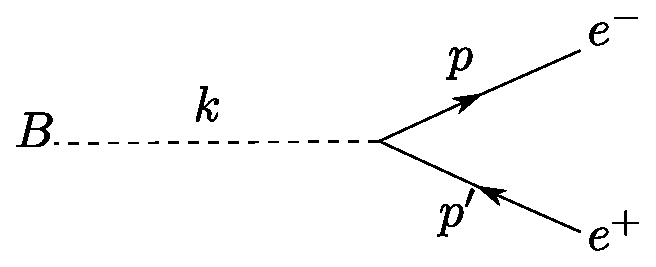
\includegraphics[scale=0.6]{Btoee} %noinstiki
  \caption{Feynman diagrams for $B\to e^+ e^-$} %noinstiki
  \label{fig:btoee} %noinstiki
\end{figure} %noinstiki
Let us define the one--particle states as in eq.~\eqref{eq:38f}

\begin{align}
  | B(\mathbf{p})\rangle\equiv\sqrt{\frac{1}{V}}a^\dagger_{\mathbf{p}}|0\rangle 
\end{align}
From eq.~\eqref{eq:79f} 
\begin{align}
  \label{eq:77f}
   | e^-(\mathbf{p},s)\rangle\equiv&\sqrt{\frac{1}{V}}a^\dagger_s(\mathbf{p})|0\rangle\nonumber\\
   | e^+(\mathbf{p},s)\rangle\equiv&\sqrt{\frac{1}{V}}{b}^\dagger_s(\mathbf{p})|0\rangle\,, 
\end{align}
Using the commutation relations, our states are then normalized as
\begin{align}
\langle B(\mathbf{p})| B(\mathbf{p}')\rangle=&\frac{(2\pi)^3}{V}\delta^3(\mathbf{p}-\mathbf{p}')\nonumber\\
\langle e^-(\mathbf{p},s)| e^-(\mathbf{p}',s')\rangle=&\frac{(2\pi)^3}{V}\delta_{s s'}\delta^3(\mathbf{p}-\mathbf{p}')\nonumber\\
\langle e^+(\mathbf{p},s)| e^+(\mathbf{p}',s')\rangle=&\frac{(2\pi)^3}{V}\delta_{s s'}\delta^3(\mathbf{p}-\mathbf{p}')
\end{align}
As established in Sec.~\ref{sec:fock-space-real}, it is convenient to work in the discrete limit where \eqref{eq:26f}
\begin{align}
   \delta^3(\mathbf{0})=\frac{V}{(2\pi)^3}\,.
\end{align}

Now we can write down the action of various field operators on different one particles states. 
Using the Fourier decomposition  of the scalar field in eq.~\eqref{eq:37f}, and taking into account that 
$a_{\mathbf{p}}|0\rangle=0$, we have
\begin{align}
\label{eq:98f}
   \phi_+(x)|B(\mathbf{k})\rangle=&\int d^3p \frac{1}{(2\pi)^3\sqrt{2\omega_{p} }}
\widehat{a}_{p} e^{-i p\cdot x }
|B(\mathbf{k})\rangle\nonumber\\
=&\int d^3p \frac{1}{(2\pi)^3\sqrt{2\omega_{p}}}
\widehat{a}_\mathbf{p} e^{-i p\cdot x }
\frac{1}{\sqrt{V}}\, \widehat{a}^\dagger_{\mathbf{k}}|0\rangle\nonumber\\
  =&\int d^3p \frac{1}{(2\pi)^3\sqrt{2\omega_{p}V}} e^{-i p\cdot x }
\, [\widehat{a}_{\mathbf{p}},\widehat{a}^\dagger_{\mathbf{k}}]|0\rangle\,.
\end{align}
%check normalization!
By usinbg the commutation relations in eq.~\eqref{eq:32f} we have

\begin{align}
\phi_+(x)|B(\mathbf{k})\rangle  
=&\int d^3p \frac{\delta^{(3)}(\mathbf{p}-\mathbf{k})}{\sqrt{2\omega_{p}V}}
 e^{-i p\cdot x }|0\rangle
\end{align}
\begin{align}
\phi_+(x)|B(\mathbf{k})\rangle  
=&\frac{1}{\sqrt{2\omega_{k}V}}e^{-i k\cdot x }|0\rangle
\end{align}
Similarly, we have


\begin{align}
  \label{eq:99f}
  \phi_+(x)|B(\mathbf{k})\rangle=&\frac{1}{\sqrt{2 \omega_k V}}e^{-i k\cdot x}|0\rangle\nonumber\\
  \psi_+(x)|e^-(\mathbf{p},s)\rangle=&\frac{1}{\sqrt{2 E_p V}}u_s(\mathbf{p})e^{-i p\cdot x}|0\rangle\nonumber\\
  \overline{\psi}_+(x)|e^+(\mathbf{p}',s')\rangle=&\frac{1}{\sqrt{2 E_{p'} V}}\bar{v}_{s'}(\mathbf{p}')e^{-i p'\cdot x}|0\rangle\,,
\end{align}

where $\omega_k$ and $E_p$ represent the energies of the scalar and the electron for the 3-momenta in the subscripts.

Similarly, for the adjoint operators
\begin{align}
  \label{eq:100f}
   \langle B(\mathbf{k})|\phi_-(x)=&\langle0|\frac{1}{\sqrt{2 \omega_k V}}e^{i k\cdot x}\nonumber\\
  \langle e^-(\mathbf{p},s)|\overline{\psi}_-(x)=&\langle0|\frac{1}{\sqrt{2 E_p V}}\bar{u}_s(\mathbf{p})e^{i p\cdot x}\nonumber\\
  \langle e^+(\mathbf{p}',s')|\psi_-(x)=&\langle0|\frac{1}{\sqrt{2 E_{p'} V}}v_{s'}(\mathbf{p}')e^{i p'\cdot x}\,,
\end{align}
In the lowest order the only term which contributes to the matrix element is the term shown in Eq.~\eqref{eq:97f}
The matrix element at first order in Eq.~\eqref{eq:96f}, between the initial and the final state is then
\begin{align}
  S_{fi}^{(1)}=-i h \int d^4x\left\langle e^-(p)e^+(p')\left|\overline{\psi}_-\psi_-\phi_+\right|B(k)\right\rangle\,.
\end{align}
Using Eqs.~\eqref{eq:99f}\eqref{eq:100f}, we obtain
\begin{align}
  S_{fi}^{(1)}=&(-i h)\bar{u}_s(\mathbf{p}) v_{s'}(\mathbf{p}')
\int d^4x\,e^{i(p+p'-k)\cdot x}\frac{1}{\sqrt{2\omega_k V}}\frac{1}{\sqrt{2E_p V}}\frac{1}{\sqrt{2E_{p'} V}}\,.
\end{align}
Since
\begin{align}
  \int d^4x\,e^{i(p+p'-k)\cdot x}=(2\pi)^4\delta^4(k-p-p')\,,
\end{align}
we obtain
\begin{align}
  S_{fi}^{(1)}=&\left[\frac{1}{\sqrt{2\omega_k V}}\frac{1}{\sqrt{2E_p V}}\frac{1}{\sqrt{2E_{p'} V}}\right]
(2\pi)^4\delta^4(k-p-p')\left[(-i h)\bar{u}_s(\mathbf{p}) v_{s'}(\mathbf{p}')\right]
\end{align}
Comparing with Eq.~\eqref{eq:46f} we have therefore that the relativistic matrix element is
\begin{align}
  i\mathcal{M}_{fi}=(-i h)\bar{u}_s(\mathbf{p}) v_{s'}(\mathbf{p}')\,,
\end{align}
and everything else is the history presented in Chapter~\ref{cha:two-body-decays}. 

\section{Wick Theorem}
\label{sec:wick-theorem}
From \cite{Lahiri:2005sm}. The normal ordering procedure involved putting all the annihilation operators to the right of all creation operators so that it annihilates the vacuum. But the time ordering raises complications because in it all operators at earlier times must be further to the right. So creation operators at later times would be to the right of annihilation operators at later times, contrary to what we need for normal ordering. The advantage of normal ordered products is that their expectation values vanish in the vacuum. 

If $H_I$ contains an even number of fermion factors, we can use the time--ordered product $\operatorname{T}\{\ldots\}$ of $n$ factors to write this expression in the equivalent form. For $S^{(2)}$ we have for example
\begin{align}
 \int_{-\infty}^\infty dt_1 \int_{-\infty}^{\infty}d t_2 \operatorname{T}\{H_I(t_2)H_I(t_2)\}=&
\int_{-\infty}^\infty dt_1\int_{-\infty}^{\infty}d t_2 \theta(t_2-t_1)H_I(t_2)H_I(t_2)
+\int_{-\infty}^\infty dt_1\int_{-\infty}^{\infty}d t_2 \theta(t_1-t_2)H_I(t_1)H_I(t_2)
 \end{align}
%%falta el desarrollo
 %\begin{align}
  % \int_{-\infty}^{t_1}d t_2 \theta(t_2-t_1)H_I(t_2)H_I(t_2)+
 %\end{align}
\begin{align}
\int_{-\infty}^\infty dt_1  \int_{-\infty}^{\infty}d t_2 \operatorname{T}\{H_I(t_2)H_I(t_2)\}=&
2\int_{-\infty}^\infty dt_1\int_{-\infty}^{t_1}d t_2 H_I(t_2)H_I(t_2)\,.
 \end{align}


\begin{align}
   S=&1+\sum_{n=1}^\infty\frac{(-i)^n}{n!}\int_{-\infty}^{\infty}d t_1\,\int_{-\infty}^{\infty} d t_2\ldots\int_{-\infty}^{\infty}d t_n\,\operatorname{T}\{{H}_I(t_1){H}_I(t_2)\ldots{H}_I(t_n)\}\,, 
\end{align}
In terms of the Hamiltonian density, we have
\begin{align}
  S=1+\sum_{n=1}^\infty\frac{(-i)^n}{n!}\int\cdots\int d^4x_1 d^4x_2\ldots d^4x_n\,\operatorname{T}\{\mathcal{H}_I(x_1)\mathcal{H}_I(x_2)\ldots\mathcal{H}_I(x_n)\}\,, 
\end{align}
In the above perturbation formalism the states $|i\rangle$ and $|f\rangle$ are, as usual, eigenstates of the unperturbed free-field Hamiltonian $H_0$. As such can be introduced inside the integrals
\begin{align}
  S_{f i}=&\langle f|S|i\rangle\nonumber\\
  =&1+\sum_{n=1}^\infty\frac{(-i)^n}{n!}\int\cdots\int d^4x_1 d^4x_2\ldots d^4x_n\,\langle f|\operatorname{T}\{\mathcal{H}_I(x_1)\mathcal{H}_I(x_2)\ldots\mathcal{H}_I(x_n)\}|i\rangle\,.
\end{align}
For example, at first order
\begin{align}
  \label{eq:96f}
  S_{fi}^{(1)}=&\langle f|S^{(1)}|i\rangle\nonumber\\
  =&\langle f|-i\int d^4x_1\,\operatorname{T}\{\mathcal{H}_I(x_1)\}|i\rangle\nonumber\\
  =&-i\int d^4x_1\,\langle f|:\mathcal{H}_I(x_1):|i\rangle\,.
\end{align}
In order to evaluate this integrals we need to write the time ordered product in terms of the fields. This can done by induction. We start by considering the simple no trivial case with two scalar fields
%ver cuaderno de perrito
\begin{align}
  T\{\phi(x_1)\phi(x_2)\}=:\phi(x_1)\phi(x_2):+\bcontraction{\,}{\phi}{(x_1)}{\phi}
\,\phi(x_1)\phi(x_2)
\end{align}
The same expression can be obtained for fermions. Generalizing  the results for $n$ scalar or fermion fields, but with an even number of fermions fields, we have the Wick theorem
\begin{align}
  T\{\Phi(x_1)\Phi(x_2)\Phi(x_3)\cdots\Phi(x_n) \}
=&:\Phi(x_1)\Phi(x_2)\Phi(x_3)\cdots\Phi(x_n):+\nonumber\\
&+\bcontraction{\,}{\Phi}{(x_1)}{\Phi}\,\Phi(x_1)\Phi(x_2):\Phi(x_3)\cdots\Phi(x_n):\nonumber\\
&+:\Phi(x_1)\bcontraction{\,}{\Phi}{(x_2)}{\Phi}\,\Phi(x_2)\Phi(x_3)\cdots\Phi(x_n):+\cdots 
\end{align}
For details of the full result see for example \cite{Lahiri:2005sm}.


\section{Scattering}
\label{sec:scattering}
From the previous calculation we have
\begin{align}
S^{(n)}=  \frac{(-i)^n}{n!}\int\cdots\int d^4x_1 d^4x_2\ldots d^4x_n\,\operatorname{T}\{\mathcal{H}_I(x_1)\mathcal{H}_I(x_2)\ldots\mathcal{H}_I(x_n)\}\,.
\end{align}
The relevant term for the scattering
\begin{align}
  e^{-}(p_1)+e^{-}(p_2)\to   e^{-}(p_1')+e^{-}(p_2')
\end{align}
is
\begin{align}
S^{(2)}=&  \frac{(-i)^2}{2!}\int\int d^4x_1 d^4x_2\,\operatorname{T}\{\mathcal{H}_I(x_1)\mathcal{H}_I(x_2)\}\nonumber\\
=&  \frac{(-ih)^2}{2!}\int\int d^4x_1 d^4x_2\,\operatorname{T}\{:(\overline{\psi}\psi\phi)_{x_1}(\overline{\psi}\psi\phi)_{x_2}\}\nonumber\\
=& 
 \frac{(-ih)^2}{2!}\int\int d^4x_1 d^4x_2\,:(\overline{\psi}\psi\phi)_{x_1}(\overline{\psi}\psi\phi
)_{x_2}:+
 \frac{(-ih)^2}{2!}\int\int d^4x_1 d^4x_2\,:(\overline{\psi}
\bcontraction{\psi}{\phi}{)_{x_1}(\overline{\psi}\psi}{\phi}
\psi\phi)_{x_1}(\overline{\psi}\psi\phi
)_{x_2}:+\cdots
\end{align}
The first term corresponds to two  disconnected Feynman diagrams that does not contribute to the $S$--matrix. For the process at hand, we want terms where four fermionic operators are not contracted, corresponding to the particles in the initial and final states. The second term in the previous expansion of the Wick theorem is the only satisfying this requirement. In this way
\begin{align}
  S^{(2)}(e^+ e^-\to e^+e^-)=&\frac{(-ih)^2}{2!}\int\int d^4x_1 d^4x_2
\bcontraction{\,}{\phi}{(x_1)}{\phi}
\,\phi(x_1)\phi(x_2):(\overline{\psi}\psi)_{x_1}(\overline{\psi}\psi)_{x_2}:
\end{align}
The Wick contraction can be written as:
\begin{align}
\label{eq:77f}
  \bcontraction{\,}{\phi}{(x_1)}{\phi}
\,\phi(x_1)\phi(x_2)=&\langle0|T\{\phi(x_1)\phi(x_2)\}|0\rangle\nonumber\\
=&i\Delta_F(x_1-x_2)
\end{align}
since
\begin{align}
  \phi(x)=\phi_+(x)+\phi_-(x)\,,
\end{align}
\begin{align}
T\left[\phi(x_1),\phi(x_2)\right]=\theta(t_1-t_2)\phi(x_1)\phi(x_2)+\theta(t_2-t_1)\phi(x_2)\phi(x_1)
\end{align}
\begin{align}
    \langle0|T\left[\phi(x_1),\phi(x_2)\right]|0\rangle=&\theta(t_1-t_2)\langle0|\phi(x_1)\phi(x_2)+\theta(t_2-t_1)\langle0|\phi(x_2)\phi(x_1)|0\rangle\nonumber\\
   =&\theta(t_1-t_2)\langle0|\phi_+(x_1)\phi_-(x_2)+\theta(t_2-t_1)\langle0|\phi_+(x_2)\phi_-(x_1)|0\rangle\nonumber\\
     =&\langle0|\theta(t_1-t_2)\phi(x_1)_+\phi_-(x_2)+\theta(t_2-t_1)\langle0|\phi_+(x_2)\phi_-(x_1)|0\rangle
\end{align}

with
\begin{align}
    \phi_+(x)=&\int d^3p \frac{1}{(2\pi)^3\sqrt{2\omega_{p} }}
\widehat{a}_{p} e^{-i p\cdot x }&
    \phi_-(x)=&\int d^3p \frac{1}{(2\pi)^3\sqrt{2\omega_{p} }}
\widehat{a}_{p}^\dagger e^{i p\cdot x }\,,
\end{align}
we have
\begin{align}
  \langle0|T(\phi(x_1)\phi(x_2))|0\rangle
=&\theta(t_1-t_2)\langle0|\int\frac{d^3p_1}{(2\pi)^3\sqrt{2E_{p_1}}}\hat{a}_{p_1}e^{-i p_1\cdot x_1}
\int\frac{d^3p_2}{(2\pi)^3\sqrt{2E_{p_2}}}\hat{a}_{p_2}^\dagger e^{-i p_2\cdot x_2}|0\rangle\nonumber\\
&+\theta(t_2-t_1)\langle0|\int\frac{d^3p_2}{(2\pi)^3\sqrt{2E_{p_2}}}\hat{a}_{p_2}e^{-i p_2\cdot x_2}
\int\frac{d^3p_1}{(2\pi)^3\sqrt{2E_{p_1}}}\hat{a}_{p_1}^\dagger e^{-i p_1\cdot x_1}|0\rangle\nonumber\\
=&\theta(t_1-t_2)\int\int\frac{d^3p_1d^3p_2}{(2\pi)^6\sqrt{2E_{p_1}}\sqrt{2E_{p_2}}}e^{-i p_1\cdot x_1}e^{-i p_2\cdot x_2}
\langle0|\hat{a}_{p_1}\hat{a}_{p_2}^\dagger|0\rangle\nonumber\\
&+\theta(t_2-t_1)\int\int\frac{d^3p_2d^3p_1}{(2\pi)^6\sqrt{2E_{p_2}}\sqrt{2E_{p_1}}}e^{-i p_2\cdot x_2}e^{-i p_1\cdot x_1}
\langle0|\hat{a}_{p_2}\hat{a}_{p_1}^\dagger|0\rangle\nonumber\\
\end{align}

\begin{align}
=&\theta(t_1-t_2)\int\int\frac{d^3p_1d^3p_2}{(2\pi)^6\sqrt{2E_{p_1}}\sqrt{2E_{p_2}}}e^{-i p_1\cdot x_1}e^{-i p_2\cdot x_2}
\langle0|\hat{a}_{p_1}\hat{a}_{p_2}^\dagger|0\rangle\nonumber\\
&+\theta(t_2-t_1)\int\int\frac{d^3p_2d^3p_1}{(2\pi)^6\sqrt{2E_{p_2}}\sqrt{2E_{p_1}}}e^{-i p_2\cdot x_2}e^{-i p_1\cdot x_1}
\langle0|\hat{a}_{p_2}\hat{a}_{p_1}^\dagger|0\rangle\nonumber\\
\end{align}

On the other hand 
\begin{align}
\label{eq:156f}
  :(\overline{\psi}\psi)_{x_1}(\overline{\psi}\psi)_{x_2}:=&
:\overline{\psi}^\alpha(x_1)\psi^\alpha(x_1)\overline{\psi}^\beta(x_2)\psi^\beta(x_2):\,.
\end{align}

%\left[\right]
%\left(\right)

From the Fourier expansions in eqs.~\eqref{eq:83f}, \eqref{eq:78f} we have that $a_s^\dagger$ and $a_s$ are the creation and annihilation operators for particles. As we have only particles (and not antiparticles) in the initial and final states, the only non-zero contribution of the ordered product in eq.~\eqref{eq:156f} must have the order $a^\dagger a^\dagger a\, a$. As $\psi_+$ and $\overline{\psi}_-$ are associated to $a$ and $a^\dagger$ respectively, the only non-zero contribution from the ordered fermion product is
%\left(\right)

\begin{align}
:(\overline{\psi}\psi)_{x_1}(\overline{\psi}\psi)_{x_2}:  
=-&\overline{\psi}^\alpha_-(x_1)\overline{\psi}^\beta_-(x_2)\psi^\alpha_+(x_1)\psi^\beta_+(x_2)\,.
\end{align}
The relevant $S$--matrix element then reads
\begin{align}
  S^{(2)}_{fi}=&-\frac{(-ih)^2}{2}\int\int d^4x_1 d^4x_2\nonumber\\
&\times\langle e^-(\mathbf{p}_1')e^-(\mathbf{p}_2')|
i\Delta_F(x_1-x_2)\overline{\psi}^\alpha_-(x_1)\overline{\psi}^\beta_-(x_2)\psi^\alpha_+(x_1)\psi^\beta_+(x_2)|e^-(\mathbf{p}_1)e^-(\mathbf{p}_2)\rangle\nonumber\\
=&-\frac{(-ih)^2}{2}\int\int d^4x_1 d^4x_2\,i\Delta_F(x_1-x_2)\nonumber\\
&\times\langle e^-(\mathbf{p}_1')e^-(\mathbf{p}_2')|
\overline{\psi}^\alpha_-(x_1)\overline{\psi}^\beta_-(x_2)\psi^\alpha_+(x_1)\psi^\beta_+(x_2)|e^-(\mathbf{p}_1)e^-(\mathbf{p}_2)\rangle\nonumber\\
=&-\frac{(-ih)^2}{2}\int\int d^4x_1 d^4x_2\int\frac{d^4q}{(2\pi)^4}\,i\Delta_F(q)e^{i q\cdot(x_1-x_2)}\nonumber\\
&\times\langle e^-(\mathbf{p}_1')e^-(\mathbf{p}_2')|
\overline{\psi}^\alpha_-(x_1)\overline{\psi}^\beta_-(x_2)\psi^\alpha_+(x_1)\psi^\beta_+(x_2)|e^-(\mathbf{p}_1)e^-(\mathbf{p}_2)\rangle
\end{align}
The two particle Fock state is, after proper normalization
\begin{align}
  |e^-(\mathbf{p}_1)e^-(\mathbf{p}_2)\rangle=&\frac{1}{\sqrt{V}}a_s^\dagger(\mathbf{p}_2)a_s^\dagger(\mathbf{p}_1)|0\rangle
\end{align}
Therefore
\begin{align}
  \psi^\alpha_+(x_1)\psi^\beta_+(x_2)|e^-(\mathbf{p}_1)e^-(\mathbf{p}_2)\rangle=&
\int\frac{d^3k}{\sqrt{2E_k V}}\int\frac{d^3k}{\sqrt{2E_{k'}V}}
u^\alpha(\mathbf{k})u^\beta(\mathbf{k}')e^{-i k\cdot x_1}e^{-i k'\cdot x_2}\nonumber\\
&\times a_s(\mathbf{k})a_s(\mathbf{k}')a_s^\dagger(\mathbf{p}_2)a_s^\dagger(\mathbf{p}_1)|0\rangle
\end{align}

\begin{align}
  \psi^\alpha_+(x_1)\psi^\beta_+(x_2)|e^-(\mathbf{p}_1)e^-(\mathbf{p}_2)\rangle=&\frac{1}{\sqrt{2E_{p_1} V}}\frac{1}{\sqrt{2E_{p_2}V}}\nonumber\\
&\times\left[u^\alpha(\mathbf{p}_1)u^\beta(\mathbf{p}_2)e^{-i p_1\cdot x_1}e^{-i p_2\cdot x_2}
-u^\alpha(\mathbf{p}_2)u^\beta(\mathbf{p}_1)e^{-i p_2\cdot x_1}e^{-i p_1\cdot x_2}\right]|0\rangle
\end{align}
Following similar steps, we find
\begin{align}
  \langle e^-(\mathbf{p}_1')e^-(\mathbf{p}_2')|
\overline{\psi}^\alpha_-(x_1)\overline{\psi}^\beta_-(x_2)=&
\frac{1}{\sqrt{2E_{p_1}' V}}\frac{1}{\sqrt{2E_{p_2}'V}}\nonumber\\
&\times\langle0|\left[\bar{u}^\alpha(\mathbf{p}_1')\bar{u}^\beta(\mathbf{p}_2')e^{-i p_1'\cdot x_1}e^{-i p_2'\cdot x_2}
-\bar{u}^\alpha(\mathbf{p}_2')u^\beta(\mathbf{p}_1')e^{-i p_2'\cdot x_1}e^{-i p_1'\cdot x_2}\right]
\end{align}
As expected, the final result can be written in term of three different factors: the momentum conservation, normalization, and the relativistic amplitude
\begin{align}
  S^{(2)}_{fi}=i(2\pi)^4\delta^{4}\left(\sum_{i=1,2} p_i-\sum_{f=1,2}p'_f\right)
  \prod_{i=1,2}\frac{1}{\sqrt{2E_i V}}\prod_{f=1,2}\frac{1}{\sqrt{2E_f' V}}\mathcal{M}_{fi}
\end{align}
where
\begin{align}
  \mathcal{M}_{fi}=(ih)^2\left[
\bar{u}^\alpha(\mathbf{p}_2')\bar{u}^\beta(\mathbf{p}_1')\Delta_F(p_1-p_2')u^\alpha(\mathbf{p}_1)u^\beta(\mathbf{p}_2)
-\bar{u}^\alpha(\mathbf{p}_1')\bar{u}^\beta(\mathbf{p}_2')\Delta_F(p_1-p_1')u^\alpha(\mathbf{p}_1)u^\beta(\mathbf{p}_2)
\right]
\end{align}
The two contributions are displayed in Fig.~\ref{fig:sct}
\begin{figure} %noinstiki
  \centering %noinstiki
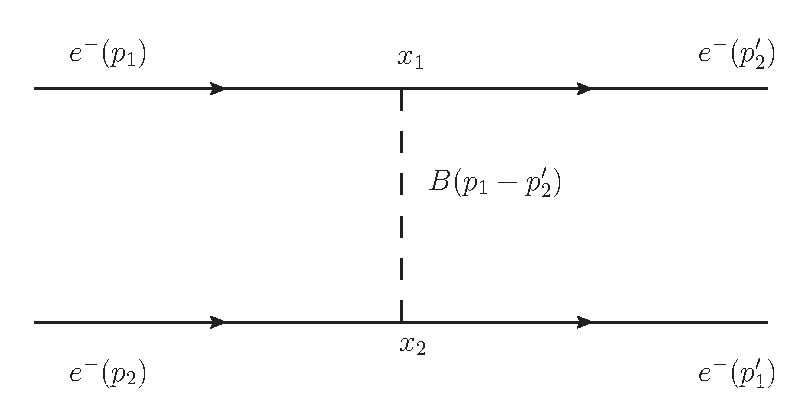
\includegraphics{scattering} %noinstiki
 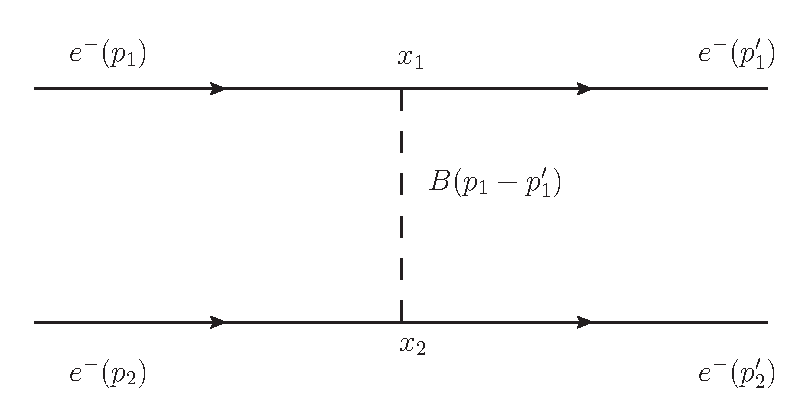
\includegraphics{scattering2} %noinstiki
  \caption{fermion scattering} %noinstiki
  \label{fig:sct} %noinstiki
\end{figure} %noinstiki
Since
\begin{align}
  \Delta_F(q)=\frac{1}{q^2-m^2}
\end{align}
In the limit $q^2\ll m^2$
\begin{align}
  \Delta_F=-\frac{1}{m^2}
\end{align}
\begin{align}
  \mathcal{M}_{fi}=&\frac{h^2}{m^2}\left[
\bar{u}^\alpha(\mathbf{p}_2')u^\alpha(\mathbf{p}_1)\bar{u}^\beta(\mathbf{p}_1')u^\beta(\mathbf{p}_2)
-\bar{u}^\alpha(\mathbf{p}_1')u^\alpha(\mathbf{p}_1)\bar{u}^\beta(\mathbf{p}_2')u^\beta(\mathbf{p}_2)
\right]\nonumber\\
=&\frac{h^2}{m^2}\left[
\bar{u}(\mathbf{p}_2')u(\mathbf{p}_1)\bar{u}(\mathbf{p}_1')u(\mathbf{p}_2)
-\bar{u}(\mathbf{p}_1')u(\mathbf{p}_1)\bar{u}(\mathbf{p}_2')u(\mathbf{p}_2)
\right]
\end{align}
For one interaction of type $\overline{\psi}\Gamma\psi$ we should have
\begin{align}
  \mathcal{M}_{fi}=\frac{h^2}{m^2}\left[
\bar{u}(\mathbf{p}_2')\Gamma u(\mathbf{p}_1)\bar{u}(\mathbf{p}_1')\Gamma u(\mathbf{p}_2)
-\bar{u}(\mathbf{p}_1')\Gamma u(\mathbf{p}_1)\bar{u}(\mathbf{p}_2')\Gamma u(\mathbf{p}_2)
\right]
\end{align}
For the interaction of a fermion pair with $W_\mu^\pm$, we know from
the standard model Lagrangian \cite{lsm}, that
\begin{align}
  \frac{g^2}{2\sqrt{2}}\overline{\psi}\gamma^\mu(1-\gamma_5)\psi
\end{align}
Therefore in this case
\begin{align}
  \Gamma=\gamma^\mu(1-\gamma_5)
\end{align}
For $p\ll M_W^2$ the analysis is similar to the previous one with
\begin{align}
   \bcontraction{\,}{W^\mu}{(x_1)}{W^\nu}
\,W^\mu(x_1)W^\nu(x_2)=&\langle0|T\{W^\mu(x_1)W^\nu(x_2)\}|0\rangle\nonumber\\
\approx&\int\frac{d^4q}{(2\pi)^4}\frac{g^{\mu\nu}}{M_W^2}e^{-i q\cdot(x_1-x_2)}
\end{align}

For the process 
\begin{align}
  e^-(p)+\nu_\mu(k)\to\mu^-(p')+\nu_e(k')
\end{align}
the global coupling for $p\ll M_W^2$ is
\begin{align}
  \frac{g^2}{8M_W^2}=&\frac{G_F}{\sqrt{2}}
\end{align}

After the replacement $G_F/\sqrt{2}\equiv h^2/m^2$, we have
\begin{align}
  \label{eq:101f}
  S^{(2)}_{fi}=i(2\pi)^4\delta^{4}\left(p_1+p_2-p'_1-p'_2\right)
  \frac{1}{\sqrt{2E_1 V}}\frac{1}{\sqrt{2E_2 V}}
  \frac{1}{\sqrt{2E_1' V}}\frac{1}{\sqrt{2E_2' V}}
  \mathcal{M}_{fi}
\end{align}
where
\begin{align}
  \mathcal{M}_{fi}=\frac{G_F}{\sqrt{2}}
\bar{u}_{\nu_e}(\mathbf{p}'_2)\Gamma u_e(\mathbf{p}_1)\bar{u}_\mu(\mathbf{p}'_1)\Gamma u_{\nu_\mu}(\mathbf{p_2})
\end{align}
The corresponding Feynman diagram is shown in Fig.~\ref{fig:sw}
\begin{figure} %noinstiki
  \centering %noinstiki
  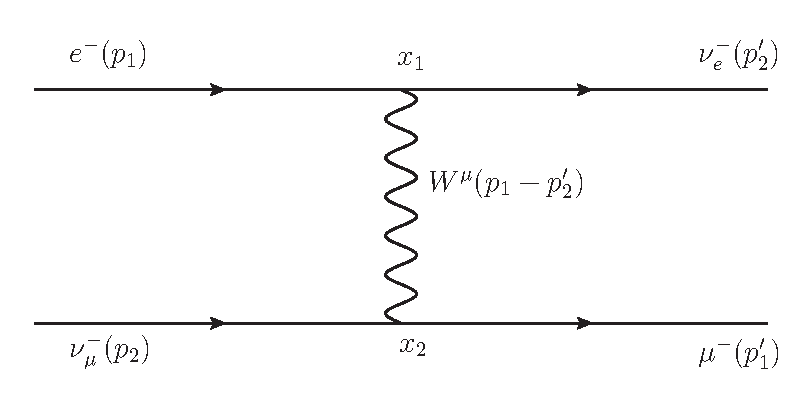
\includegraphics{scatteringw} %noinstiki
  \caption{scattering with four fermions} %noinstiki
  \label{fig:sw} %noinstiki
\end{figure} %noinstiki
Therefore we have

\begin{align}
  \mathcal{M}_{fi}=\frac{G_F}{\sqrt{2}}
\bar{u}_{\nu_e}(\mathbf{p}_2')\gamma^\mu(1-\gamma_5)u_e(\mathbf{p_1})
\bar{u}_\mu(\mathbf{p}_1')\gamma_\mu(1-\gamma_5)u_{\nu_\mu}(\mathbf{p_2})
\end{align}
We now must sqaure the scattering amplitude, $\mathcal{M}$, and summing up over final spin states, and averaging over the intial spin states, as we did in Eq.~\eqref{eq:81f}. The result that will be obtained in detail in Chapter~\ref{cha:three-body-decays} for the muon--decay is
\begin{align}
  \label{eq:102f}
  \overline{|\mathcal{M}|^2}=64\,G_F^2\,(p_1\cdot p_2)(p_1'\cdot p_2')
\end{align}

From Eq.~\eqref{eq:74f}
\begin{align}
  \label{eq:103f}
  \frac{d\sigma}{d\Omega}=\frac{1}{64\pi^2s}\left(\frac{s-m_\mu^2}{s-m_e^2}\right)\overline{|\mathcal{M}|^2}
\end{align}

The center of mass (CM) frame is defined by the condition in Eq.~\eqref{eq:55f}:
\begin{align}
  \mathbf{p}_1+\mathbf{p}_2=0
\end{align}
The $\delta$--function in Eq.~\eqref{eq:101f}
\begin{align}
  \delta^{(4)}(p_1+p_2-p_1'-p_2')=\delta^{(3)}(\mathbf{p}_1+\mathbf{p}_2-\mathbf{p}_1'-\mathbf{p}_2')
\delta(E_1+E_2-E_1'-E_2')
\end{align}

implies
\begin{align}
  \label{eq:157f}
  \mathbf{p}_1+\mathbf{p}_2-\mathbf{p}_1'-\mathbf{p}_2'=0 \overset{\text{CM}}{\Rightarrow}
  \begin{cases}
    \mathbf{p}_1=-\mathbf{p}_2\\
    \mathbf{p}_1'=-\mathbf{p}_2'\\
  \end{cases}
\end{align}
Moreover
\begin{align}
  \sqrt{s}=E_1+E_2
\end{align}
In the CM frame
\begin{align}
\label{eq:104f}
s=&\left(E_1+E_2\right)^2\nonumber\\
=&\left(\sqrt{\mathbf{p}_1^2+m_1^2}+\sqrt{\mathbf{p}_2^2+m_2^2}\right)^2\nonumber\\
=&\left(\sqrt{\mathbf{p}_1^2+m_e^2}+\sqrt{\mathbf{p}_1^2+m_{\nu_e}^2}\right)^2
\end{align}
Therefore
\begin{align}
  \label{eq:105f}
  E_2=|\mathbf{p}_1|
\end{align}
We already have the expression for $|\mathbf{p}_1|$ as given in eq.~\eqref{eq:71f}. In this case $m_2=0$, and $m_1=m_e$, so that
\begin{align}
  \label{eq:158f}
  |\mathbf{p}_1|=\frac{s-m_e^2}{2\sqrt{s}}
\end{align}

From \eqref{eq:105f}
\begin{align}
  \sqrt{s}=&E_1+E_2\nonumber\\
  =&E_1+|\mathbf{p}_1|
\end{align}
\begin{align}
  \label{eq:106f}
  E_1=&\sqrt{s}-|\mathbf{p}_1|\nonumber\\
  =&\sqrt{s}+\frac{-s+m_e^2}{2\sqrt{s}}\nonumber\\
  =&\frac{2s-s+m_e^2}{2\sqrt{s}}\nonumber\\
  =&\frac{s+m_e^2}{2\sqrt{s}}
\end{align}
Then, by using Eqs.~\eqref{eq:157f}, \eqref{eq:105f} and \eqref{eq:158f}, and~\eqref{eq:106f},  we have
\begin{align}
  p_1\cdot p_2=&E_1E_2-\mathbf{p}_1\cdot\mathbf{p}_2\nonumber\\
  =&E_1|\mathbf{p}_1|+\mathbf{p}_1^2\nonumber\\
=&\frac{(s-m_e^2)(s+m_e^2)}{4s}+\frac{(s-m_e^2)^2}{4s}\nonumber\\
=&\frac{(s-m_e^2)}{4s}(s+m_e^2+s-m_e^2)\nonumber\\
=&\frac{1}{2}(s-m_e^2) 
\end{align}
As $p_2^2={p_2'}^2=0$, we have from $\delta$--function
\begin{align}
  (p_1+p_2)^2=&(p_1'+p_2')^2\nonumber\\
  (p_1+p_2)^2=&(p_1'+p_2')^2\nonumber\\
  p_1^2+2p_1\cdot p_2+p_2^2=&{p_1'}^2+2p_1'\cdot p_2'+{p_2'}^2\nonumber\\
  p_1^2+2p_1\cdot p_2=&{p_1'}^2+2p_1'\cdot p_2'\nonumber\\
  m_e^2+2p_1\cdot p_2=&m_\mu^2+2p_1'\cdot p_2'
\end{align}
\begin{align}
  p_1'\cdot p_2'=p_1\cdot p_2-\frac{1}{2}(m_\mu^2-m_e^2)
\end{align}
\begin{align}
  p_1'\cdot p_2'=\frac{1}{2}(s-m_\mu^2) 
\end{align}
Replacing back in Eq.~\eqref{eq:102f} and then in Eq.~\eqref{eq:103f} we have
\begin{align}
  \frac{d\sigma}{d\Omega}=\frac{1}{64\pi^2s}\left(\frac{s-m_\mu^2}{s-m_e^2}\right)
64G_F^2\frac{1}{2}(s-m_e^2)\frac{1}{2}(s-m_\mu^2)
\end{align} 
\begin{align}
    \frac{d\sigma}{d\Omega}=\frac{G_F^2}{4\pi^2}\frac{(s-m_\mu^2)^2}{s}
\end{align}
\begin{align}
\sigma  =\frac{G_F^2}{\pi}\frac{(s-m_\mu^2)^2}{s}
\end{align}
Note that $\sigma\propto s$.
%\left(\right)
%\left[\right]


%%% Local Variables: 
%%% mode: latex
%%% TeX-master: "beyond"
%%% End: 


%instiki:category: QuantumFieldTheory
\chapter{Three body decays}
\label{cha:three-body-decays} %noinstiki
%instiki:
%instiki:***
%instiki:
%instiki:[[Beyond|Contents]]
%instiki:
%instiki:***
%instiki:
%instiki:* [Muon decay](#mu-decay)
%instiki: 
%instiki:* [three body decays in radiative seesaw](#three-body-decays)
%instiki:
%instiki:* [Sample point](#sample-point)
%instiki:
%instiki:* [Preliminary discussion](#prel-disc)
%instiki:

\section{Muon decay}
\label{sec:mu-decay} 

For a three body decay we have from eq.~\eqref{eq:76}
\begin{align}
  \label{eq:107}
  d\Gamma =& \frac{1}{(2\pi)^5}\frac{1}{2M}\left|\mathcal{M}\right|^2 \delta^4(P-p_1-p_2-p_3)\frac{d^3 p_1}{2E_1}
\frac{d^3 p_2}{2E_2}\frac{d^3 p_3}{2E_3}\nonumber\\
  =& \frac{1}{(2\pi)^5}\frac{1}{2M}\frac{d^3 p_1}{2E_1}\int\left|\mathcal{M}\right|^2 \delta^4(P-p_1-p_2-p_3)
\frac{d^3 p_2}{2E_2}\frac{d^3 p_3}{2E_3}\nonumber\\
\end{align}

\subsection{Amplitude estimation}
\label{sec:amplitude-estimation}
Since $\mathcal{M}$ is dimensionless, the amplitude averaged over spins for $\mu$ decay must be
\begin{equation}
  |\mathcal{M}|^2=C G_F^2 m_\mu^4\,.
\end{equation}
We use
\begin{equation}
  C=\frac{1}{2}(2\times2\times1\times1)=2
\end{equation}
The first factor is for the initial average and the factor are for the number of spin states of $\mu$, $e$ and the two neutrinos. 


Consider first the integral
\begin{align}
  \int \delta^4(P-p_1-p_2)
\frac{d^3 p_1}{2E_1}\frac{d^3 p_2}{2E_2}=&\int\delta(E-E_1-E_2)
\delta^3(\mathbf{P}-\mathbf{p}_1-\mathbf{p}_2)\frac{d^3 p_1}{2E_1}\frac{d^3 p_2}{2E_2}\nonumber\\
  =&\int\delta(E-E_1-E_2)
\frac{d^3 p_2}{4E_1 E_2}\int\delta^3(\mathbf{P}-\mathbf{p}_1-\mathbf{p}_2){d^3 p_1}\nonumber\\
  =&\int\delta(E-E_1-E_2)
\frac{d^3 p_2}{4E_1 E_2}\int\delta^3(\mathbf{p}_1+\mathbf{p}_2-\mathbf{P}){d^3 p_1}\nonumber\\
  =&\int\delta(E-E_1-E_2)
\frac{d^3 p_2}{4E_1 E_2}\int\delta^3[\mathbf{p}_1-(\mathbf{P}-\mathbf{p}_2)]{d^3 p_1}
\end{align}
using
\begin{align}
  \int\delta(x-x_0)dx=1
\end{align}
we have
\begin{align}
  \label{eq:108}
    \int \delta^4(P-p_1-p_2)
\frac{d^3 p_1}{2E_1}\frac{d^3 p_2}{2E_2}=&
\int\delta(E-E_1-E_2)\frac{d^3 p_2}{4E_1 E_2}\nonumber\\
    \int \delta^4(P-p_1-p_2)
\frac{d^3 p_1}{2E_1}\frac{d^3 p_2}{2E_2}=&
\int\delta(E-E_1-E_2)\frac{\mathbf{p}_2^2\,d|\mathbf{p}_2|d\Omega}{4E_1 E_2}
\end{align}
Since $|\mathbf{p}_1|=|\mathbf{p}_2|$ we have
\begin{align}
  E=E_1+E_2=&(m_1^2+\mathbf{p}_1^2)^{1/2}+(m_2^2+\mathbf{p}_2^2)^{1/2}\nonumber\\
  =&(m_1^2+\mathbf{p}_2^2)^{1/2}+(m_2^2+\mathbf{p}_2^2)^{1/2}
\end{align}
differentiating this equation with respect to $\mathbf{p}_2$
\begin{align}
  \frac{d E}{d|\mathbf{p}_2|}=&\frac{1}{2}\left(
\frac{2|\mathbf{p}_2|}{(m_1^2+\mathbf{p}_2^2)^{1/2}}+
\frac{2|\mathbf{p}_2|}{(m_2^2+\mathbf{p}_2^2)^{1/2}}\right)\nonumber\\
=&|\mathbf{p}_2|\left(\frac{1}{E_1}+\frac{1}{E_2}\right)\nonumber\\
  =&|\mathbf{p}_2|\left(\frac{E_1+E_2}{E_1 E_2}\right)
\end{align} 
Therefore
\begin{align}
  d|\mathbf{p}_2|=\frac{d E}{|\mathbf{p}_2|}\left(\frac{E_1 E_2}{E_1+E_2}\right)
\end{align}
replacing back in eq.~(\ref{eq:108})
\begin{align}
      \int \delta^4(P-p_1-p_2)\frac{d^3 p_1}{2E_1}\frac{d^3 p_2}{2E_2}
      =&\int\frac{d E}{|\mathbf{p}_2|}\,\delta(E-E_1-E_2)\frac{\mathbf{p}_2^2\,d\Omega}{4E_1 E_2}
      \left(\frac{E_1 E_2}{E_1+E_2}\right)\nonumber\\
      =&\int d E\,\delta(E-E_1-E_2)\frac{|\mathbf{p}_2|\,d\Omega}{4(E_1+E_2)}\nonumber\\
      =&  \int\frac{|\mathbf{p}_2|}{4 E}d\Omega
\end{align}
For a relativistic particle $|\mathbf{p}_2|\approx E_2=E/2$ and
\begin{align}
  \int \delta^4(P-p_1-p_2)\frac{d^3 p_1}{E_1}\frac{d^3 p_2}{E_2}=2\pi
\end{align}
Applying this result to eq.~(\ref{eq:107}) we have
\begin{align}
    d\Gamma =& \frac{1}{(2\pi)^5}\frac{1}{2M}\frac{d^3 p_1}{2E_1}\int\left|\mathcal{M}\right|^2 \delta^4(P-p_1-p_2-p_3)
\frac{d^3 p_2}{2E_2}\frac{d^3 p_3}{2E_3}\nonumber\\
=&\frac{1}{(2\pi)^5}\frac{1}{2M}\frac{d^3 p_1}{8E_1}\left|\mathcal{M}\right|^2\int \delta^4(P-p_1-p_2-p_3)
\frac{d^3 p_2}{E_2}\frac{d^3 p_3}{E_3}\nonumber\\
=&\frac{1}{(2\pi)^5}\frac{1}{2M}\frac{d^3 p_1}{8E_1}\left|\mathcal{M}\right|^2(2\pi)\nonumber\\
  =&\frac{G_F^2m_\mu^4}{8(2\pi)^4 m_\mu E_1} \mathbf{p}_1^2 d|\mathbf{p}_1|\int d\Omega\nonumber\\
  \approx&\frac{G_F^2m_\mu^3}{8(2\pi)^4  E_1} E_1^2 d E_1(4\pi)\nonumber\\
  \approx&\frac{G_F^2m_\mu^3}{4(2\pi)^3} E_1 d E_1
\end{align}
As the maximum value  of $E_1$ is $m_\mu/2$
\begin{align}
  \Gamma\approx&\frac{G_F^2m_\mu^3}{4(2\pi)^3} \int_0^{m_\mu/2}E_1 d E_1\nonumber\\
   =&\frac{G_F^2m_\mu^3}{4(2\pi)^3} \frac{m_\mu^2}{8}\,,
\end{align}
or
\begin{equation}
  \Gamma=\frac{3}{4}\frac{G_F^2m_\mu^5}{192\pi^3}\,.
\end{equation}

\subsection{Amplitude calculation}
\label{sec:ampl-calc}
The Standard Model Lagrangian includes
\begin{align}
  \mathcal{L}=&-\frac{\sqrt{2}g}{2}(\overline{\nu_e}_L\gamma^\mu e_L W_\mu^++\bar{e}_L\gamma^\mu{\nu_e}_L W_\mu^-+\overline{\nu_\mu}_L\gamma^\mu\mu_L W_\mu^++\bar{\mu}_L\gamma^\mu{\nu_\mu}_L W_\mu^-)\nonumber\\
=&-\frac{g}{\sqrt{2}}(\overline{\nu_e}\gamma^\mu P_L e W_\mu^++\bar{e}\gamma^\mu P_L{\nu_e} W_\mu^-+\overline{\nu_\mu}\gamma^\mu P_L\mu W_\mu^++\bar{\mu}\gamma^\mu P_L{\nu_\mu} W_\mu^-)\nonumber\\
=&-\frac{g}{2\sqrt{2}}(\overline{\nu_e}\gamma^\mu (1-\gamma_5) e W_\mu^++\bar{e}\gamma^\mu (1-\gamma_5){\nu_e} W_\mu^-+\overline{\nu_\mu}\gamma^\mu (1-\gamma_5)\mu W_\mu^++\bar{\mu}\gamma^\mu (1-\gamma_5){\nu_\mu} W_\mu^-)
\end{align}
where
\begin{align}
  \label{eq:109}
  (\overline{\nu_e}\gamma^\mu P_L e W_\mu^+)^\dagger&=e^\dagger{\gamma^\mu P_L}^\dagger(\overline{\nu_e})^\dagger W_\mu^-
  =e^\dagger P_L{\gamma^\mu}^\dagger\gamma^0\nu_e W_\mu^-=e^\dagger\gamma^0\gamma^0{\gamma^\mu}^\dagger P_R\gamma^0\nu_e W_\mu^-\nonumber\\
  &=\bar{e}\gamma^0{\gamma^\mu}^\dagger\gamma^0P_L\nu_e W_\mu^-=\bar{e}\gamma^\mu P_L\nu_e W_\mu^-
\end{align}
We can build the effective Lagrangian

Applying the Feynman rules to the diagram in fig. 
\ref{fig:1} %noinstiki
we have the amplitude
\begin{align}
  \mathcal{M}=\frac{-ig^2}{8}\bar{u}_3\gamma_\mu(1-\gamma_5)u_1\left(\frac{-g^{\mu\nu}+q^\mu q^\nu/M_W^2}{q^2-M_W^2}\right)\bar{u}_4\gamma_\nu(1-\gamma_5)v_2
\end{align}
where $u$ ($v$) is for an incoming particle and $\bar{u}$ ($\bar{v}$) is for an ongoing particle (antiparticle).

\begin{figure} %noinstiki
  \centering %noinstiki
  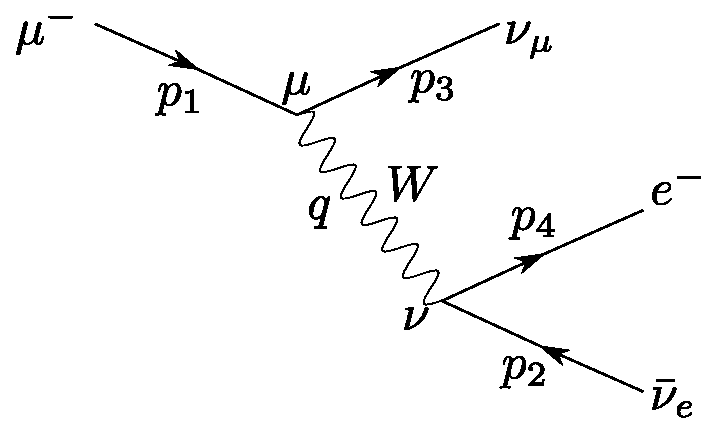
\includegraphics{muon_decay}%noinstiki
  \caption{Tree level diagram for muon decay } %noinstiki
  \label{fig:1} %noinstiki
\end{figure} %noinstiki


The Dirac equations for spinors $u$ and $v$ are
\begin{align}
  (\cancel{p}-m)u&=0&(\cancel{p}+m )v&=0\nonumber\\
  \bar{u}(\cancel{p}-m)&=0&\bar{v}(\cancel{p}+m )&=0\,.
\end{align}
In this way
\begin{align}
  \frac{1}{M_W^2}\gamma_\mu q^\mu(1-\gamma_5)u_1 \bar{u}_4\gamma_\nu q^\nu(1-\gamma_5)
  =&\frac{1}{M_W^2}(1+\gamma_5)\cancel{q}u_1 \bar{u}_4\cancel{q}(1-\gamma_5)\nonumber\\
  =&-\frac{m_\mu m_e}{M_W^2}(1+\gamma_5)u_1 \bar{u}_4(1-\gamma_5)\,
\end{align}
the term in $q^\mu q^\nu$ can be safely neglected. The term $q^2$ is $m_\mu^2$ is small compared with $m_W^2$. Therefore
\begin{align}
  \mathcal{M}=&\frac{-i g^2}{8M_W^2}\bar{u}_3\gamma_\mu(1-\gamma_5)u_1\bar{u}_4\gamma^\mu(1-\gamma_5)v_2\nonumber\\
  =&\frac{-i G_F}{\sqrt{2}}\bar{u}_3\gamma_\mu(1-\gamma_5)u_1\bar{u}_4\gamma^\mu(1-\gamma_5)v_2
\end{align}
$\mathcal{M}$ is a dimensionless scalar. The relevant coupling is
\begin{equation}
  \frac{g^2}{8M_W^2}=\frac{G_F}{\sqrt{2}}\,.
\end{equation}
The conjugate is, following  the same steps that in eq.~\eqref{eq:109}
\begin{align}
  \mathcal{M}^*=&\frac{i g^2}{8M_W^2}\left[\bar{u}_3\gamma_\mu(1-\gamma_5)u_1\right]^\dagger
  \left[\bar{u}_4\gamma^\mu(1-\gamma_5)v_2\right]^\dagger\nonumber\\
   \mathcal{M}^*=&\frac{i g^2}{8M_W^2}\left[\bar{u}_1\gamma_\mu(1-\gamma_5)u_3\right]
  \left[\bar{v}_2\gamma^\mu(1-\gamma_5)u_4\right]\,.
\end{align}
Multiplying $\mathcal{M}$ and $\mathcal{M}^*$ we have
\begin{align}
  \label{eq:110}
  |\mathcal{M}|^2=&\frac{g^4}{64 M_W^4}\left[\bar{u}_3\gamma_\mu(1-\gamma_5)u_1\bar{u}_1\gamma_\nu(1-\gamma_5)u_3\right]\nonumber\\
  &\times\left[\bar{u}_4\gamma^\mu(1-\gamma_5)v_2\bar{v}_2\gamma^\nu(1-\gamma_5)u_4\right]\nonumber\\
  =&\frac{g^4}{64 M_W^4}L_{\mu\nu}M^{\mu\nu}
\end{align}
where
\begin{align}
   L_{\mu\nu}=&\left[\bar{u}_{3\alpha}\gamma_\mu^{\alpha\beta}(1-\gamma_5)_{\beta\gamma}u_1^\gamma\bar{u}_{1\delta}\gamma_\nu^{\delta\epsilon}(1-\gamma_5)_{\epsilon\eta}u_3^\eta\right]\nonumber\\
  M^{\mu\nu}=&\left[\bar{u}_4^\alpha\gamma^\mu_{\alpha\beta}(1-\gamma_5)^{\beta\gamma}v_{2\gamma}\bar{v}_2^\delta\gamma^\nu_{\delta\epsilon}(1-\gamma_5)^{\epsilon\eta}u_{4\eta}\right]
\end{align}
\begin{align}
     L_{\mu\nu}=&\left[u_3^\eta\bar{u}_{3\alpha}\gamma_\mu^{\alpha\beta}(1-\gamma_5)_{\beta\gamma}u_1^\gamma\bar{u}_{1\delta}\gamma_\nu^{\delta\epsilon}(1-\gamma_5)_{\epsilon\eta}\right]\nonumber\\
     =&\left[(u_3\bar{u}_{3})_{\eta\alpha}\gamma_\mu^{\alpha\beta}(1-\gamma_5)_{\beta\gamma}(u_1\bar{u}_{1})_{\gamma\delta}\gamma_\nu^{\delta\epsilon}(1-\gamma_5)_{\epsilon\eta}\right]\nonumber\\
     =&\operatorname{Tr}\left[(u_3\bar{u}_{3})\gamma_\mu(1-\gamma_5)(u_1\bar{u}_{1})\gamma_\nu(1-\gamma_5)\right]
\end{align}
Using
\begin{align}
  \label{eq:111}
 \sum_su(p,s)\bar{u}(p,s)&=(\cancel{p}+m)& \sum_sv(p,s)\bar{v}(p,s)&=(\cancel{p}-m)
\end{align}
\begin{align}
  \sum_s L_{\mu\nu}=&\operatorname{Tr}\left[(\cancel{p}_3)\gamma_\mu(1-\gamma_5)(\cancel{p}_1+m_\mu)\gamma_\nu(1-\gamma_5)\right]\nonumber\\
  =&p_3^\alpha\operatorname{Tr}\left[\gamma_\alpha\gamma_\mu(1-\gamma_5)(p_1^\beta\gamma_\beta+m_\mu)\gamma_\nu(1-\gamma_5)\right]\nonumber\\
  =&p_3^\alpha\operatorname{Tr}\left[(\gamma_\alpha\gamma_\mu-\gamma_\alpha\gamma_\mu\gamma_5)(p_1^\beta\gamma_\beta\gamma_\nu(1-\gamma_5)+m_\mu\gamma_\nu(1-\gamma_5))\right]\nonumber\\
  =&p_3^\alpha\operatorname{Tr}\left[p_1^\beta\gamma_\alpha\gamma_\mu\gamma_\beta\gamma_\nu(1-\gamma_5)-p_1^\beta\gamma_\alpha\gamma_\mu\gamma_5\gamma_\beta\gamma_\nu(1-\gamma_5)\right.\nonumber\\
&\left.+m_\mu\gamma_\alpha\gamma_\mu\gamma_\nu(1-\gamma_5)-m_\mu\gamma_\alpha\gamma_\mu\gamma_5\gamma_\nu(1-\gamma_5)\right]\nonumber\\
  =&p_3^\alpha\operatorname{Tr}\left[p_1^\beta\gamma_\alpha\gamma_\mu\gamma_\beta\gamma_\nu-p_1^\beta\gamma_\alpha\gamma_\mu\gamma_\beta\gamma_\nu\gamma_5-p_1^\beta\gamma_\alpha\gamma_\mu\gamma_5\gamma_\beta\gamma_\nu
+p_1^\beta\gamma_\alpha\gamma_\mu\gamma_5\gamma_\beta\gamma_\nu\gamma_5\right.\nonumber\\
&\left.+m_\mu\gamma_\alpha\gamma_\mu\gamma_\nu-m_\mu\gamma_\alpha\gamma_\mu\gamma_\nu\gamma_5-m_\mu\gamma_\alpha\gamma_\mu\gamma_5\gamma_\nu+m_\mu\gamma_\alpha\gamma_\mu\gamma_5\gamma_\nu\gamma_5\right]
\end{align}
as the trace of an odd number of $\gamma$--matrices is zero, we have
\begin{align}
  \sum_s L_{\mu\nu}=&p_3^\alpha p_1^\beta\operatorname{Tr}\left[\gamma_\alpha\gamma_\mu\gamma_\beta\gamma_\nu-\gamma_\alpha\gamma_\mu\gamma_\beta\gamma_\nu\gamma_5-\gamma_\alpha\gamma_\mu\gamma_\beta\gamma_\nu\gamma_5
+\gamma_\alpha\gamma_\mu\gamma_\beta\gamma_\nu\gamma_5^2\right]\nonumber\\
=&2 p_3^\alpha p_1^\beta\operatorname{Tr}\left[\gamma_\alpha\gamma_\mu\gamma_\beta\gamma_\nu(1-\gamma_5)\right]
\end{align}
Similarly
\begin{align}
  \sum_s M^{\mu\nu}=2 p_{4\delta}p_{2\epsilon}\operatorname{Tr}\left[\gamma^\delta\gamma^\mu\gamma^\epsilon\gamma^\nu(1-\gamma_5)\right]
\end{align}
substituting back in eq.~(\ref{eq:110}) we have,
\begin{align}
  \label{eq:112}
   |\mathcal{M}|^2=&\frac{g^4}{64 M_W^4}4p_3^\alpha p_1^\beta p_{4\delta}p_{2\epsilon}
   \operatorname{Tr}\left[\gamma_\alpha\gamma_\mu\gamma_\beta\gamma_\nu(1-\gamma_5)\right]
   \operatorname{Tr}\left[\gamma^\delta\gamma^\mu\gamma^\epsilon\gamma^\nu(1-\gamma_5)\right]\nonumber\\
   =&\frac{g^4}{64 M_W^4}4p_3^\alpha p_1^\beta p_{4\delta}p_{2\epsilon}(64\delta^\alpha_\delta\delta^\beta_\epsilon)\nonumber\\
  =&\frac{g^4}{64 M_W^4}4\times64(p_3\cdot p_4)(p_1\cdot p_2)\nonumber\\
  =&\frac{4g^4}{M_W^4}(p_3\cdot p_4)(p_1\cdot p_2)\nonumber\\
  =&4\left(8\frac{g^2}{8M_W^2}\right)^2(p_3\cdot p_4)(p_1\cdot p_2)\nonumber\\
  =&4\left(8\frac{G_F}{\sqrt{2}}\right)^2(p_3\cdot p_4)(p_1\cdot p_2)\nonumber\\
  =&128\, G_F^2(p_3\cdot p_4)(p_1\cdot p_2)\nonumber\\
  =&256\frac{G_F^2}{{2}}(p_3\cdot p_4)(p_1\cdot p_2)\,.
\end{align}
The demonstration of the used Tr$\times$Tr identity can be found in Appendix B. of \cite{PeterRenton}.

The spin--averaged differential decay width for $\mu^-\to\nu_\mu e^-\bar{\nu}_e$ is
\begin{align}
  \label{eq:113}
  d\Gamma =& \frac{1}{(2\pi)^5}\frac{1}{2E_1}\frac{d^3 p_3}{2E_3}
\left(\frac{1}{2}\sum\left|\mathcal{M}\right|^2\right) \delta^4(p_1-p_2-p_3-p_4)
\frac{d^3 p_2}{2E_2}\frac{d^3 p_4}{2E_4}\nonumber\\
 =&\frac{1}{2E_1}\frac{1}{2}\sum\left|\mathcal{M}\right|^2\frac{1}{(2\pi)^5}\frac{d^3 p_2}{8E_2}
  \delta^4(p_1-p_2-p_3-p_4)\frac{d^3 p_3}{E_3}\frac{d^3 p_4}{E_4}\nonumber\\
=&\frac{1}{2}\frac{4g^4}{M_W^4}\frac{1}{(2\pi)^52E_1}(p_1\cdot p_2)(p_3\cdot p_4)\frac{d^3 p_2}{2E_2}
  \delta^4(p_1-p_2-p_3-p_4)\frac{d^3 p_3}{2E_3}\frac{d^3 p_4}{2E_4}\nonumber\\
  =&\frac{2g^4}{16 (2\pi)^5 M_W^4 E_1 E_4}p_1^\beta p_4^\alpha d^3p_4 I_{\alpha\beta}
\end{align}
where the covariant integral $I_{\alpha\beta}$ on the neutrino momentum is
\begin{align}
  \label{eq:114}
  I_{\alpha\beta}=\int p_{3\alpha}p_{2\beta}\delta^4(p-p_2-p_3)\frac{d^3 p_2}{E_2}\frac{d^3 p_3}{E_3}\,.
\end{align}
The variable $p$ in ec.~\eqref{eq:114} is defined as $p=p_1-p_4=p_2+p_3$. Moreover
\begin{align}
  \label{eq:115}
  p^2=&p_2^2+p_3^2+2p_2\cdot p_3\nonumber\\
  =&m_{\nu_e}^2+m_{\nu_\mu}^2+2p_2\cdot p_3\nonumber\\
  \approx&2p_2\cdot p_3\nonumber\\
g_{\alpha\beta}p^\alpha p^\beta=&2 g_{\alpha\beta}p_3^\alpha p_2^\beta\nonumber\\
p^\alpha p^\beta=&2p_3^\alpha p_2^\beta\,.
\end{align}
$I_{\alpha\beta}$ must have the form
\begin{align}
  \label{eq:116}
  I_{\alpha\beta}=g_{\alpha\beta}A(p^2)+p_\alpha p_\beta B(p^2)\,.
\end{align}
Defining the itegral $I$ as follows
\begin{equation}
  I=\int\delta^4(p-p_2-p_3)\frac{d^3 p_2}{E_2}\frac{d^3 p_3}{E_3}\,,
\end{equation}
Since
\begin{align}
  m_\nu^2\approx0=&E_\nu^2-\mathbf{p}_\nu^2\nonumber\\
E_\nu^2=&\mathbf{p}_\nu^2
\end{align}
and in addition the integral $I$ is covariant, we choose to evaluate it in the rest frame of the two neutrinos
$|\mathbf{p}_2|=|\mathbf{p}_3|$, which implies $E_2=E_3$.
\begin{align}
  I=&\int\delta(E-E_2-E_3)\delta^3(\mathbf{p}-\mathbf{p}_2-\mathbf{p}_3)\frac{d^3 p_2}{E_2}\frac{d^3 p_3}{E_3}\nonumber\\
    =&\int\delta(E-E_2-E_3)\frac{d^3 p_2}{E_2E_3}\underbrace{\int\delta^3(\mathbf{p}-\mathbf{p}_2-\mathbf{p}_3)d^3 p_3}_{=1}\nonumber\\
    =&\int\frac{\delta(E-2E_2)}{E_2^2}\mathbf{p}_2^2 d|\mathbf{p}_2|d\Omega\nonumber\\
    =&\int\frac{\delta(E-2E_2)}{E_2^2}E_2^2 dE_2 (4\pi)\nonumber\\
    =&4\pi\int\delta\left(2\left(E_2-\frac{E}{2}\right)\right) dE_2 \nonumber\\
    =&4\pi\frac{1}{2}\int\delta\left(E_2-\frac{E}{2}\right) dE_2 \nonumber\\
    =&2\pi
\end{align}

then multiplying (6.13) by $g^{\alpha\beta}$ and $p^\alpha p^\beta$ successively gives, using eq.~\eqref{eq:115}
\begin{equation}
  g^{\alpha\beta}I_{\alpha\beta}=4 A +p^2 B=\int p_{3}\cdot
  p_{2}\delta^4(p-p_2-p_3)\frac{d^3 p_2}{E_2}\frac{d^3
    p_3}{E_3}\nonumber =\frac{p^2}{2}I=\pi p^2\nonumber
\end{equation}

In order to compute $p^\alpha p^\beta I_{\alpha\beta}$, we make use of
the fact that it is a Lorentz invariant quantity, so that we may
evaluate it in any reference frame. In particular, we can evaluate it
in the rest frame of the neutrinos involved in this process. This
means that $p=p_2+p_3=(p^0,\mathbf{0})$ and $E_2=E_3$
\begin{align}
p^\alpha p^\beta I_{\alpha\beta}&=p^2 A+p^4 B\\ 
&=p^\alpha
p^\beta\int\frac{d^3 p_2}{E_2}\frac{d^3 p_3}{E_3}
p_{3\alpha}p_{2\beta}\delta^4(p-p_2-p_3) \nonumber\\
&=\int \frac{d^3
  p_2}{E_2}\frac{d^3 p_3}{E_3} E_3p^0E_2p^0\delta^4(p-p_2-p_3)\nonumber\\
&=(p^0)^2\int d^3 p_2d^3 p_3
\delta^4(p-p_2-p_3)\\
&=(p^0)^2\int d^3 p_2 \delta(p^0-2E_2)\nonumber\\
&=(p)^2\int d E_2 E_2^2 d\Omega
\frac{1}{2}\delta(\frac{p^0}{2}-E_2) 
=4\pi\frac{p^2}{2}\left(\frac{p^2}{2}\right)^2 \nonumber\\
&=\frac{\pi p^4}{2}
\end{align}
where the usual tricks have been used to simplify the integrals, using
the delta function inside.

Therefore
\begin{equation}
  A=\frac{p^2}{4}(\pi-B)
\end{equation}
\begin{align}
  \frac{p^4}{4}(\pi-B)+p^4B=&\frac{\pi p^4}{2}\nonumber\\
    \frac{\pi}{4} -\frac{B}{4}+B=&\frac{\pi}{2}\nonumber\\
    \frac{3B}{4}=&\frac{\pi}{4}\nonumber\\
    B=&\frac{\pi}{3}
\end{align}
\begin{align}
  A=&\frac{p^2}{4}(\pi-\frac{\pi}{3})\nonumber\\
  =&\frac{p^2}{4}(\frac{2\pi}{3})\nonumber\\
  =&\frac{\pi p^2}{6}
\end{align}
\begin{align}
  I_{\alpha\beta}=\frac{\pi}{6}\left(g_{\alpha\beta}p^2+2p_\alpha p_\beta  \right)\,.
\end{align}
Substituting back in eq.~(\ref{eq:113}) we have 
\begin{align}
  \label{eq:117}
  d\Gamma =& \frac{2\pi g^4}{16\times6 (2\pi)^5 M_W^4 E_1 E_4}p_1^\beta p_4^\alpha (g_{\alpha\beta}p^2+2p_\alpha p_\beta)d^3p_4 \nonumber\\
  d\Gamma =& \frac{2g^4}{16\times12 (2\pi)^4 M_W^4 E_1 E_4}[(p_1\cdot p_4)p^2+2(p\cdot p_1)(p\cdot p_4)]d^3p_4 \nonumber\\
  d\Gamma =& \frac{2g^4}{192 (2\pi)^4 M_W^4 E_1 E_4}[(p_1\cdot p_4)p^2+2(p\cdot p_1)(p\cdot p_4)]d^3p_4 
\end{align}
For further evaluation we will use the rest frame of the decaying muon. In this frame the four--momentum are
\begin{align}
  p_1=&(m_\mu,\mathbf{0})\nonumber\\
  p_4=&(E_4,\mathbf{p}_4)\nonumber\\
  p=&p_1-p_4=(m_\mu-E_4,-\mathbf{p}_4)\nonumber\\
  p^2=&E^2-\mathbf{p}^2=m_\mu^2-2m_\mu E_4+(E_4^2-\mathbf{p}_4^2)=m_\mu^2+m_e^2-2m_\mu E_4
\end{align}
Moreover
\begin{align}
  \label{eq:118}
  p_1\cdot p_4=&m_\mu E_4\nonumber\\
  p\cdot p_1=&m_\mu^2-m_\mu E_4\nonumber\\
  p\cdot p_4=&m_\mu E_4-E_4^2+\mathbf{p}_4^2=m_\mu E_4-m_e^2\nonumber\\
  p_4^2=m_e^2&=E_4^2-\mathbf{p}_4^2\Rightarrow\mathbf{p}_4^2=E_4^2-m_e^2\nonumber\\
  |\mathbf{p}_4| =&(E_4^2-m_e^2)^{1/2}\nonumber\\
  &\Rightarrow\frac{d|\mathbf{p}_4|}{d E_4}=\frac{1}{2}\frac{2E_4}{(E_4^2-m_e^2)^{1/2}}=\frac{E_4}{|\mathbf{p}_4|}\nonumber\\
  &\Rightarrow d|\mathbf{p}_4|=\frac{E_4}{|\mathbf{p}_4|} d E_4\nonumber\\
  d^3p_4=&\mathbf{p}_4^2 \,d |\mathbf{p}_4|\,d\Omega=|\mathbf{p}_4|E_4\,d E_4\, d\Omega
\end{align}
Substituting back in eq.~(\ref{eq:117}) we have 
\begin{align}
  d\Gamma=&\frac{2g^4}{192 (2\pi)^4 M_W^4 m_\mu }|\mathbf{p}_4|\,d E_4\,d\Omega[(m_\mu^2+m_e^2-2m_\mu E_4)m_\mu E_4 
  +2(m_\mu^2-m_\mu E_4)(m_\mu E_4-m_e^2)]
\end{align}
Neglecting electron mass we have $|\mathbf{p}_4| = E_4$, and
\begin{align}
  \label{eq:159}
   d\Gamma=&\frac{2g^4(4\pi)}{192 (2\pi)^4 M_W^4 m_\mu }E_4\,d E_4[(m_\mu^2-2m_\mu E_4)m_\mu E_4 
  +2(m_\mu^2-m_\mu E_4)m_\mu E_4]\nonumber\\
  =&\frac{2\times2g^4}{192 (2\pi)^3 M_W^4 m_\mu }m_\mu E_4^2[m_\mu^2-2m_\mu E_4
  +2m_\mu^2-2m_\mu E_4]\,d E_4\nonumber\\
  =&\frac{4g^4}{192 (2\pi)^3 M_W^4 }E_4^2\left[3m_\mu^2-4m_\mu E_4\right]\,d E_4\nonumber\\
  =&\frac{4g^4}{192 (2\pi)^3 M_W^4 }m_\mu^2E_4^2\left[3-4\frac{E_4}{m_\mu}\right]\,d E_4\nonumber\\
  =&\frac{4g^4}{192 (2\pi)^3 M_W^4 }\frac{m_\mu^4}{4}\left(\frac{2E_4}{m_\mu}\right)^2
  \left[3-2\left(\frac{2E_4}{m_\mu}\right)\right]\frac{m_\mu}{2}\,d \left(\frac{2E_4}{m_\mu}\right)\nonumber\\
 =&\frac{4g^4}{192 (2\pi)^3 M_W^4 }\frac{m_\mu^5}{8}\left(\frac{2E_4}{m_\mu}\right)^2
  \left[3-2\left(\frac{2E_4}{m_\mu}\right)\right]\,d \left(\frac{2E_4}{m_\mu}\right)
\end{align}
$E_4$ varies from 0 to $E_4^{\text{max}}$ can be obtained from ($m_e=0)$
\begin{align}
  \label{eq:119}
p_1-p_4=p_2+p_3\,.
\end{align}
The square of he factor on the left is
\begin{align}
  (p_1-p_4)^2=&p_1^2+p_4^2-2p_1\cdot p_4\nonumber\\
  =&m_\mu^2+m_e^2-2p_1\cdot p_4\,.
\end{align}
We have then using eqs.~(\ref{eq:118})(\ref{eq:119})
\begin{align}
  2p_1\cdot p_4=&m_\mu^2+m_e^2-(p_1+p_4)^2\nonumber\\
  2m_\mu E_4=&m_\mu^2+m_e^2-(p_2+p_3)^2\nonumber\\
  \approx&m_\mu^2-(p_2+p_3)^2\,.
\end{align}
$(p_2+p_3)^2$ is the invariant mass squared of the $\nu_\mu+\bar{\nu}_e$ system, which ranges from $0$ to $m_\mu^2$. For $(p_2+p_3)^2=m_\mu$ we have $E_4^{\text{min}}=0$, while for $(p_2+p_3)^2=0$ we have $E_4^{\text{max}}=m_\mu/2$. The missing integration on $d\Gamma$ is in the variable $x$ such that
\begin{equation}
  x=\frac{2E}{m_\mu}\,,\qquad x_{\text{min}}=0\,,\qquad x_{\text{max}}=\frac{2E_{\text{max}}}{m_\mu}=1\,.
\end{equation}
Therefore

\begin{align}
  \Gamma=&\frac{4g^4}{192 (2\pi)^3 M_W^4 }\frac{m_\mu^5}{8}\int_0^1x^2[3-2x]\,d x\nonumber\\
  =&\frac{4g^4}{192 (2\pi)^3 M_W^4 }\frac{m_\mu^5}{8}\frac{1}{2}\nonumber\\
  =&\frac{g^4}{192 \pi^3 8M_W^4 }\frac{m_\mu^5}{4}\nonumber\\
  =&\frac{g^4}{64 M_W^4 }\frac{2}{192 \pi^3}m_\mu^5\nonumber\\
  =&\frac{G_F^2}{2}\frac{2}{192 \pi^3}m_\mu^5\nonumber\\
  =&\frac{G_F^2}{192 \pi^3}m_\mu^5
\end{align}
From Eq.~\eqref{eq:159}, we also have
\begin{align}
  d\Gamma=&\frac{4g^4}{192 (2\pi)^3 M_W^4 }E_4^2\left[3m_\mu^2-4m_\mu E_4\right]\,d E_4\nonumber\\
=&\frac{g^4}{32M_W^4}\frac{4}{6 (2\pi)^3}E_4^2\left[3m_\mu^2-4m_\mu E_4\right]\,d E_4\nonumber\\
=&\frac{G_F^22}{3\times8\pi^3}E_4^2\left[3m_\mu^2-4m_\mu E_4\right]\,d E_4\nonumber\\
=&\frac{G_F^2}{12\pi^3}E_4^23m_\mu^2\left[1-\frac{4}{3}\frac{E_4}{m_\mu}\right]\,d E_4
\end{align}
\begin{align}
  \frac{d\Gamma}{d E_4}=
&\frac{G_F^2}{12\pi^3}m_\mu^2E_4^2\left[3-\frac{4E_4}{m_\mu}\right]
\end{align}


Without neglect the electron mass we have
\begin{align}
  d\Gamma=&\frac{2g^4}{192 (2\pi)^4 M_W^4 m_\mu }|\mathbf{p}_4|\,d E_4\,d\Omega[(m_\mu^2+m_e^2-2m_\mu E_4)m_\mu E_4 
  +2(m_\mu^2-m_\mu E_4)(m_\mu E_4-m_e^2)]\nonumber\\
  =&\frac{4g^4}{192 (2\pi)^3 M_W^4 m_\mu }\,d E_4(E_4^2-m_e^2)^{1/2}[m_\mu^3 E_4+m_e^2m_\mu E_4-2(m_\mu E_4)^2 \nonumber\\
  &+2m_\mu^3 E_4-2(m_\mu E_4)^2-2m_\mu^2m_e^2+2m_\mu m_e^2 E_4]\nonumber\\
 d\Gamma =&\frac{4g^4}{192 (2\pi)^3 M_W^4 m_\mu }\,d E_4(E_4^2-m_e^2)^{1/2}[3m_\mu^3 E_4+3 m_e^2m_\mu E_4-4(m_\mu E_4)^2 
  -2m_\mu^2m_e^2]
\end{align}
The decay width, in terms of $x=m_e/m_\mu$ is
\begin{align}
  \label{eq:120}
 \Gamma =&\frac{4g^4}{192 (2\pi)^3 M_W^4 m_\mu }\int_{m_e}^{m_\mu(1+x^2)/2}(E_4^2-m_e^2)^{1/2}[(3m_\mu^2+3 m_e^2-4m_\mu E_4)m_\mu E_4
  -2m_\mu^2m_e^2]\,d E_4\nonumber\\
=&\frac{4g^4}{192 (2\pi)^3 M_W^4 m_\mu }\frac{m_\mu^6}{16}I\left(x\right)\,,\qquad I(x)=1-8x^2-24x^4\ln(x)+8x^6-x^8\nonumber\\
 =&\frac{G_F^2 m_\mu^5}{192\pi^3}I\left(x\right)\nonumber\\
=&\left(\frac{G_F}{\sqrt{2}}\right)^2\frac{m_\mu^5}{96\pi^3}I\left(x\right)\,,
\end{align}

\section{three body decays in radiative seesaw}
\label{sec:three-body-decays}
We have the Lagrangian \cite{Sierra:2008wj}
\begin{align}
  \mathcal{L}=&\epsilon_{a b}  h_{\alpha j}\overline{N}_j P_L L_\alpha^a \eta^b + \mbox{h.c.}\nonumber\\
  =&h_{\alpha j}\overline{N}_j P_L L_\alpha^1 \eta^2- h_{\alpha j}\overline{N}_j P_L L_\alpha^2 \eta^1+ \mbox{h.c.}\nonumber\\
  =&h_{\alpha j}\overline{N}_j P_L \nu_\alpha \eta^0- h_{\alpha j}\overline{N}_j P_L l_\alpha \eta^++\text{h.c}
\end{align}
where
\begin{align}
  (\overline{N}_j P_L l_\alpha \eta^+)^\dagger=l_\alpha^\dagger P_L\gamma^0N_j\eta^-=\bar{l}_\alpha P_R\gamma^0N_j\eta^-
\end{align}
Therefore
\begin{align}
     \mathcal{L}=&h_{\alpha j}\overline{N}_j P_L \nu_\alpha \eta^0- h_{\alpha j}\overline{N}_j P_L l_\alpha \eta^+
   +h_{\alpha j}^*\overline{\nu}_\alpha P_R N_j \eta^{*0}- h_{\alpha j}^*\overline{l}_\alpha P_R {N}_j \eta^- \nonumber\\
  =&\frac{1}{2}\left[h_{\alpha j}\overline{N}_j (1-\gamma_5) \nu_\alpha \eta^0- h_{\alpha j}\overline{N}_j (1-\gamma_5) l_\alpha \eta^+
   +h_{\alpha j}^*\overline{\nu}_\alpha (1+\gamma_5) N_j \eta^{*0}- h_{\alpha j}^*\overline{l}_\alpha (1+\gamma_5) {N}_j \eta^- \right]
\end{align}
Applying Feynman  rules  to the diagram in fig.2 $N_j(p_1) \to l^-_\alpha(p_3) h^+$, $h^+\to l^+_\beta(p_2)+N_i(p_4)$. 
\begin{figure} %noinstiki
  \centering %noinstiki
  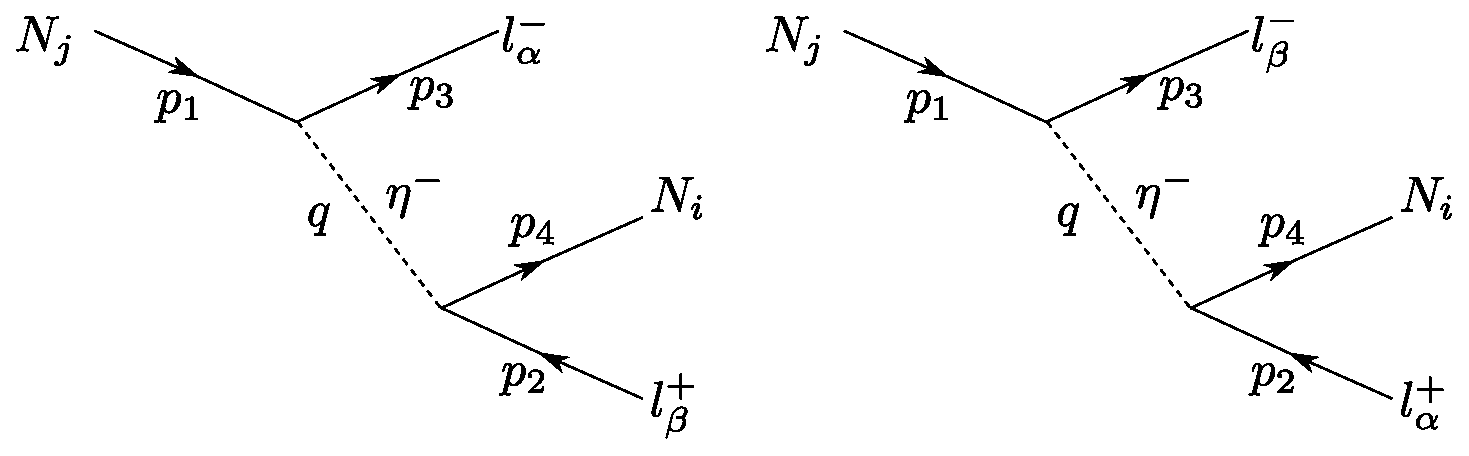
\includegraphics[scale=0.7]{nj_decay} %noinstiki
  \caption{Tree level diagram for $N_j$ decay } %noinstiki
  \label{fig:2} %noinstiki
\end{figure} %noinstiki


we have the amplitude 
\begin{align}
  \mathcal{M}=&-i
  h_{\alpha j}\bar{u}_3(1-\gamma_5)u_1\left(\frac{1}{q^2-M_\eta^2}\right)h_{\beta i}\bar{u}_4(1-\gamma_5)v_2\nonumber\\
  &-i h_{\beta j}\bar{u}_3(1-\gamma_5)u_1\left(\frac{1}{q^2-M_\eta^2}\right)h_{\alpha i}\bar{u}_4(1-\gamma_5)v_2\nonumber\\
  \approx&-\frac{iH_{\alpha\beta ij}}{{M_\eta^2}}\bar{u}_3(1-\gamma_5)u_1\bar{u}_4(1-\gamma_5)v_2
\end{align}
where
\begin{equation}
  H_{\alpha\beta ij}=h_{\alpha j}h_{\beta i}+h_{\alpha i}h_{\beta j}
\end{equation}
\begin{align}
   \mathcal{M}^*=&-\frac{iH_{\alpha\beta ij}}{{M_\eta^2}}
   [\bar{u}_3(1-\gamma_5)u_1]^\dagger[\bar{u}_4(1-\gamma_5)v_2]^\dagger\nonumber\\
   =&-\frac{iH_{\alpha\beta ij}}{{M_\eta^2}}[\bar{u}_1(1+\gamma_5)u_3][\bar{v}_2(1+\gamma_5)u_4]\,.
\end{align}

Multiplying $\mathcal{M}$ and $\mathcal{M}^*$ we have
\begin{align}
\left|\mathcal{M}\right|^2=&\frac{H_{\alpha \beta i j}^2}{M_\eta^4}
[\bar{u}_3^\alpha(1-\gamma_5)_{\alpha\beta}u_1^\beta\bar{u}_1^\gamma(1+\gamma_5)_{\gamma\delta}u_3^\delta]
[\bar{u}_4^\alpha(1-\gamma_5)_{\alpha\beta}v_2^\beta\bar{v}_2^\gamma(1+\gamma_5)_{\gamma\delta}u_4^\delta]\nonumber\\
  =&\frac{H_{\alpha\beta i j}^2}{M_\eta^4}
[u_3^\delta\bar{u}_3^\alpha(1-\gamma_5)_{\alpha\beta}u_1^\beta\bar{u}_1^\gamma(1+\gamma_5)_{\gamma\delta}]
[u_4^\delta\bar{u}_4^\alpha(1-\gamma_5)_{\alpha\beta}v_2^\beta\bar{v}_2^\gamma(1+\gamma_5)_{\gamma\delta}]\nonumber\\
  =&\frac{H_{\alpha\beta i j}^2}{M_\eta^4}
[(u_3\bar{u}_3)_{\delta\alpha}(1-\gamma_5)_{\alpha\beta}(u_1\bar{u}_1)_{\beta\gamma}(1+\gamma_5)_{\gamma\delta}]
[(u_4\bar{u}_4)_{\delta\alpha}(1-\gamma_5)_{\alpha\beta}(v_2\bar{v}_2)_{\beta\gamma}(1+\gamma_5)_{\gamma\delta}]\nonumber\\
=&\frac{H_{\alpha\beta i j}^2}{M_\eta^4}
\operatorname{Tr}[(u_3\bar{u}_3)(1-\gamma_5)(u_1\bar{u}_1)(1+\gamma_5)]
\operatorname{Tr}[(u_4\bar{u}_4)(1-\gamma_5)(v_2\bar{v}_2)(1+\gamma_5)]
\end{align}
Using eq.~\eqref{eq:111}, and neglecting charged fermion masses
\begin{align}
\left|\mathcal{M}\right|^2=&\frac{H_{\alpha\beta i j}^2}{M_\eta^4}
\operatorname{Tr}[\cancel{p}_3(1-\gamma_5)(\cancel{p}_1+M_j)(1+\gamma_5)]
\operatorname{Tr}[(\cancel{p}_4+M_i)(1-\gamma_5)\cancel{p}_2(1+\gamma_5)]\nonumber\\
=&\frac{H_{\alpha\beta i j}^2}{M_\eta^4} L M
\end{align}
\begin{align}
  L=&\operatorname{Tr}[(\cancel{p}_3-\cancel{p}_3\gamma_5)(\cancel{p}_1+\cancel{p}_1\gamma_5+M_j+M_j\gamma_5]
\end{align}
\begin{align}
  L=&\operatorname{Tr}[\cancel{p}_3\cancel{p}_1+\cancel{p}_3\cancel{p}_1\gamma_5+M_j\cancel{p}_3+M_j\cancel{p}_3\gamma_5-\cancel{p}_3\gamma_5\cancel{p}_1-\cancel{p}_3\gamma_5\cancel{p}_1\gamma_5-\cancel{p}_3\gamma_5M_j+M_j\gamma_5]\nonumber\\
  =&2\operatorname{Tr}[\cancel{p}_3\cancel{p}_1]\nonumber\\
  =&2p_3^\alpha p_1^\beta\operatorname{Tr}[\gamma_\alpha\gamma_\beta]\nonumber\\
  =&8p_3^\alpha p_1^\beta g_{\alpha\beta}\nonumber\\
  =&8(p_3\cdot p_1)
\end{align}
Similarly
\begin{align}
  M=8(p_4\cdot p_2)
\end{align}
Therefore
\begin{align}
  \left|\mathcal{M}\right|^2=&\frac{H_{\alpha\beta i j}^2}{M_\eta^4}64(p_3\cdot p_4)(p_1\cdot p_2)\nonumber\\
  \left|\mathcal{M}\right|^2=&\frac{H_{\alpha\beta i j}^2}{4M_\eta^4}4\times64(p_3\cdot p_4)(p_1\cdot p_2)\nonumber\\
\end{align}
In this way, comparing with eq.~\eqref{eq:112}, the results for the moun decay can be directly used after the replacements
\begin{align}
  \frac{g^4}{64 M_W^4}&\to\frac{H_{\alpha\beta i j}^2}{4M_\eta^4}\nonumber\\
  \frac{g^4}{M_W^4}&\to\frac{16H_{\alpha\beta i j}^2}{M_\eta^4}\nonumber\\
  m_\mu&\to M_j\nonumber\\
  x=\frac{m_e}{m_\mu}&\to\frac{M_i}{M_j}\,.
\end{align}
The decay width is according eq.~\eqref{eq:120}
\begin{align}
  \label{eq:121}
  \Gamma(N_j\to l_\alpha^\mp l_\beta^\pm N_i)=&\frac{16H_{\alpha\beta ij}^2}{M_\eta^4}
  \frac{4}{192 (2\pi)^3 M_j }\frac{M_j^6}{16}I\left(x\right)\nonumber\\
=&\frac{(h_{\alpha j}h_{\beta i}+h_{\alpha i}h_{\beta j})^2}{2 M_\eta^4}
  \frac{M_j^5}{192 \pi^3}{}I\left(x\right)
\end{align}
where
\begin{align}
  I(x)=1-8x^2-24x^4\ln(x)+8x^6-x^8\,,\qquad x=\frac{M_i}{M_j}\,.
\end{align}
Similarly the decay through $\eta^0$ is
\begin{align}
  \label{eq:122}
   \Gamma(N_j\to\nu_\alpha\nu_\beta N_i)
=&\frac{(h_{\alpha j}h_{\beta i}+h_{\alpha i}h_{\beta j})^2}{2 M_{\eta^0}^4}
  \frac{M_j^5}{192 \pi^3}{}I\left(x\right)
\end{align}
In this way, for example for $N_2$
\begin{align}
  \sum_{\alpha}\Gamma(N_2\to l_\alpha^- l_\beta^+ N_1)=&\sum_\alpha\frac{h_{\alpha2}^2h_{\beta1}^2+h_{\alpha1}^2h_{\beta2}^2+2h_{\alpha2}h_{\alpha1}h_{\beta2}h_{\beta1}}{2 M_\eta^4}
  \frac{M_2^5}{192 \pi^3}{}I\left(x\right)\nonumber\\
 =&\frac{\mathbf{h}_2^2h^2_{\beta1}+\mathbf{h}_1^2h^2_{\beta2}+2\mathbf{h}_2\cdot\mathbf{h}_1h_{\beta2}h_{\beta1}}{2 M_\eta^4}
  \frac{M_2^5}{192 \pi^3}{}I\left(x\right)
\end{align}
\begin{align}
  \sum_{\alpha\beta}\Gamma(N_2\to l_\alpha^- l_\beta^+ N_1)=&\frac{\mathbf{h}_2^2\mathbf{h}_1^2+\mathbf{h}_1^2\mathbf{h}_2^2
    +2(\mathbf{h}_2\cdot\mathbf{h}_1)^2}{2 M_\eta^4}
  \frac{M_2^5}{192 \pi^3}I\left(x\right)\nonumber\\
=&\frac{\mathbf{h}_1^2\mathbf{h}_2^2
    +(\mathbf{h}_1\cdot\mathbf{h}_2)^2}{M_\eta^4}
  \frac{M_2^5}{192 \pi^3}{}I\left(x\right)
 \end{align}
In general
\begin{align}
  \label{eq:123}
    \sum_{\alpha\beta}\Gamma(N_j\to l_\alpha^- l_\beta^+ N_i)
=&\frac{\mathbf{h}_i^2\mathbf{h}_j^2
    +(\mathbf{h}_i\cdot\mathbf{h}_j)^2}{M_\eta^4}
  \frac{M_j^5}{192 \pi^3}{}I\left(\frac{M_i}{M_j}\right)\nonumber\\
    \sum_{\alpha\beta}\Gamma(N_j\to \nu_\alpha \nu_\beta N_i)
=&\frac{\mathbf{h}_i^2\mathbf{h}_j^2
    +(\mathbf{h}_i\cdot\mathbf{h}_j)^2}{M_{\eta^0}^4}
  \frac{M_j^5}{192 \pi^3}{}I\left(\frac{M_i}{M_j}\right)
\end{align}
For fix $i$ and $j$
\begin{align}
  \label{eq:124}
  \frac{\sum_{\alpha\beta}\operatorname{Br}(N_j\to l_\alpha^- l_\beta^+ N_i)}{\sum_{\alpha\beta}\operatorname{Br}(N_j\to \nu_\alpha \nu_\beta N_i)}=
\frac{M_{\eta^0}^4}{M_{\eta^\pm}^4}
\end{align}
while for 
\begin{align}
  \label{eq:125}
  \frac{\sum_{\alpha\beta}\operatorname{Br}(N_3\to\nu_\alpha\nu_\beta N_2)}{\sum_{\alpha\beta}\operatorname{Br}(N_3\to l_\alpha^-l_\beta^+ N_1)}\approx&
  \frac{\mathbf{h}_2^2\mathbf{h}_3^2
    +(\mathbf{h}_2\cdot\mathbf{h}_3)^2}{\mathbf{h}_1^2\mathbf{h}_3^2
    +(\mathbf{h}_1\cdot\mathbf{h}_3)^2}\frac{M_{\eta^\pm}^4}{M_{\eta^0}^4}I(M_2/M_3)\nonumber\\
  \frac{\sum_{\alpha\beta}\operatorname{Br}(N_3\to l_\alpha^-l_\beta^+ N_2)}{\sum_{\alpha\beta}\operatorname{Br}(N_3\to l_\alpha^-l_\beta^+ N_1)}\approx&
  \frac{\mathbf{h}_2^2\mathbf{h}_3^2
    +(\mathbf{h}_2\cdot\mathbf{h}_3)^2}{\mathbf{h}_1^2\mathbf{h}_3^2
    +(\mathbf{h}_1\cdot\mathbf{h}_3)^2}I(M_2/M_3)
\end{align}

For $N_2$ the total decay width is
\begin{align}
  \Gamma_{\text{tot}}(N_2)=&\left[{\mathbf{h}_1^2\mathbf{h}_2^2
    +(\mathbf{h}_1\cdot\mathbf{h}_2)^2}\right]
  \frac{M_2^5}{192 \pi^3}I\left(\frac{M_1}{M_2}\right)\left[\frac{1}{M_{\eta^\pm}^4}+\frac{1}{M_{\eta^0}^4}\right]
\end{align}
And the individual branchings through $\eta^\pm$ given by eq.~\eqref{eq:121}.

For $N_3$ we have several possibilities for signals with charged leptons. The cleanest one is when $N_3$ decay only through $\eta^\pm$ through an intermediate $N_2$. 

The branching of $N_3$ to two charged leptons plus missing energy is either
\begin{align}
  \label{eq:126}
  \operatorname{Br}(N_3\to l_\alpha^\pm l_\beta^\mp N_1)
\end{align}
where the $N_3$ is reconstructed, or
\begin{align}
  \label{eq:127}
  \operatorname{Br}(N_3\underbrace{\to}_{\eta^0}l_\alpha^\pm l_\beta^\mp N_1)=\operatorname{Br}(N_3\to\nu_\alpha  \nu_\beta N_2)\times\operatorname{Br}(N_2\to l_\alpha^\pm  l_\beta^\mp N_1)
\end{align}
that seem to be very difficult to reconstruct. This also seem to be an irreducible background for
\begin{align}
  \operatorname{Br}(N_2\to l_\alpha^\pm  l_\beta^\mp N_1)
\end{align}
To get rid of processes like the one in eq.~\eqref{eq:127}  must be $\operatorname{Br}(N_3\to\nu_\alpha  \nu_\beta N_2)$ is suppressed. This happens if
\begin{itemize} %noinstiki
\item %noinstiki
 $I(M_2/M3)\ll1$. In this case the mutilepton signal for $N_3$ is also suppressed. Clearly this happens for $M_2\approx M_3$ as $I(x)$ is a sharpest function which controls the kinematical suppression. We show below for an specific point that even for $M_3-M_2\approx20\,$GeV, we can have the Branching in eq.~\eqref{eq:126} sufficiently large.

\item %noinstiki 
$M_{\eta^\pm}\ll M_{\eta^0}$

\end{itemize} %noinstiki


In appendix \ref{sec:sample-point}, it is shown a full set of yukawas consistent with neutrino physics. For this solution 
\begin{align}
  \frac{\operatorname{Br}(\eta^+\to N_3)}{\operatorname{Br}(\eta^+\to N_1)}\approx&0.61&
  \frac{\operatorname{Br}(\eta^+\to N_2)}{\operatorname{Br}(\eta^+\to N_1)}\approx&0.37&\nonumber\\
  {\operatorname{Br}(\eta^+\to N_1)}\approx&0.51&  {\operatorname{Br}(\eta^+\to N_2)}\approx&0.19 & {\operatorname{Br}(\eta^+\to N_3)}\approx&0.30
\end{align}
Below we estimate the branchings to $N_3\to l_\alpha^-l_\beta^+ N_1$ or $N_3\to\nu_\alpha\nu_\beta N_2\to\nu_\alpha\nu_\beta l_\alpha^-l_\beta^+ N_1$. For this we need the Branchings
for $N_2\to l_\alpha^-l_\beta^+ N_1$ compared with Branching to $N_2\to\nu_\alpha\nu_\beta N_1$. In general this is
From this, the visible decays are using eq.~(\ref{eq:124}) 
\begin{align}
   \frac{\sum_{\alpha\beta}\operatorname{Br}(N_2\to l_\alpha^- l_\beta^+ N_1)}{\sum_{\alpha\beta}\operatorname{Br}(N_2\to \nu_\alpha \nu_\beta N_1)}\approx&0.758
   \Rightarrow&\sum_{\alpha\beta} \operatorname{Br}(N_2\to l_\alpha^- l_\beta^+ N_1)=0.431
\end{align}
On the other hand the chanels for $N_3$ are $N_3\to l_\alpha^-l_\beta^+ N_1$, $N_3\to\nu_\alpha\nu_\beta N_1$, $N_3\to l_\alpha^-l_\beta^+ N_2$, and $N_3\to\nu_\alpha\nu_\beta N_2$.
From eqs.~\eqref{eq:124} \eqref{eq:125}
\begin{align}
  \frac{\sum_{\alpha\beta}\operatorname{Br}(N_3\to\nu_\alpha\nu_\beta N_2)}{\sum_{\alpha\beta}\operatorname{Br}(N_3\to l_\alpha^-l_\beta^+ N_1)}
  &\approx0.0812& 
  \frac{\sum_{\alpha\beta}\operatorname{Br}(N_3\to l_\alpha^-l_\beta^+ N_2)}{\sum_{\alpha\beta}\operatorname{Br}(N_3\to l_\alpha^-l_\beta^+ N_1)}
  &\approx0.0615\nonumber\\
\frac{\sum_{\alpha\beta}\operatorname{Br}(N_3\to\nu_\alpha\nu_\beta N_1)}{\sum_{\alpha\beta}\operatorname{Br}(N_3\to l_\alpha^-l_\beta^+ N_1)}
  &\approx1.320
\end{align}
\begin{align}
  \sum_{\alpha\beta}\operatorname{Br}(N_3\to l_\alpha^-l_\beta^+ N_1)&\approx\frac{1}{1+0.0812+0.0615+1.320}=0.406\nonumber\\ 
  \sum_{\alpha\beta}\operatorname{Br}(N_3\to\nu_\alpha\nu_\beta N_1)&\approx0.536\nonumber\\
  \sum_{\alpha\beta}\operatorname{Br}(N_3\to\nu_\alpha\nu_\beta N_2)&\approx0.030\nonumber\\
  \sum_{\alpha\beta}\operatorname{Br}(N_3\to l_\alpha^-l_\beta^+ N_2)&\approx0.025
\end{align}
The expected background for $N_{2,3}\to l_\alpha^-l_\beta^+ N_1$ is 

\begin{equation}
  \sum_{\alpha\beta}\operatorname{Br}(N_3\to\nu_\alpha\nu_\beta N_2)\times\sum_{\alpha\beta}\operatorname{Br}(N_2\to l_\alpha^-l_\beta^+ N_1)\approx0.030\times0.431=0.013
\end{equation}


We have that
\begin{align*}
 \Gamma_{tot}(N_2)=&\left[{\bf h}^2_1{\bf h}^2_2+({\bf h}_1\cdot {\bf h}_2)^2\right]\frac{M_2^5}{192\pi^3}I\left(\frac{M_1}{M_2} \right)\left[ \frac{1}{M^4_{\eta^\pm}}+\frac{1}{M^4_{\eta^0}}\right]\\
\Gamma_{vis}(N_2\to N_1)\equiv& \sum_{\alpha\beta}\Gamma(N_2\to l_\alpha^- l_\beta^+ N_1)\\
   =&\frac{{\bf h}^2_1{\bf h}^2_2+({\bf h}_1\cdot {\bf h}_2)^2}{M^4_{\eta^\pm}}\frac{M_2^5}{192\pi^3}I\left(\frac{M_1}{M_2} \right)\\
\Gamma_{vis}(N_3\to N_1)\equiv& \sum_{\alpha\beta}\Gamma(N_3\to l_\alpha^- l_\beta^+ N_1)\\
   =&\frac{{\bf h}^2_1{\bf h}^2_3+({\bf h}_1\cdot {\bf h}_3)^2}{M^4_{\eta^\pm}}\frac{M_3^5}{192\pi^3}I\left(\frac{M_1}{M_3} \right)\\
\Gamma_{invis}(N_3\to N_2)\equiv& \sum_{\alpha\beta}\Gamma(N_3\to \nu_\alpha \nu_\beta N_2)\\
   =&\frac{{\bf h}^2_2{\bf h}^2_3+({\bf h}_2\cdot {\bf h}_3)^2}{M^4_{\eta^0}}\frac{M_3^5}{192\pi^3}I\left(\frac{M_2}{M_3} \right).
\end{align*}
From above equations we can obtain the following observable:
\begin{align*}
 &\frac{\mbox{Br}_{invis}(N_3\to N_2)\times \mbox{Br}_{vis}(N_2\to N_1)}{\mbox{Br}_{vis}(N_3\to N_1)}\\
&=\frac{\frac{{\bf h}^2_2{\bf h}^2_3+({\bf h}_2\cdot {\bf h}_3)^2}{M^4_{\eta^0}}\frac{M_3^5}{192\pi^3}I\left(\frac{M_2}{M_3} \right)\times \frac{{\bf h}^2_1{\bf h}^2_2+({\bf h}_1\cdot {\bf h}_2)^2}{M^4_{\eta^\pm}}\frac{M_2^5}{192\pi^3}I\left(\frac{M_1}{M_2} \right)}{\frac{{\bf h}^2_1{\bf h}^2_3+({\bf h}_1\cdot {\bf h}_3)^2}{M^4_{\eta^\pm}}\frac{M_3^5}{192\pi^3}I\left(\frac{M_1}{M_3} \right)\Gamma_{tot}(N_2)}\\
&=\frac{{\bf h}^2_2{\bf h}^2_3+({\bf h}_2\cdot {\bf h}_3)^2}{{\bf h}^2_1{\bf h}^2_3+({\bf h}_1\cdot {\bf h}_3)^2}I\left(\frac{M_2}{M_3} \right)\frac{1}{M^4_{\eta^0}\left[\frac{1}{M^4_{\eta^0}}+\frac{1}{M^4_{\eta^\pm}} \right] }\\
&=\frac{{\bf h}^2_2{\bf h}^2_3+({\bf h}_2\cdot {\bf h}_3)^2}{{\bf h}^2_1{\bf h}^2_3+({\bf h}_1\cdot {\bf h}_3)^2}I\left(\frac{M_2}{M_3} \right)\frac{1}{\left[1+\frac{M^4_{\eta^0}}{M^4_{\eta^\pm}} \right]}
\end{align*}
 


% \begin{align}
%   \operatorname{Br}(N_3\to l^\pm l^\mp N_1)=&\sum_{\alpha\beta}\operatorname{Br}(N_3\to l_\alpha^\pm  l_\beta^\mp N_1)+
% \sum_{\alpha\beta}\operatorname{Br}(N_3\to\nu_\alpha  \nu_\beta N_2)\times\sum_{\alpha\beta}\operatorname{Br}(N_2\to l_\alpha^\pm  l_\beta^\mp N_1)\nonumber\\
% \end{align}
% \begin{align}
%   =&\frac{1}{\Gamma_{\text{tor}}(N_3)}\frac{\left[\mathbf{h}_1^2\mathbf{h}_3^2
%     +(\mathbf{h}_1\cdot\mathbf{h}_3)^2\right]}{192\pi^3}
% \end{align}

%\appendix{}
\begin{subappendices} %noinstiki
  

\section{Sample point}
\label{sec:sample-point}

\begin{verbatim} 
       write(32,*) (h(i,1),i=1,3),(h(i,2),i=1,3),(h(i,3),i=1,3)
\end{verbatim} %noinstiki

\begin{verbatim} 
 -0.00188878597  0.000780236776  0.000248251388 
 -0.000352494763 -0.000180683976 -0.00122443053  
  0.000392272581  0.00120920029 -0.0012245638
\end{verbatim} %noinstiki

So that
\begin{align}
  \mathbf{h}_1^2&\approx4.238\times10^{-6}&\mathbf{h}_2^2&\approx1.656\times10^{-6}\nonumber\\
  \mathbf{h}_3^2&\approx3.116\times10^{-6} & \mathbf{h}_1\cdot\mathbf{h}_2&\approx2.208\times10^{-7}\nonumber\\
\mathbf{h}_1\cdot\mathbf{h}_3&\approx1.015\times10^{-7}& \mathbf{h}_2\cdot\mathbf{h}_3\approx&1.143\times10^{-6}
\end{align}
\begin{align}
  \mathbf{h}_1^2\mathbf{h}_2^2+(\mathbf{h}_1\cdot\mathbf{h}_2)^2\approx&7.067\times10^{-12}
  &\mathbf{h}_1^2\mathbf{h}_3^2+(\mathbf{h}_1\cdot\mathbf{h}_3)^2\approx&1.321\times10^{-11}\nonumber\\
  \mathbf{h}_2^2\mathbf{h}_3^2+(\mathbf{h}_2\cdot\mathbf{h}_3)^2\approx&6.465\times10^{-12}
\end{align}
The spectrum consistent with neutrino data is
\begin{align}
  M_1\approx&6.16918656\,\text{KeV} &M_2\approx&22.8695451\,\text{GeV}  &M_3\approx&43.126911\,\text{GeV}\nonumber\\
  M_{\eta^0}\approx&139.1382\,\text{GeV}& M_{\eta^\pm}\approx&149.1382\,\text{GeV}
\end{align}
\begin{align}
  I(M_1/M_3)\approx&1 & I(M_2/M_3)\approx&0.126
\end{align}

\section{Preliminary discussion}
\label{sec:prel-disc}

One interesting possibility in view of the large invisible direct decay, like $N_3\to\nu_\alpha\nu_\beta N_1$, is to get the observables from the missing plus one energetic lepton (coming from $\eta^+$)  signal. May be decays like
\begin{align}
  \eta^+&\to l_\alpha^+ N_3 \to l_\alpha^+ \;\cancel{E}_T\nonumber\\
  \eta^+&\to l_\alpha^+ N_2 \to l_\alpha^+ \;\cancel{E}_T\nonumber\\
\end{align}

Once $\eta^0_{R,I}$, or $\eta^\pm$ are produced the full list of signals is: 
For $\eta^\pm$ production. The decay to $N_j$  is
\begin{align}
\Gamma(\eta^+\to l_\alpha^+ N_j)=\frac{3h_{\alpha j}^2}{16\pi M_\eta}\lambda^{1/2}\left(M_\eta^2,M_j^2,m_\alpha^2\right)\left(1-\frac{M_j^2+m_\alpha^2}{M_\eta^2}\right)
\end{align}
\begin{align}
  \sum_\alpha\Gamma(\eta^+\to l_\alpha^+ N_j)=\frac{3\mathbf{h}_j^2}{16\pi M_\eta}\lambda^{1/2}\left(M_\eta^2,M_j^2,m_\alpha^2\right)\left(1-\frac{M_j^2+m_\alpha^2}{M_\eta^2}\right)
\end{align}
with
\begin{align}
  \lambda^{1/2}\left(M_\eta^2,M_j^2,m_\alpha^2\right)=\left[\left(M_\eta^2+M_j^2-m_\alpha^2\right)^2-4M_\eta^2M_j^2\right]^{1/2}
\end{align}
Neglecting $m_\alpha$ with respect to $N_{2,3}$, we have for $j=2,3$
\begin{align}
  \lambda^{1/2}\left(M_\eta^2,M_j^2,m_\alpha^2\right)\approx&M_\eta^2\left[\left(1+\frac{M_j^2}{M_\eta^2}\right)^2-\frac{4M_j^2}{M_\eta^2}\right]^{1/2}\nonumber\\
  \approx&M_\eta^2\left[1+2\frac{M_j^2}{M_\eta^2}-\frac{4M_j^2}{M_\eta^2}\right]^{1/2}\nonumber\\
  \approx&M_\eta^2\left[1-2\frac{M_j^2}{M_\eta^2}\right]^{1/2}\nonumber\\
  \approx&M_\eta^2\left[1-\frac{M_j^2}{M_\eta^2}\right]
\end{align}
Therefore
\begin{align}
   \sum_\alpha\Gamma(\eta^+\to l_\alpha^+ N_j)\approx&\frac{3\mathbf{h}_j^2M_\eta}{16\pi}\times
   \begin{cases}
     \displaystyle{\left(1-\frac{M_j^2}{M_\eta^2}\right)^2} & j=2,3\\
     1 & j=1
   \end{cases}\nonumber\\
   \approx&\frac{3\mathbf{h}_j^2M_\eta}{16\pi}\times
   \begin{cases}
     \displaystyle{\left(1-2\frac{M_j^2}{M_\eta^2}\right)} & j=2,3\\
     1 & j=1
   \end{cases}\nonumber\\
\end{align}
In this way
\begin{align}
  \Gamma_{\text{tor}}(\eta^+)=&\sum_{\alpha j}\Gamma(\eta^+\to l_\alpha^+ N_j)\nonumber\\
  \approx&\frac{3M_\eta}{16\pi}\left[\mathbf{h}_1^2
    +\mathbf{h}_2^2\left(1-2\frac{M_2^2}{M_\eta^2}\right)
    +\mathbf{h}_3^2\left(1-2\frac{M_3^2}{M_\eta^2}\right)\right]
\end{align}

\begin{align}
\frac{\operatorname{Br}(\eta^+\to N_j)}{\operatorname{Br}(\eta^+\to N_i)}=&  \frac{\sum_\alpha\Gamma(\eta^+\to l_\alpha^+ N_j)}{\sum_\alpha\Gamma(\eta^+\to l_\alpha^+ N_i)}\nonumber\\
\approx&\frac{\mathbf{h}_j^2}{\mathbf{h}_i^2}\frac{1-2M_j^2/M_\eta^2}{1-2M_i^2/M_\eta^2}\nonumber\\
 \approx&\frac{\mathbf{h}_j^2}{\mathbf{h}_i^2}(1-2M_j^2/M_\eta^2)(1-2M_i^2/M_\eta^2)^{-1}\nonumber\\
  \approx&\frac{\mathbf{h}_j^2}{\mathbf{h}_i^2}(1-2M_j^2/M_\eta^2)(1+2M_i^2/M_\eta^2)\nonumber\\
  \approx&\frac{\mathbf{h}_j^2}{\mathbf{h}_i^2}\left[1-2\left(\frac{M_j^2-M_i^2}{M_\eta^2}\right)\right]
\end{align}
For three branchings we should have

\begin{align}
  a+b+c&=1\nonumber\\
1+\frac{b}{a}+\frac{c}{a}&=\frac{1}{a}\nonumber\\
{a}&=\frac{1}{1+{b}/{a}+{c}/{a}}
\end{align}
In this way
\begin{align}
  {\operatorname{Br}(\eta^+\to N_1)}=\frac{1}{1+\frac{\operatorname{Br}(\eta^+\to N_3)}{\operatorname{Br}(\eta^+\to N_1)}+\frac{\operatorname{Br}(\eta^+\to N_3)}{\operatorname{Br}(\eta^+\to N_1)}}
\end{align}

From eq.%~\eqref{eq:75}
\begin{align}
  \frac{\operatorname{Br}\left(N_3\to N_1\right)}
{\operatorname{Br}(N_3\underbrace{\to}_{\eta^\pm}N_2)}=&
\end{align}

\end{subappendices} %noinstiki


%\left(\right)
%\left|\mathcal{M}\right|
%%% Local Variables: 
%%% mode: latex
%%% TeX-master: "beyond"
%%% End:
\begin{thebibliography}{99}
\bibitem{lsm} Diego Restrepo, Hac\'\i a la teor\'\i a cu\'antica de campos, curso web, \url{http://gfif.udea.edu.co}

\bibitem{Maggiore:2005qv}
  M.~Maggiore,
  ``A Modern introduction to quantum field theory,''
%\href{http://www.slac.stanford.edu/spires/find/hep/www?irn=6374123}{SPIRES entry}
{\it  Oxford University Press, 2005. (Oxford Series in Physics, 12. ISBN 0 19 852073 5)}

\bibitem{Mandl:1985bg}
  F.~Mandl and G.~Shaw,
  %``Quantum Field Theory,''
%\href{http://www.slac.stanford.edu/spires/find/hep/www?irn=1457594}{SPIRES entry}
{\it  Chichester, Uk: Wiley ( 1984) 354 P. ( A Wiley-interscience Publication)}

\bibitem{Lahiri:2005sm}
  A.~Lahiri and P.~B.~Pal,
  ``A first book of quantum field theory,''
%\href{http://www.slac.stanford.edu/spires/find/hep/www?irn=6927483}{SPIRES entry}
{\it  Harrow, UK: Alpha Sci. Int. (2005) 380 p}

\bibitem{physics/0703214} Pal, P. ``Representation-independent manipulations with Dirac matrices and spinors'',
	arXiv:physics/0703214v2 [physics.ed-ph]

\bibitem{PD} Wikipedia article: \url{http://en.wikipedia.org/wiki/Particle_decay}

\bibitem{Klasen:2002xi}
  M.~Klasen,
  %``Calculating two- and three-body decays with FeynArts and FormCalc,''
  Int.\ J.\ Mod.\ Phys.\  C {\bf 14} (2003) 1273
  [arXiv:hep-ph/0210426].
  %%CITATION = IMPAE,C14,1273;%%

\bibitem{PeterRenton} \emph{Electroweak Interactions}, Peter Renton


\bibitem{Peskin}
Michael E. Peskin and Daniel V. Schroeder. \emph{An introduction to
Quantum Field Theory}, Addison-Wesley Publishing Company(1995), p.
101

\bibitem{Peskin1}
ibdg 1, p. 105

\bibitem{Halzen}
Francis Halzen and Alan D. Martin. \emph{Quarks} \& \emph{Leptons:
An introductory Course in Modern Particle Physics}, John Wiley \&
Sons(1984), p. 89

\bibitem{Quigg}
Chris Quigg. \emph{Gauge theory of the Strong, Weak and
Electromagnetic Interactions}, Westview Press(1997), p. 110


\bibitem{Quigg1}
ibdg 4, p. 130.

\bibitem{Mandl1}
ibdg 5, p. 325.


\bibitem{Sierra:2008wj}
  D.~Aristizabal Sierra, J.~Kubo, D.~Restrepo, D.~Suematsu and O.~Zapata,
  ``Radiative seesaw: Warm dark matter, collider and lepton flavour violating
  signals,''
  Phys.\ Rev.\  D {\bf 79} (2009) 013011
  [arXiv:0808.3340 [hep-ph]].
  %%CITATION = PHRVA,D79,013011;%%

\bibitem{Gross:1993} 
Relativistic Quantum Mechanics and Field Theory, Franz Gross, John Wiley \& Sons, INC. 1993

\bibitem{McMahon:2009zz}
  D.~McMahon,
  ``Quantum field theory demystified: A self-teaching guide,''
  \href{http://www.slac.stanford.edu/spires/find/hep/www?irn=8432112}{SPIRES entry}
{\it  New York, USA: McGraw-Hill (2009) 299 p}

\bibitem{Feynman:1986er}
  R.~P.~Feynman,
  ``QED. The Strange Theory Of Light And Matter,''
%\href{http://www.slac.stanford.edu/spires/find/hep/www?irn=1631209}{SPIRES entry}
{\it  Princeton, Usa: Univ. Pr. ( 1985) 158 P. ( Alix G. Mautner Memorial Lectures)}


\bibitem{Semenov:2008jy}
  A.~Semenov,
  ``LanHEP - a package for the automatic generation of Feynman rules in field
  theory. Version 3.0,''
  Comput.\ Phys.\ Commun.\  {\bf 180} (2009) 431
  [arXiv:0805.0555 [hep-ph]], \url{http://feynrules.phys.ucl.ac.be/}.
  %%CITATION = CPHCB,180,431;%%

\bibitem{Christensen:2008py}
  N.~D.~Christensen and C.~Duhr,
  ``FeynRules - Feynman rules made easy,''
  Comput.\ Phys.\ Commun.\  {\bf 180}, 1614 (2009)
  [arXiv:0806.4194 [hep-ph]],
   \url{http://feynrules.phys.ucl.ac.be/}.
  %%CITATION = CPHCB,180,1614;%%

\bibitem{massivephoton}
  Christianto V., Smarandache F., and Lichtenberg F., 
  ``\href{http://www.ptep-online.com/index_files/2009/PP-16-08.PDF}{A Note of Extended Proca Equations and Superconductivity,}''
  Progress in Physics, \textbf{1} (2009) 40
  [viXra:1003.0054]

\end{thebibliography}
%%% Local Variables: 
%%% mode: latex
%%% TeX-master: "beyond"
%%% End:

\end{document}


%%% Local Variables: 
%%% mode: latex
%%% TeX-master: "beyond"
%%% End: 
